\documentclass[openany,12pt]{book}

% Encoding and Language
\usepackage[utf8]{inputenc}
\usepackage[english]{babel}

% Mathematics Packages
\usepackage{amsmath, amssymb, amsfonts, amsthm, mathtools, mathabx}

% Geometry and Formatting
\usepackage[a4paper,left=30mm,right=20mm,top=30mm,bottom=25mm]{geometry}
\usepackage{float}
\usepackage{enumitem}
\usepackage{varioref}
\usepackage{nicefrac}

% Colors and Graphics
\usepackage{xcolor, graphicx}

% Tables and Lists
\usepackage{multirow, booktabs}
\usepackage{siunitx}
\usepackage{caption, subcaption}

% TikZ and PGFPlots
\usepackage{tikz}
\usepackage{pgfplots}
\pgfplotsset{compat=1.18}
\usepgfplotslibrary{external} 
\tikzexternalize
\tikzset{external/mode=graphics if exists}
\usetikzlibrary{external}

% Algorithms
\usepackage{algorithm, algpseudocode}

% Other Useful Packages
\usepackage{comment, pdflscape, diagbox}
\usepackage[colorinlistoftodos]{todonotes}

% Bibliography
\usepackage{biblatex}
\addbibresource{biblio.bib}

% Custom Commands
\newcommand{\norm}[1]{\lVert #1 \rVert}
\newcommand{\hcu}[1]{H_{0}^{1}(#1)}
\newcommand{\R}{\mathbb{R}}
\newcommand{\N}{\mathbb{N}}
\newcommand{\om}{\Omega}
\newcommand{\ga}{\Gamma}
\newcommand{\ind}{\mathbf{I}}
\newcommand{\sign}{\mathrm{sign}}
\newcommand{\fsparse}{\Upsilon}
\newcommand{\reals}{\mathbb{R}}
\newcommand{\extreals}{\overline{\mathbb{R}}}
\newcommand{\warrow}{\rightharpoonup}
\renewcommand{\l}{\left}
\renewcommand{\r}{\right}
\renewcommand{\div}{\text{div\,}}
\newcommand{\arrow}{\rightarrow}

% Mathematical Operators
\DeclareMathOperator{\argmin}{argmin}
\DeclareMathOperator{\meas}{meas}
\DeclareMathOperator{\jump}{\jmath}
\DeclareMathOperator*{\esssup}{ess\;sup}
\DeclareMathOperator{\dom}{dom}
\DeclareMathOperator{\epig}{epig}

% Theorem Environments
\newtheorem{assumption}{Assumption}[chapter]
\newtheorem{proposition}[assumption]{Proposition}
\newtheorem{definition}[assumption]{Definition}
\newtheorem{lemma}[assumption]{Lemma}
\newtheorem{remark}[assumption]{Remark}
\newtheorem{corollary}[assumption]{Corollary}
\newtheorem{theorem}[assumption]{Theorem}
\newtheorem{example}{Example}

% Number equations within sections
\numberwithin{equation}{chapter}

% Paragraph Formatting
\setlength{\parindent}{0cm}

\begin{document}

%\pagestyle{empty}
\begin{center}	\bf
	\LARGE { ESCUELA POLITÉCNICA NACIONAL}\vspace{8mm}
\end{center}


\begin{center}	\bf
	\Large {DEPARTAMENTO DE MATEMÁTICA}\vspace{3mm}
\end{center}

\begin{center}	\bf
	\Large {DOCTORADO EN MATEMÁTICA APLICADA}\vspace{15mm}
\end{center}

\begin{center}	\bf
	\Large {OPTIMAL CONTROL OF NON CONVEX SPARSITY PROBLEMS GOVERNED BY ELLIPTIC PARTIAL DIFFERENTIAL EQUATIONS}
	\vspace{20mm}
	
	\large{TESIS PREVIA A LA OBTENCIÓN DEL TÍTULO DE DOCTOR EN MATEMÁTICA APLICADA}\vspace{15mm}
	

	
	\normalsize{DIEGO MAURICIO VARGAS JARAMILLO}\\
	diego.vargas@epn.edu.ec\vspace{13mm}
	
	\normalsize{DIRECTOR: DR. PEDRO MARTÍN MERINO ROSERO}\\
	pedro.merino@epn.edu.ec\vspace{6mm}
	
	\vspace{15mm}
	
	\normalsize{QUITO, }
\end{center}
%\pagestyle{empty}
\vspace*{30mm}
\begin{center}
	DECLARACIÓN
\end{center}

Yo, Diego Mauricio Vargas Jaramillo, declaro bajo juramento que el trabajo aquí descrito es de mi autoría; que no ha sido previamente presentada para ningún grado o calificación profesional; y, que he consultado las referencias bibliográficas que se incluyen en este documento.\\

La Escuela Politécnica Nacional puede hacer uso de los derechos correspondientes a este trabajo, según lo establecido por la Ley de Propiedad Intelectual, por su Reglamento y por la normatividad institucional vigente.\vspace{30mm}

\begin{center}
	
	Diego Mauricio Vargas Jaramillo
\end{center}
%\pagestyle{empty}
\vspace*{30mm}
\begin{center}
CERTIFICACIÓN
\end{center}
\vspace{20mm}
Certifico que el presente trabajo fue desarrollado por \textbf{Diego Mauricio Vargas Jaramillo}, bajo mi supervisión.\vspace{40mm}


\begin{center}
	
	Dr. Pedro Martín Merino Rosero\\
	DIRECTOR
	
	

\end{center}
%\include{agradecimiento}
%\tableofcontents
%\include{intro}
%\chapter*{Introduction}
\addcontentsline{toc}{chapter}{Introduction}

Optimal control problems with nonconvex cost functions are widely used in a great number of practical and theorical problems, such as inverse problems in biomedical or seismic imaging, certain energy efficiency models (see \cite{vogel}), image restoration (see \cite{hintermueller}), compressed sensing (see \cite{foucart}), optimal control problems (see \cite{casas}), and other applications. Their importance relies on the properties that the nonconvexity can provide to the optimal control solution, such as the sparsity. Of course, this desirable feature over the control is not only induced exclusively by nonconvex cost functions; for example, Georg Stadler \cite{stadler2006} proposed a control problem with a $L^1$ penalizer governned by a elliptic partial differential equation and control pointwise constrains, and showed that the optimal control solution is sparse over a subset of its domain. Therefore, we see that it is possible to induce sparsity over the optimal control of a problem choosing a suitable penalization. However, the cost functional used in \cite{stadler2006} is convex but not differentiable.\\

Thus, the natural question which arises from the sparsity of the control is that if we can `maximise' as much as possible the subset of its domain where the sparsity appears. One possibility to address this is the use a $L^0$ penalizer in the cost function \cite{ito-kunisch2014}, because this one is linked to the minimization of the measure of the support of the control. However, this penalization is not even a norm-type penalization, and lack of convexity and differentiability is evident. Hence, in order to induce sparsity of the optimal control we can use this kind of penalizations at cost of the loss of convexity of the cost function. In fact, the work of Kasumufi Ito and Karl Kunisch \cite{ito-kunisch2014} show us that, if we use a $L^q$ penalizer, with $q\in [0,1)$, sparsity of the control is assured. Unfortunately, the loss of convexity is inherent to this type of problems, causing that the standard tools of the Convex Analysis and Functional Analysis can not be used for proving aspects such as existence and unicity of solutions for the problem and its regularity, or deducing optimally systems and subsequently the numerical treatment of this problems. \\

Between the $L^1$ and $L^0$ penalizers, it can be considerated $L^q$ penalizers with $q\in [0,1)$, which, in some sense, can be considered as natural aproximations of the $L^0$ penalizer \cite{merino2019} as $q\to 0$. However, there are notable features of the sparsity induced in the optimal control which arise from this particular kind of penalized problems, specially that the jump discontinuities of the optimal control can be characterized by a constant with depends on the problem parameters and appears at its boundary's support. This property can be used in practical problems which needs a sharp localized action of the control within the domain. Despite this, the lack of convexity in the cost function is inevitable, which makes  its theoretical and numerical treatment challenging as we pointed out before.\\

In order to study the sparsity induced by the $L^q$ penalizer, a regularization or a relaxation of this term can be used, see for example \cite{ekeland}, \cite{shane}, \cite{warga}. However, it could happen that the these properties become weaker than the non regularized problem. Instead of this, Ito and Kunisch in \cite{ito-kunisch2014} propose a Pontryagin-type principle with allow us to characterise the jumps of the control under certain hypothesis of the functions involved in the control problem. One advantage of this approach is that, if a control problem satisfies the hypothesis proposed in \cite{ito-kunisch2014}, and has an optimal control, then its sparsity can be studied through a uni dimensional problem. However, the imposition of the existence of a solution for the control problem is required, being the real existence of it as an assumption. In fact, the optimal control problem treated in \cite{ito-kunisch2014} involves an $H_{0}^{1}$ norm of the control, which allow them to prove existence of an optimal solution under compacity arguments. Pedro Merino in \cite{merino2019} study a similar problem than Ito and Kunisch, but changing the $H_0^1$ norm with a classical $L^2$ Tikhonov term. Nevertheless, a Huber-type regularization is proposed in order to carry out with the nonconvex $L^q$ term, making that the sparse properties of the control dependents on the Huber regularization term. Despite this, he proved that the regularized control problem has an optimal solution, and moreover, a optimally system can be deduced with enough regularity to propose a numerical scheme to solve it, using the so called DC-Algorithm. A latter work of the same author propose a Semi Smooth Newton method for solving the problem.\\

The question of the existence of an optimal solution for this kind of problems, without using regularization or the non convex term such as additional terms in the cost function that allow the use of compacity arguments was thereby open. This problem motivate us to investigate a way to obtain the existence of an optimal control solution for this kind of problems, and later to characterise its sparsity properties. The use of the tools proposed by Ito and Kunisch are useful for our work, and allow us to extend them for deriving an optimally system that allow us to construct a solution for the $L^q$ problem, without regularizing or relaxing it.\\

On the other hand, it can be proposed a relaxation of the cost function of the problem which involves both the Tikhonov term and the nonconvex penalty $L^q$, using the so called  \textit{Convex Regularization} of the uni dimensional version of this terms. Specifically, we discover that the convexified problem allow us to construct an optimal solution for the original problem, without the requirement of the regularization of the non convex term using additional parameters such as in the Huber regularization case, and only through its optimally system. Moreover, we find that the optimally system of the convexified problem is nearly equivalent than the first approach we present, but each one constructed by different theoretical approaches. In addition, the convexified problem provide us tools to deduce a priori error estimates for solving numerically the original problem using a finite elements approach.\\

The optimal control problems discussed so far may have point-wise control restrictions. In fact, the Pontryagin-type principle used in our investigation is derived for a control problems with this kind of restrictions; however, if we impose point-wise state constraints instead of control ones in the non convex penalized problems, we deal with additional difficulties in order to prove the existence of solutions, such as the derivation of an optimally system that allow us to study numerically the problem. Optimal control problems with point-wise state constrains but convex cost functions are widely studied, we refer to \cite{casas, casas-clason-kunisch2012, casas-delosreyes}. The main difficult present in this kind of problems is that their optimally systems present Lagrange multipliers with low regularity, such as Borel regular measures. In order to deal with this issue, Christian Meyer et al. proposed in \cite{meyer-2007} a Lavrentiev-type regularization with mix state and control in a new artificial control variable, which depends on a regularization parameter. This change of variable allow them to derive a more regular optimally system which is used to derive a numerical method for solving the problem. However, the convexity of the cost function is crucial for studying the limit of the family of problems linked to the regularization parameter.\\

In our particular case, the lack of convexity difficult the theoretical treatment of the problem with point-wise state constrains. However, the convex relaxation, plus a combination of mixed control-state point-wise constrains in the problem allow us to study the pure state constrained one. \\

Respect to the numerical treatment of our problem, we present three different schemes: the Sequential Quadratic Hamiltonian Algorithm, the Difference of Convex functions Algorithm, and the Semismooth Newton Algorithm. The first scheme can be applied directly to the control constrained problem without a regularization or a explicit computation of its optimally system. However, in order to ensure its convergence, a sufficient descent condition which depends on the Hamiltonian of the problem must be imposed, and therefore, this method could be restrictive for a general optimal control problems. In addition, since this method needs to solve a point-wise one dimensional minimization problem at each node of the discretized domain, an additional computational power could be needed. The first issue about this method can be carried out by the favorable structure of the Hamiltonian of our problem, while the second one can be solved with parallelization of the computations.\\

The second method, Difference of Convex algorithm, was first introduced in a finite dimensional optimization frame. Several works about this method are \cite{dinh, dihn2, dihn3, dinh4}, and many other papers. In contrast, the application of this method in infinite dimensional context is novel, and works such as of Yongdo Lim et. al \cite{yongdo} present extensions to the DC algortihm for optimizaction in Hilber spaces. In the particular case of control problems with $L^q$ penalizers, \cite{merino2019} presents a numerical scheme  to the regularized control problem based on the DC algorithm. The main advantage behind this method is that, since the cost function can be split into the difference of two convex functions, and one of them has a closed subdifferential, it is easy to construct part of the algorithm explicit. Despite this, to end a complete iteration of the algorithm, a $L^1$ control constrained problem must be solved.\\

The third method, Semi smooth Newton algorithm, was proposed for solving system of equations which have certain regularity (semismoothness regularity). The finite dimensional form of this algorithm was introduced by Mifflin in \cite{mifflin}, and its extension for infinite dimensional spaces was introduced by several wors, included \cite{qi, qisun}. For the $L^q$ penalized control constrained problem, \cite{merino2021} proposed an hybrid method which combines the Semismooth Newton method and the DC method. However, this method is specially useful for the numerical treatment of the $L^q$ penalized method with point-wise state constrains, but applied first with a regularization first over the constrains, following a Lavrentiev type regularization, proposed by \cite{meyer-2007}.\\

Our contributions in this work are the following:

\begin{itemize}
    \item We prove the existence of a generalized control solution to a $L^q$ penalized problem with control point-wise constrains, defining a thresholding operator which extends the methodology proposed by \cite{ito-kunisch2014}.
    \item  We prove the existence of a solution for the penalized $L^q$ control problem, with mixed control-state point-wise constrains, such as a pure point-wise state constrain problem.
    \item We establish the best numerical algorithm for solving the penalized problem with control point-wise constrains, facing up three different numerical algorithms, through a extensively set of numerical experiments.
    \item We address a model...
\end{itemize}

This work is organized as follows: the first chapter is devoted to a review of some theoretical results about Functional Analysis and Convex Analysis that will be useful through the thesis. 


\chapter{Preliminars}
\section{Functional Spaces}

Trough this Chapter, $\om\subset \mathbb{R}^n$, $n=2,3$ represents an open boundary with Lipschitz-type boundary $\Gamma$. In addition, for a general Hilbert space $X$, and for some $C\subset X$, we denote as $\mathbf{I}_{C}:X\to \{0,+\infty\}$ the indicator function over $C$, which takes the value $\mathbf{I}_{C}(x)=0$ if $x\in C$, and $I_{C}(x)=+\infty$ if $x\notin C$. Well known properties of $\mathbf{I}_{C}$ tell us that this function is lower semicontinuous only if $C$ is closed, and convex only if $C$ is convex, see for example \cite{combettes} for a detailed discussion of these results. 

As usual, in a Hilbert space $X$, we denote as $(\cdot,\cdot)_{X}$ its inner product, and, for a general setting, if $X$ is a general Banach space, and $f\in X^*$, the action of $f$ over any $x\in X$ is denoted as $\langle f,x\rangle_{X^{*},X}$. In addition, if we define as $\mathcal{L}(X,Y)$ the space of linear bounded mappings from two Banach spaces $X, Y$, the norm of any $L\in \mathcal{L}(X,Y)$ is defined as usual:
\[
\norm{L}_{\mathcal{L}(X,Y)}=\sup_{\norm{x}_{X}=1}=\norm{Lx}_{Y}.
\]
Finally we recall the Riesz representation Theorem: if $X$ is a Hilbert space, then for ay $f\in X^*$ there exists a unique $u_f\in X$ such that
\[
\langle f, x\rangle_{X^{*},X}=(u_{f},x), \quad \mbox{for all }x\in X.
\]
Therefore, in the context of Hilbert spaces, we use the notation $(\cdot,\cdot)_{X}$ for both inner product and action of the elements of the dual space of $X$ over $X$.

The set of real-valued Lebesgue measurable functions with domain $\om$ is denoted as $M(\om)$.  We recall the definition of Caratheodory functions and Nemitski operators, taken from \cite{ambrosetti}.

\begin{definition}[Caratheodory function]
    Let $f:\om\times \mathbb{R}\to \mathbb{R}$ a function. We say that $f$ is Caratheodory if 
    \begin{enumerate}
        \item $s\mapsto f(x,s)$ is continuous for almost all $x\in \om$,
        \item $x\mapsto f(x,s)$ is measurble for all $s\in\mathbb{R}$.
    \end{enumerate}
\end{definition}


\begin{definition}[Nemitski operator]
    Let $f:\om\times \mathbb{R}\to \mathbb{R}$ a Caratheodory function. The Nemitski operator associated to $f$ is the map $N: M(\om)\to \mathbb{R}$ defined as:
    \[
    N(u(x))=f(x,u(x)).
    \]
\end{definition}
To avoid introducing additional notation, we use the same symbol $f$ to denote its associated Nemitski operator.

We recall a well-known result about continuity of Nemitski operators, see \cite{ambrosetti} for a detailed proof of this fact.

\begin{theorem}
    Let $f:\om\times\mathbb{R}\to \mathbb{R}$ a Caratheodory function such that, for  $p, q\ge 1$ and some constants $a, b>0$,
    \[
    |f(x,s)|\le a + b|s|^{\frac{p}{q}}.
    \]
    Then, the Nemitski operator $f$ is continuous from $L^p(\om)$ to $L^q(\om)$.
\end{theorem}
The standar notation $L^p(\om)$ is used for the set Lebesgue $p-$integrable functions, see \eqref{def:l^p_space}.  

Let $k\in \mathbb{N}_*$. A \textit{multi-index of order k} is a vector $\alpha=(\alpha_1,\cdots,\alpha_k)^{\top}\in \mathbb{N}^k$. The \textit{order} of $\alpha$ is defined as
\[
|\alpha|=\sum_{i=1}^k \alpha_i
\]
Let $\om\subset\reals^n$ an open set, and $f:U\to \reals$. The notation $D^\alpha f(x)$ for $x\in U$ stands for
\begin{equation}\label{def:weak_derivate}
D^\alpha f(x):=\frac{\partial^{|\alpha|}f(x)}{\partial x_1^{\alpha_1}\cdots\partial x_n^{\alpha_k}},
\end{equation}
whenever the partial derivative of the right hand exists. $f:\om\to\reals$ is said to be of class $C^k(\om)$ if $D^{\alpha}f(x)$ exists and is continuous for any $\alpha\in\mathbb{N}^k$ such that $|\alpha|\le k$. We denote as $C^{k}(\bar \om)$ the set of functions $f:\om\to \reals$ in $C^{k}(\om)$ which derivatives $D^{\alpha} f(x)$ are uniformly continuous for all $\alpha\in\mathbb{N}^k$ such that $|\alpha|\le k$. The \textit{support} of a function $f:\om\to \reals$ is the set $$\mbox{supp }f:=\{x\in \om: f(x)\ne 0\};$$the set $C_0(\om)$ represents respectively the sets of continuous functions over $\om$ with compact support, and $C^k_0(\om)$ the set of functions in $C^k(\om)$ at which the function as their derivatives have compact support. The same holds for the set $C^{\infty}_0(\om)$\\

Let $p\in [1,\infty[$. The functional space $L^p(\om)$ is defined as
\begin{equation}\label{def:l^p_space}
L^p(\om):=\l\{f:\om\to \reals: f \mbox{ is measurable}, \int_{\om}|f(x)|^p\; dx<\infty\r\}.
\end{equation}
Recall that a property holds \textit{almost everywhere} in a set $\om\subset \reals^n$, also said that the property holds \textit{almost all} $x\in \om$ if there exists a set $A\subset\om$  with measure equal to zero at which the property does not hold. The space $L^{\infty}(\om)$ is defined as the space of measurable functions $f:\om\to \reals$ such that there exists a positive constant $C$ such that
\[
|f(x)|\le C,\quad \mbox{almost all }x\in \om.
\]
The $L^p(\om)$ spaces are Banach spaces with the norm
\[
\norm{f}_{L^p(\om)}=\l(\int_{\om}|f(x)|^p\r)^\frac{1}{p},
\]
for $1\le p<\infty$, and 
\begin{equation}\label{def:essup}
    \norm{f}_{L^{\infty}(\om)}:=\sup\{C>0: |f(x)|\le C\mbox{ almost all }x\in \om \}.
\end{equation}

The right hand side of \eqref{def:essup} is also called the essential supremum of $f$, and is denoted as $\esssup_{x\in \om}|f(x)|$.

Recall that $L^p(\om)$ is reflexive and separable for $p\in ]1,\infty[$. Due to the Riesz representation Theorem, we have in addition that $\l(L^p(\om)\r)^*=L^q(\om)$ for $q\in ]1,\infty[$ such that $\frac{1}{p}+\frac{1}{q}=1$. In addition, $\l(L^1(\om)\r)^*=L^\infty(\om)$. and $\l(L^\infty(\om)\r)^*\subsetneq L^1(\om)$.\\

Let $p,q \in [1,\infty]$ such that $\frac{1}{p}+\frac{1}{q}=1$ (we assume that if $p=1$, $q=\infty$ and vice versa). Then, if $f\in L^p(\om)$ and $g\in L^q(\om)$, we recall the \textit{Hölder inequality Theorem:} $fg\in L^{1}(\om)$ and
\[
\int_{\om}|f(x)g(x)|\; dx\le \norm{f}_{L^p(\om)}\norm{g}_{L^q(\om)}.
\]

For a complete proof of Hölder inequality, see for example \cite{brezis2010}. Recall that a function $f:\om\to\reals$ is the class of $L^1_{\mbox{loc}}(\om)$ if the integral
\[
\int_{K}|f(x)|\; dx<\infty,
\]
for every compact set $K\subset \om$.  Let $f,g\in L^1_{\mbox{loc}}(\om)$ and $\alpha\in \mathbb{N}^k$ a multiindex. The function $g$ is called the $k-$th \textit{weak derivative} of $f$, noted as $D^\alpha f=g$, if
\[
\int_{\om}f D^{\alpha}\varphi \; dx=(-1)^{|\alpha|}\int_{\om}g \varphi \; dx,
\]
for any $\varphi\in C^{\infty}_0(\om)$. We point out that the notation \eqref{def:weak_derivate} is also used for the weak derivatives of $f$. 
Let $p\in [1,\infty]$ and $k\in \mathbb{N}$, the \textit{Sobolev space} $W^{k,p}(\om)$ is the space of functions defined as
\[
W^{k,p}(\om):=\{f\in L^p(\om): D^{\alpha}f\in L^p(\om) \mbox{for all }\alpha\in \mathbb{N}^{k}, |\alpha|\le k\}.
\]
The space $W^{k,p}_0(\om)$ is the closure of $C^{\infty}_0(\om)$ into $W^{k,p}(\om)$. As usual, the space $W^{1,2}(\om)$ is represented by $H^1(\om)$, and the same holds for $W^{1,2}_0(\om)=H_0^1(\om)$.\\

The next result shows us important embeddings for the studying of the regularity of the solution for a P.D.E.

\begin{theorem}[Rellich-Kondrachov embedding Theorem] Let $\om\subset \reals^n$ a bounded Lipschitz domain. Let $p\in ]1,\infty[$ and $k\in \mathbb{N}_{*}$. Then, the following embeddings exist and are continuous:
\begin{enumerate}
    \item for $kp<n$: $W^{k,p}(\om)\hookrightarrow L^q(\om)$, if $1\le q\le \frac{np}{n-kp}$,
    \item for $kp=n$, $W^{k,p}(\om)\hookrightarrow L^q(\om)$, if $1\le q<\infty$,
    \item for $kp>n$, $W^{k,p}(\om)\hookrightarrow C(\bar \om)$
\end{enumerate}
    
\end{theorem}

\section{Linear Partial Differential Equations of second order}
Through this work, we mainly focus on the following kind of Partial Differential Equations: given measurable functions $a_{ij}, b_{i}$ and $c$, for $i,j\in \{1,\cdots, n\}$ with $a_{ij}\not\equiv 0$ for some $i,j$, we denote the \textit{second order partial differential operator} $A$ as
\begin{equation}\label{eq:operator_A}
    (Ay)(x)=-\sum_{i,j=1}^{n}\frac{\partial y(x)}{\partial x_i}\l(a_{ij}(x) \r)+\sum_{i=1}b_{i}(x)\frac{\partial y(x)}{\partial x_i}+c(x)y(x).
\end{equation}

Then, for a given function $u$, the problem:
\begin{equation}\label{eq:elliptic_pde}
\begin{cases}
    Ay=u, &\mbox{in }\om,\\
    y=0, &\mbox{on }\Gamma,
\end{cases}
\end{equation}
is called a second order partial differential equation. In our setting. Now, we say that the operator $A$ is uniformly elliptic if there exists a constant $\theta>0$ such that
\[
\sum_{i,j =1}^n a_{ij}(x)\xi_i\xi_j\ge \theta \norm{\xi}_2^2,
\]
for almost all $x\in \om$ and any $\xi \in\mathbb{R}^n$. The notation $\norm{\cdot}_2$ stands for the Euclidean norm in $\mathbb{R}^n$. 

For any $y,z \in H_0^1(\om)$, we define 
\begin{equation}\label{eq:bilinear_form}    a(y,z):=\int_{\om}\l(\sum_{i,j=1}^{n} a_{ij}(x)\frac{\partial y(x)}{\partial x_i}\frac{\partial z(x)}{\partial x_{j}}\; dx+\sum_{i=1}^{n}b_i(x)\frac{\partial y(x)}{\partial x_i}z(x)+c(x)y(x)z(x) \r)\; dx.
\end{equation}

$a$ is called the \textit{bilinear form associated to $A$}. Remember that a function $y\in H_0^1(\om)$ is called a solution to \eqref{eq:elliptic_pde} if

\begin{equation}\label{eq:variational_formulation}
a(y,z)=(u,z)_{L^2(\om)}, \quad \mbox{for all }z\in H_0^1(\om)
\end{equation}

The relation \eqref{eq:variational_formulation} is also called the \textit{variational formulation} of \eqref{eq:elliptic_pde}.

Assuming that $A$ is coercive, $a_{ij}\in L^{\infty}(\om)$ and $c(x)\ge 0$ almost all $x\in\om$ it can be shown that the equation \eqref{eq:elliptic_pde} has a unique solution for any $u\in L^2(\om)$, see \cite[Remark 23]{brezis}. However, for results about regularity of solutions, it is necessary to introduce the concept of Lipschitz type domains.
 
 \begin{definition}
Let $\Omega \subset \mathbb{R}^n$, $n \ge 2$, be a bounded domain with boundary $\Gamma$.
We say that $\Omega$, or $\Gamma$, belongs to the class $C^{k,1}$, $k \in \mathbb{N}\cup\{0\}$,
if there exist finitely many local coordinate systems $S_1,\dots,S_M$,
functions $h_1,\dots,h_M$, and numbers $a>0$ and $b>0$ such that the following
properties hold:
\begin{enumerate}[label=(\roman*)]
\item
The functions $h_i$, $1 \le i \le M$, are $k$-times differentiable on the closed
$(N-1)$-dimensional cube
\[
\overline{Q}_{N-1}
= \left\{ y=(y_1,\dots,y_{N-1}) : |y_i| \le a,\ i=1,\dots,N-1 \right\},
\]
and the partial derivatives of order $k$ are Lipschitz continuous on
$\overline{Q}_{N-1}$.

\item
For any $P \in \Gamma$ there exists some $i \in \{1,\dots,M\}$ such that in the
coordinate system $S_i$ there is some $y \in Q_{N-1}$ with
\[
P = (y, h_i(y)).
\]

\item
In the local coordinate system $S_i$ we have
\[
(y,y_N) \in \Omega
\iff
y \in \overline{Q}_{N-1}, \quad h_i(y) < y_N < h_i(y)+b,
\]
\[
(y,y_N) \notin \Omega
\iff
y \in \overline{Q}_{N-1}, \quad h_i(y)-b < y_N < h_i(y).
\]
\end{enumerate}
\end{definition}

 \begin{definition}
     A domain $\om$ with boundary of class $C^{0,1}$ are called Lipschitz-type domain.
 \end{definition} 
 
 Now, if $b_i\equiv 0$ for all $i\in \{1,\cdots,n\}$, the following result follows:

 \begin{theorem}
     Suppose that $\om$ is a Lipchitz-type domain, $a_{ij}\in L^{\infty}(\om)$, $b_i\equiv 0$ and $c(x)\ge 0$ for almost all $x\in \om$. Then, \eqref{eq:elliptic_pde} has a unique solution $y\in H_0^1(\om)$ for every $u\in L^2(\om)$. Moreover, we have that there exists a constant $\nu>0$ such that 
     \[     \norm{y}_{H_0^1(\om)}\le \nu \norm{u}_{L^2(\om)}.
     \]
 \end{theorem}
For a proof of this Theorem, we refer to \cite[Theorem 2.7]{troeltzsch2010}.

\subsection{Regularity of solutions}

Up to this point, we have established conditions that guarantee the existence and uniqueness of solutions to the equation \eqref{eq:elliptic_pde}. However, in order to derive error estimates within the framework of the finite element method (FEM), it is essential to investigate the regularity of weak solutions. Indeed, several results that will be used throughout this work rely on the fact that weak solutions possess a higher degree of regularity than $H_0^1$.

One possible strategy to improve the regularity of solutions consists in imposing stronger smoothness assumptions on the domain, for instance by considering domains of class $C^2$, as will be discussed later. Another way to enhance the regularity is to require the coefficients $a_{ij}$ to satisfy stronger regularity assumptions than merely belonging to $L^{\infty}$. Nevertheless, such assumptions may exclude a large class of admissible domains or coefficient configurations in which optimal control problems can naturally be posed.

For this reason, we will subsequently present regularity results that can be achieved for polygonal domains and coefficients with limited smoothness. These results are sufficient for the purposes of this work and do not require a highly regular boundary nor overly restrictive assumptions on the coefficients. 

The following Theorems are an example of the discussion above. First of all, the following Theorems require more regularity of the coefficients. Their demonstrations can be found in \cite{evanspde}.

\begin{theorem}
    Let $a_{ij}\in C^{1}(\om)$, $b_{i}, c \in L^{\infty}(\om)$, and $u\in L^2(\om)$. If $y$ is a solution of \eqref{eq:elliptic_pde}, then $u\in H_{\mbox{loc}}^2(\om)$, and for each $V\subset\subset \om$ we have that the existence of a constant $\gamma>0$ such that
    \[
    \norm{y}_{H^{2}(V)}\le \gamma \l(\norm{u}_{L^2(V)}+\norm{y}_{L^2(\om)}\r)
    \]
\end{theorem}

\begin{theorem}
    Let $a_{ij}, b_i, c \in C^{m+1}(\om)$, for some $m \in \mathbb{N}\cup \{0\}$, and $u\in H^{m}(\om)$. Then, if $y$ is a solution for \eqref{eq:elliptic_pde}, we have $y\in H^{m+2}_{\mbox{loc}}(\om)$, and for each $V\subset\subset \om$ there exists a constant $\gamma>0$ such that
    \[
    \norm{y}_{H^{m+2}(V)}\le \gamma\l(\norm{u}_{H^{m}(\om)}+\norm{y}_{L^2(\om)}\r)
    \]
\end{theorem}

The following theorems, on the other hand, require more regularity of the boundary of the domain. Again, the demonstrations of these Theorems can be found in \cite{evanspde}.

\begin{theorem}
    Let $a_{ij}\in C^{1}(\om)$, $b_i, c\in L^{\infty}(\om)$, and $u\in L^2(\om)$. Assume also that $\om$ is of a class $C^{2,0}$. Then, if $y$ is the solution of \eqref{eq:elliptic_pde}, we have that $u\in H^2(\om)$ and there exists a constant $\gamma>0$ such that 
    \[
    \norm{y}_{H^2(\om)}\le \gamma \l(\norm{u}_{L^2(\om)}+\norm{y}_{L^2(\om)}\r).
    \]
\end{theorem}

\begin{theorem}
     Let $a_{ij}, b_i, c \in C^{m+1}(\om)$, for some $m \in \mathbb{N}\cup \{0\}$, and $u\in H^{m}(\om)$. $u\in L^2(\om)$. Assume also that $\om$ is of a class $C^{m+2,0}$ Then, if $y$ is a solution for \eqref{eq:elliptic_pde}, we have $y\in H^{m+2}(\om)$, and there exists a constant $\gamma>0$ such that
    \[
   \norm{y}_{H^{m+2}(\om)}\le \gamma\l(\norm{u}_{H^{m}(\om)}+\norm{y}_{L^2(\om)}\r)
    \]
\end{theorem}

As shown in the previous four theorems, imposing higher regularity assumptions on the coefficients of the PDE or on the domain is often required. However, in order to avoid such restrictive assumptions, one may instead modify the geometric setting of the problem by considering convex domains. The following result can be found in \cite{troeltzsch2010}, and it is derived from the Theorems 3.2.1.2 and 3.2.1.3 presented in \cite{gri85}.

\begin{theorem}
    Let $\om$ a convex and Lipschitz type domain, $a_{ij}, c \in L^{\infty}(\om)$. Then, the solution $y$ of \eqref{eq:elliptic_pde} belongs to $H^2(\om)$. 
\end{theorem}





\section{Convex Analysis}

Through this section, we denote with $X$ a Hilbert space. Consider a function $f: X\to \extreals$ and recall that its \textit{domain} is the set $\dom{f}:=\{x\in X: f(x)<\infty\}$. If $\dom{f}\ne \emptyset$ we say that $f$ is \textit{proper}. We say that $f$ is:
\begin{enumerate}
    \item convex, if for all $x, y\in \dom{f}$ and all $\lambda\in ]0,1[$,
    \[
   f(\lambda x+(1-\lambda) y)\le \lambda f(x)+(1-\lambda) f(y).
    \]    
    \item strictly convex, if for all $x, y\in \dom{f}$ with $x\ne y$, and $\lambda\in ]0,1[$, we have that
    \[
    f(\lambda x+(1-\lambda) y)<\lambda f(x)+(1-\lambda) f(y).
    \]
    \item strongly convex with constant $\alpha$, if the function $f-\frac{\alpha}{2}\norm{\cdot}_{X}$ is convex.
\end{enumerate}
Recall the definition of the epigraph of a function.

\begin{definition}\label{def:epig}
    Let $f:X\to\extreals$. We define the epigraph of $f$ as the set
    \[
    \epig{f}:\{(x,t)\in X\times \reals: f(x)\le t\}.
    \]
\end{definition}
    The following result is a direct consequence of the definition of convexity. Its demosntration can be found in\cite{combettes}.
    \begin{proposition}\label{th:epig_convex}
        Let $f:X\to \extreals$. Then $f$ is convex if and only if its epigraph is convex.
    \end{proposition}

\begin{definition}\label{convex_subb}
    Let $f:X\to\extreals$ a proper and convex function. The \textit{subdifferential} of $f$ at $x\in \dom{f}$, noted as $\partial f(x)$, is the set
    \[
    \partial f(x):=\{x^*\in X: \langle x^*,y-x\rangle_{X^*,X}\le f(y)-f(x),\mbox{ for all }y\in X \}.
    \]    
\end{definition}

If $f$ is proper, then an element $x\in \dom{f}$ is called a \textit{minimizer} of $f$ if $f(x)=\inf f(X)$. The set of minimizers of $f$ is denoted as $\argmin f$, and if there exists only one element $z\in \argmin f$, we denote $z=\argmin f$. In addition, if $C\subset X$ such that $C\cap \dom{f}\ne \emptyset$, then a minimizer of $f$ \textit{over} $C$ is a minimizer of $f+\ind_{C}$. We denote the set of minimizers of $f$ over $C$ as $\argmin_{C} f$. A local minimizer of $f$ is an element $x\in \dom f$ which is a minimizer of $f$ over a ball $B_{r}(x)$ for some $r>0$.\\

The following result, known as the \textit{Fermat's rule}, is fundamental for characterizing the minimums of a convex function $f$,
\begin{theorem}[Fermat's rule]
    Let $f:X\to \extreals$ a proper and convex function. Then, $z\in \argmin f$ if and only if $z\in \partial f(0)$.
\end{theorem}
Let $p\in [1,\infty]$ and $f: \mathbb{R}\to \extreals$ a proper, convex and lower semicontinuous function. For any $\om \subset \mathbb{R}^n$ we define $F:L^p(\om)\to \extreals$ as
\begin{equation}\label{eq:funtion_lp_1}
    F(u)=\begin{cases}
        \int_{\om} f(u(x))\; dx, & f\circ u \in L^1(\om),\\
        \infty,& \mbox{otherwise}.
    \end{cases}
    \end{equation}
It can be shown that $F$ is proper, convex and lower semicontinuous too, and moreover, if $p\ne \infty$, then for $q\in [1,\infty]$ such that $\frac{1}{p}+\frac{1}{q}=1$, and $u\in \dom F$ we have that
\begin{equation}\label{eq:subb_lp_integrand}
    \partial F(u):=\{u^*\in L^q(\om): u^*(x)\in \partial f(u(x)), \mbox{ for almost all }x\in \om\},
\end{equation}
see \cite[Proposition 16.63]{combettes}. Clearly, the standar calculus rules for subdifferential such as the rule for sum, product by a scalar, and composition, follows from well known facts. For a extensive review of these, we suggest \cite{combettes}. In addition, we knwow that if $f$ is Gâteaux differentiable at $x\in \dom f$, then its subddiferential is the unitary set $\partial f(x)=\{f'_{G}(x)\}$, see \cite[Proposition 17.31]{combettes}.

\subsection{$\Gamma-$ regularization or Partial Convexification of a non convex function}

The $\Gamma$-regularization, also referred to as the partial convexification of a nonconvex function, is a strategy commonly employed to deal with optimal control problems involving nonconvex penalizations; see, for example, \cite[Remark 2.6]{ito-kunisch2014}, \cite{casasl0}, and \cite{wachsmuth2019}. This approach is particularly relevant for penalization terms of the form $\int_{\om} |u(x)|^q\; dx$, with $q\in [0,1)$, which are of special interest in the present work. A detailed discussion of this strategy can be found in \cite[Chapter 9]{ekeland}. The idea behind this approach is relatively simple. Suppose we consider a minimization problem of the form 
\[ 
\begin{cases} \min_{u,y}\int_{\om}f(x, u(x), y(x))\; dx\\ \mbox{subejct to} \\
u=Sy \end{cases}
\]
where $S$ is an operator relating a state $y$ to a control $u$, while the function $f$ is not necessarily convex. A natural question that arises in this setting concerns the relationship between the solutions of this problem and the solutions of the following minimization problem:
\[ 
\begin{cases} \min_{u,p}\int_{\om}f^{**}(x, u(x), y(x))\; dx\\ \mbox{subejct to}\\
u=Sy \end{cases}
\]
where $f^{**}$ represents the Fenchel biconjugate of $f$. As we will see below, the last problem is convex due to the properties of the biconjugate, and therefore, standar arguments about convex problems ca be used in order to argue existence of solutions. However, the relation between the solutions of the second and the first problem is a deicated issue. It seems that the second problem, in general, provides certain possible solutions to the first problem, but, under some estructural considerations. The general study of the relation between these two problems is explored in \cite[Chapter 9]{ekeland}. In our context, the $\Gamma-$regularization will be useful, in a similar way that in \cite{ito-kunisch2014, wachsmuth2019, casasl0}, and related works.

First of all, we recall the definition of Fenchel conjugate and biconjugate of a function.

\begin{definition}\label{def:fench_conj}
     Let $f:X\to \extreals$ a proper function. The \textit{Fenchel conjugate} of $f$, denoted as $f^*$, is the function $f^*:X^*\to [-\infty,\infty]$ defined as
     \[
     f^*(x^*)=\sup_{x\in X}\l( \langle x^*,x\rangle_{X^*,X}-f(x)\r).
     \]
 \end{definition}

\begin{definition}\label{def:fench_biconj}
     The Fenchel \textit{biconjugate} of $f$, denoted as $f^{**}$, is $f^{**}=\l(f^*\r)^*$
 \end{definition}

One interesting fact about the Fenchel conjugate of a function is the followig result. Its prove can be found in \cite[Proposition 13.13]{combettes}

\begin{lemma}\label{lemma:1.19}
    Let $f:X\to [-\infty, +\infty]$. Then, $f^{*}$ is a convex and lower semicontinuous (but note necessary proper) function.
\end{lemma}
An inmportant result in convex theory is the so called Fenchel-Moreu Theorem. We recall it below.

\begin{theorem}[Fenchel-Moreau Theorem]\label{th:fenchel-moreau}
     Let $f:X\to[-\infty,\infty]$ a proper function. Then $f^{**}=f$ if and only if $f$ is convex and lower semicontinuous.
 \end{theorem}
 

  Lemma \ref{lemma:1.19} establish a key property: the Fenchel conjugate of a general function is convex, lower semicontinuous, but not necessary proper, even if the function is proper. For example, take $f:\reals\to\reals$ defined by $f(x)=-|x|$. Then, for any $x^*\in \reals$,
 \[
 f^{*}(x^*)=\sup_{x\in \reals}\l(x^* x+|x|\r)=\sup_{x\in \reals}|x|(x^*\sign(x)+1)=\infty,
 \]
 and therefore, $f^{**}\equiv -\infty$. However, if $f^{*}$, is proper, then, $f^{**}$ must be convex and lower semicontinuous due to Lemma \ref{lemma:1.19}. For this reason, if a cost function in a control problem is non convex, and if in a certain way we can guarantee that its Fenchel conjugate is proper, then, the same problem with the biconjugate of the cost function instead of the original, is now a convex problem, so the discussion at the begining of this section takes more sense in a formal way. However, me have two main issues so far:
 \begin{enumerate}
    \item How to ensure that the biconjugate is not equivalent to $-\infty$?, and,
     \item How to construct the biconjugate of a non convex function?
 \end{enumerate}
 
 These questions will be adressed in the next lines. For the first question, we need to introduce the concept of \textit{continuous affine minorant} of a function.
 
 \begin{definition}
     Let $f:X\to[-\infty,\infty]$ a proper function.We say that $f$ has a continuous affine minorant if exists $p$ in the domain of $f$ and $u\in X$ such that 
     \[
     (y-p,u)_{X}+f(p)\le f(y),
     \]
     for all $y\in X$.
 \end{definition}
The following result show us when a function has a biconjugate identically equal to $-\infty$.
\begin{lemma}
    If $f:X\to [-\infty, +\infty]$, then $f^{*}\equiv +\infty$ if and only if it has no affine minorant.
\end{lemma}
For a proof of this result, we refer to \cite[Proposition 13.12]{combettes}

With this Lemma, it is clearly adressed when a general function has a non equivalent to $-\infty$ biconjugate: only if it has a continuous affine minorant. Now, in order to response the second question, it is necessary to introduce the concept of \textit{convex envelope of a function}
\begin{definition}
    Let $f:X\to [-\infty, +\infty]$. The convex envelope of $f$, $\widecheck{f}:X\to [-\infty, +\infty]$ is defined as
    \[
    \widecheck{f}(x)=\sup\{g(x): g \mbox{ is proper, convex and lower semicontinuous, and }g(x)\le f(x)\}
    \]
\end{definition}
 
 
 By the definition of the convex envelope we also have that $\widecheck{(f^*)}=f^*$. The following Proposition collects some elemental propertues about the Fenchel conjugate and biconjugate of a function. For a complete proof, we refer to \cite[Proposition 13.16]{combettes}.
 \begin{proposition}\label{th:conj_prop}
     Let $f,g:X\to [-\infty, \infty]$ proper functions. Then,
     \begin{enumerate}
         \item $f^{**}(x) \le f(x)$ for all $x\in \dom{f^{**}}\cap\dom{f}$.
         \item If $f(x)\le g(x)$ for all $x\in \dom{f}\cap\dom{g}$, then $f^{*}(x^*)\ge g^{*}(x^*)$ for all $x^*\in \dom{f^*}\cap\dom{g^*}$, and $f^{**}(y)\ge g^{**}(y)$ for all $y\in \dom{f^{**}}\cap\dom{g^{**}}$.
         \item $\l(f^{**}\r)^*=f^*$.
         \item $\l(\widecheck{f}\r)^*=f^*$.
     \end{enumerate}
 \end{proposition}
 
The following proposition is a direct consequence of Lemma 1.22, Proposition 1.24, and the Fenchel-Moreau Theorem. Its proof can be found in \cite[Proposition 13.45]{combettes}

\begin{proposition}\label{th:biconj}
     Let $f:X\to [-\infty, +\infty]$ a proper function. Then, if $f$ has a continuous affine minorant, $f^{**}=\widecheck{f}$.
 \end{proposition}

The last Proposition give us a tool to construct the biconjugate of a function that has a continuous affine minorant: we only compute the convex envelope of the original function. This is the reason we call a 'partial convexification' of the given function to the construction of the biconjugate of it: it is because, at the end of the calculation, we are finding the convex envelope of the given function. Now, there exists a close relation between the continuous affine minorant of a function and its convex envelope. The following result is a direct consequence of the definition of the biconjugate of a function and Proposition \ref{th:biconj}.

\begin{proposition}\label{prop:convex_envelope_affine_minorants}
    Let $f:X\to [-\infty, \infty]$ a proper function which has a continuos affine minorant. Then, $\widecheck{f}$ is the supremum of all affine continuous minorants of $f$.
\end{proposition}

 \begin{proof}
     Since $f$ is proper and has a continuous affine minorant, it follows that $\widecheck{f}=f^{**}$ due to Proposition \ref{th:biconj}. Now, since $X$ is a Hilbert space, by definition we have
     \[
     f^{**}(x)=\sup_{x^*\in X^*} \langle x^{*}, x\rangle_{X^*,X}-f^{*}(x^*),
     \]
     so $f^{**}$ is the supremum of affine functions. By Proposition \ref{th:conj_prop}, all these affine functions must be below $f$, so the conclusion follows immediately.
 \end{proof}   

Since our work is based on penalizations of the form $\int_{\om}|u(x)|^q\; dx$ with $q\in [0,1)$, we see that these kind of penalizations are related to the unidimensional function $t\mapsto |t|^q$, which clearly is a non convex and possible non continuous function (in the case $q=0$ as we explain below), the calculus of the convex envelope is important matter to us. We finish this subsection with the partial convexification of a function which will be used later, related to our optimal control problems. The next result is useful to calculate the convex envelope through the supremum of affine minorants of a function. For a proof of this result, we refer to \cite[Theorem 9.19, Corollary 13.36]{combettes}.

\begin{lemma}\label{lemma:affine_minorants}
    If $f: X\to [-\infty, +\infty]$ is proper, convex and lower semicontinuous, then $f$ has a continuous affine minorant, and moreover, is the supremum of all of its continuous affine minorants.
\end{lemma}

With all these results, we consider the $\Gamma-$regularization of two functions that are crucial in our work. The first of them is $\phi_q: \mathbb{R}\to [0,+\infty)$ defined as
\[
\phi_q(t)= \frac{\alpha}{2}|t|^2+\beta |t|^q,
\]
with $\alpha, \beta>0$ two constants, and $q\in (0,1)$. This function is continuous in all $\mathbb{R}$. However, it is clear that it is non convex due to the term $\beta |t|^q$. In addition, the function is twice differentiable for all $t\ne 0$, with derivates:
\begin{equation}\label{eq:convexity_phiq}
\phi'(t)=\alpha t+\sign(t)\beta q |t|^{q-1}, \quad \phi''(t)=\alpha+\beta q(q-1)|t|^{q-2}.
\end{equation}
In addition, it is clear that $\frac{\alpha}{2}|t|^2\le \phi_q(t)$ for all $t\in\mathbb{R}$. Since $t\mapsto \frac{\alpha}{2}|t|^2$ is a proper, convex and continuous function, from Lemma \ref{lemma:affine_minorants} we have that it has a continuous affine minorant, and therefore $\phi_q$ must have a continuous affine minorant too. This fact implies, with Proposition \ref{th:biconj} that $\phi_q^{**}=\widecheck{\phi_q}$, and since $\widecheck{\phi_q}$ is the supremum of all continuous affine minorants of $\phi_q$ according to Proposition \ref{prop:convex_envelope_affine_minorants}, we must find the supremum of all continuous affine minorants of $\phi_q$. Now notice that
\[
\phi_q''(t)>0 \Leftrightarrow |t|>\l(\frac{\beta}{\alpha}q(1-q)\r)^{\frac{1}{2-q}},
\]
so $\widehat{\phi}_q$ is convex for all $t|>\l(\frac{\beta}{\alpha}q(1-q)\r)^{\frac{1}{2-q}}$. However, in order to find the greatest continuous affine minorant of $\phi_q$, we can think in the two lines that are tangent to the graph of $\Phi_q$ and pass through the origin. The tangency point $t^*$ therefore must satisfy the equation
\begin{equation}\label{eq:jump}
\phi_q'(t^*)=\frac{\phi_q(t^*)}{|t^*|}
\end{equation}
which implies that
\[
\alpha (t^*)^2+\beta q(1-q) |t^*|^q=\frac{\alpha}{2}(t^*)^2+\beta|t^*|^q,
\]
and the nonzero solution of the last equation yields
\[
t^*=\l(\frac{2\beta}{\alpha}(1-q)\r)^{\frac{1}{2-q}}.
\]
Therefore, we claim that the two lines of the form
\[
a(t)=\phi_q(t^*)|t|,
\]
are continuous affine minorants for $f$. If fact, let $\varphi(t):=\frac{\alpha}{2}t+\beta t^{q-1}$ a function defined for all $t>0$. Then, clearly $\varphi$ is differentiable, and
\[
\varphi'(t)=0 \Leftrightarrow t=t^*.
\]
Moreover, $t^*$ is a global minimum for $\varphi$, thus
\[
\frac{\phi_q(t)}{t}=\varphi(t)\ge \varphi(t^*)=\frac{\phi_q(t^*)}{t^*}=\phi_q'(t^*),
\]
thus $\phi_q(t)\ge \phi'(t^*)t$ for all $t>0 $. In a similar fashion we can conclude that, for all $t<0$, $\phi_q(t)\ge \phi'(t^*)t$, so $\phi_q(t)\ge a(t)$ for all $t\in \mathbb{R}$. and therefore, $a$ contains two affine minorants for $\phi_q$. In addition, the supremum of all affine minorants for $\phi_q$ at $[-t^*, t^*]$ are the two lines of $a(t)$. In fact, if we consider $0 \le t\le t^*$, we note that any affine minorizant that could be the greatest one, must have the form $l(t)=mt$, i.e., the cut with the $y-$axis must be zero, because if not, if the cut is negative, then $\phi_q'(t)t$ is greater than $l(t)$ and $l$ cannot be the greatest minozrizant, and if the cut is positive, then $l$ cannot be an affine minorizant, since $l(0)>\phi_q(0)$, contradicting the fact that $l$ is a minozrizant of $\phi_q$. Now, we could have two posibilities for values of $m$: $m<\phi_q'(t^*)$ or $m>\phi_q'(t^*)$. In the first case, we have $l(t)\le \phi_q(t)'t$ since $t\ge 0$. And, if $m>\phi_q'(t^*)$, we can find some $t\in (0,t^*]$ such that 
\[
mt>\phi_q(t).
\]
In fact, this inequality is equivalent to 
\[
m>\frac{\alpha}{2}t+\beta t^{q-1}; 
\]
however, the right hand side of the last inequality is $\varphi(t)$. Since $\lim_{t\to 0}=+\infty$, and $\varphi$ is continuous over $(0,t^*]$, the mean value theorem for continuous functions tell us that the image of $\varphi(t)$ is $[\phi_q'(t^*),+\infty)$, so, there always exists $t\in (0,t^*]$ such that for any $m>\phi_q'(t^*)$, $m>\frac{\alpha}{2}t+\beta t^{q-1}$. This implies that $l$ cannot be the an affine minorizant for $phi_q(t)$.

A similar analysis can be done for $t\le 0$, concluding that the lines of $a(t)$ are the greatest affine minorizants of $f$ in $[-t^*, t^*]$. In addition, since $\phi_q(t)$ is convex for all $|t|\ge t^*$ according to \eqref{eq:convexity_phiq}, by Lemma \ref{lemma:affine_minorants}, Proposition \ref{th:biconj} and the discussion above, we conclude the following result:
\begin{lemma}
    Let $\alpha, \beta>0$, $q\in (0,1)$ and $\phi_q: \mathbb{R}\to [0,\infty)$ the function defined as 
    \[
    \phi_q(t)=\frac{\alpha}{2}|t|^2 + \beta |t|^q.
    \]
    Then, its biconjugate of $\phi_q$ is defined as
    \[
    \phi_q^{**}(t)=\begin{cases}
        \phi_q(t), &|t|\ge t^*,\\
        \phi_{q}'(t^*)|t|, & |t|< t^*
    \end{cases}
    \]
\end{lemma}
The second function that we consider is $\phi_0: \mathbb{R}\to [0,+\infty)$ defined as
\[
\phi_q(t)= \frac{\alpha}{2}|t|^2+\beta |t|_0,
\]
with $\alpha, \beta>0$ two constants, and $|t|_0$ is defined for all $t\in \mathbb{R}$ as
\[
|t|_0=\begin{cases}
    1, & t \ne 0,\\
    0, & t=0.
\end{cases}
\]
In this case, $\phi_0$ is neither convex nor continuous. In fact, it can be rewritten as 
\[
\phi_0(t)=\begin{cases}
    \frac{\alpha}{2}|t|^2+\beta, & t \ne 0,\\
    0, & t=0.
\end{cases}
\]
However, a similar analysis done for $\phi_q(t)$ as before, can be done in order tho find the biconjugate $\phi^{**}_0$. FIrst of all, we need the point $t^*_0>0$ at which
\[
\phi_0'(t^*_0)=\frac{\phi_q(t^*_0)}{|t^*_0|},
\]
where the derivate has sense because $\phi^{**}_0$ is differentiable at $\mathbb{R}\setminus \{0\}$. Then we find that 
\[
t_0^*=\sqrt{\frac{2\beta}{\alpha}}.
\]
and, following same arguments as before, we conclude the following result:
\begin{lemma}
    Let $\alpha, \beta>0$, and $\phi_0: \mathbb{R}\to [0,\infty)$ the function defined as 
    \[
    \phi_q(t)=\frac{\alpha}{2}|t|^2 + \beta |t|_0.
    \]
    Then, its biconjugate of $\phi_q$ is defined as
    \[
    \phi_q^{**}(t)=\begin{cases}
        \phi_0(t), &|t|\ge t_0^*,\\
        \phi_0'(t^*)|t|, & |t|< t_0^*.
    \end{cases}
    \]
\end{lemma}

\newpage

 \begin{figure}[ht]
     \centering
     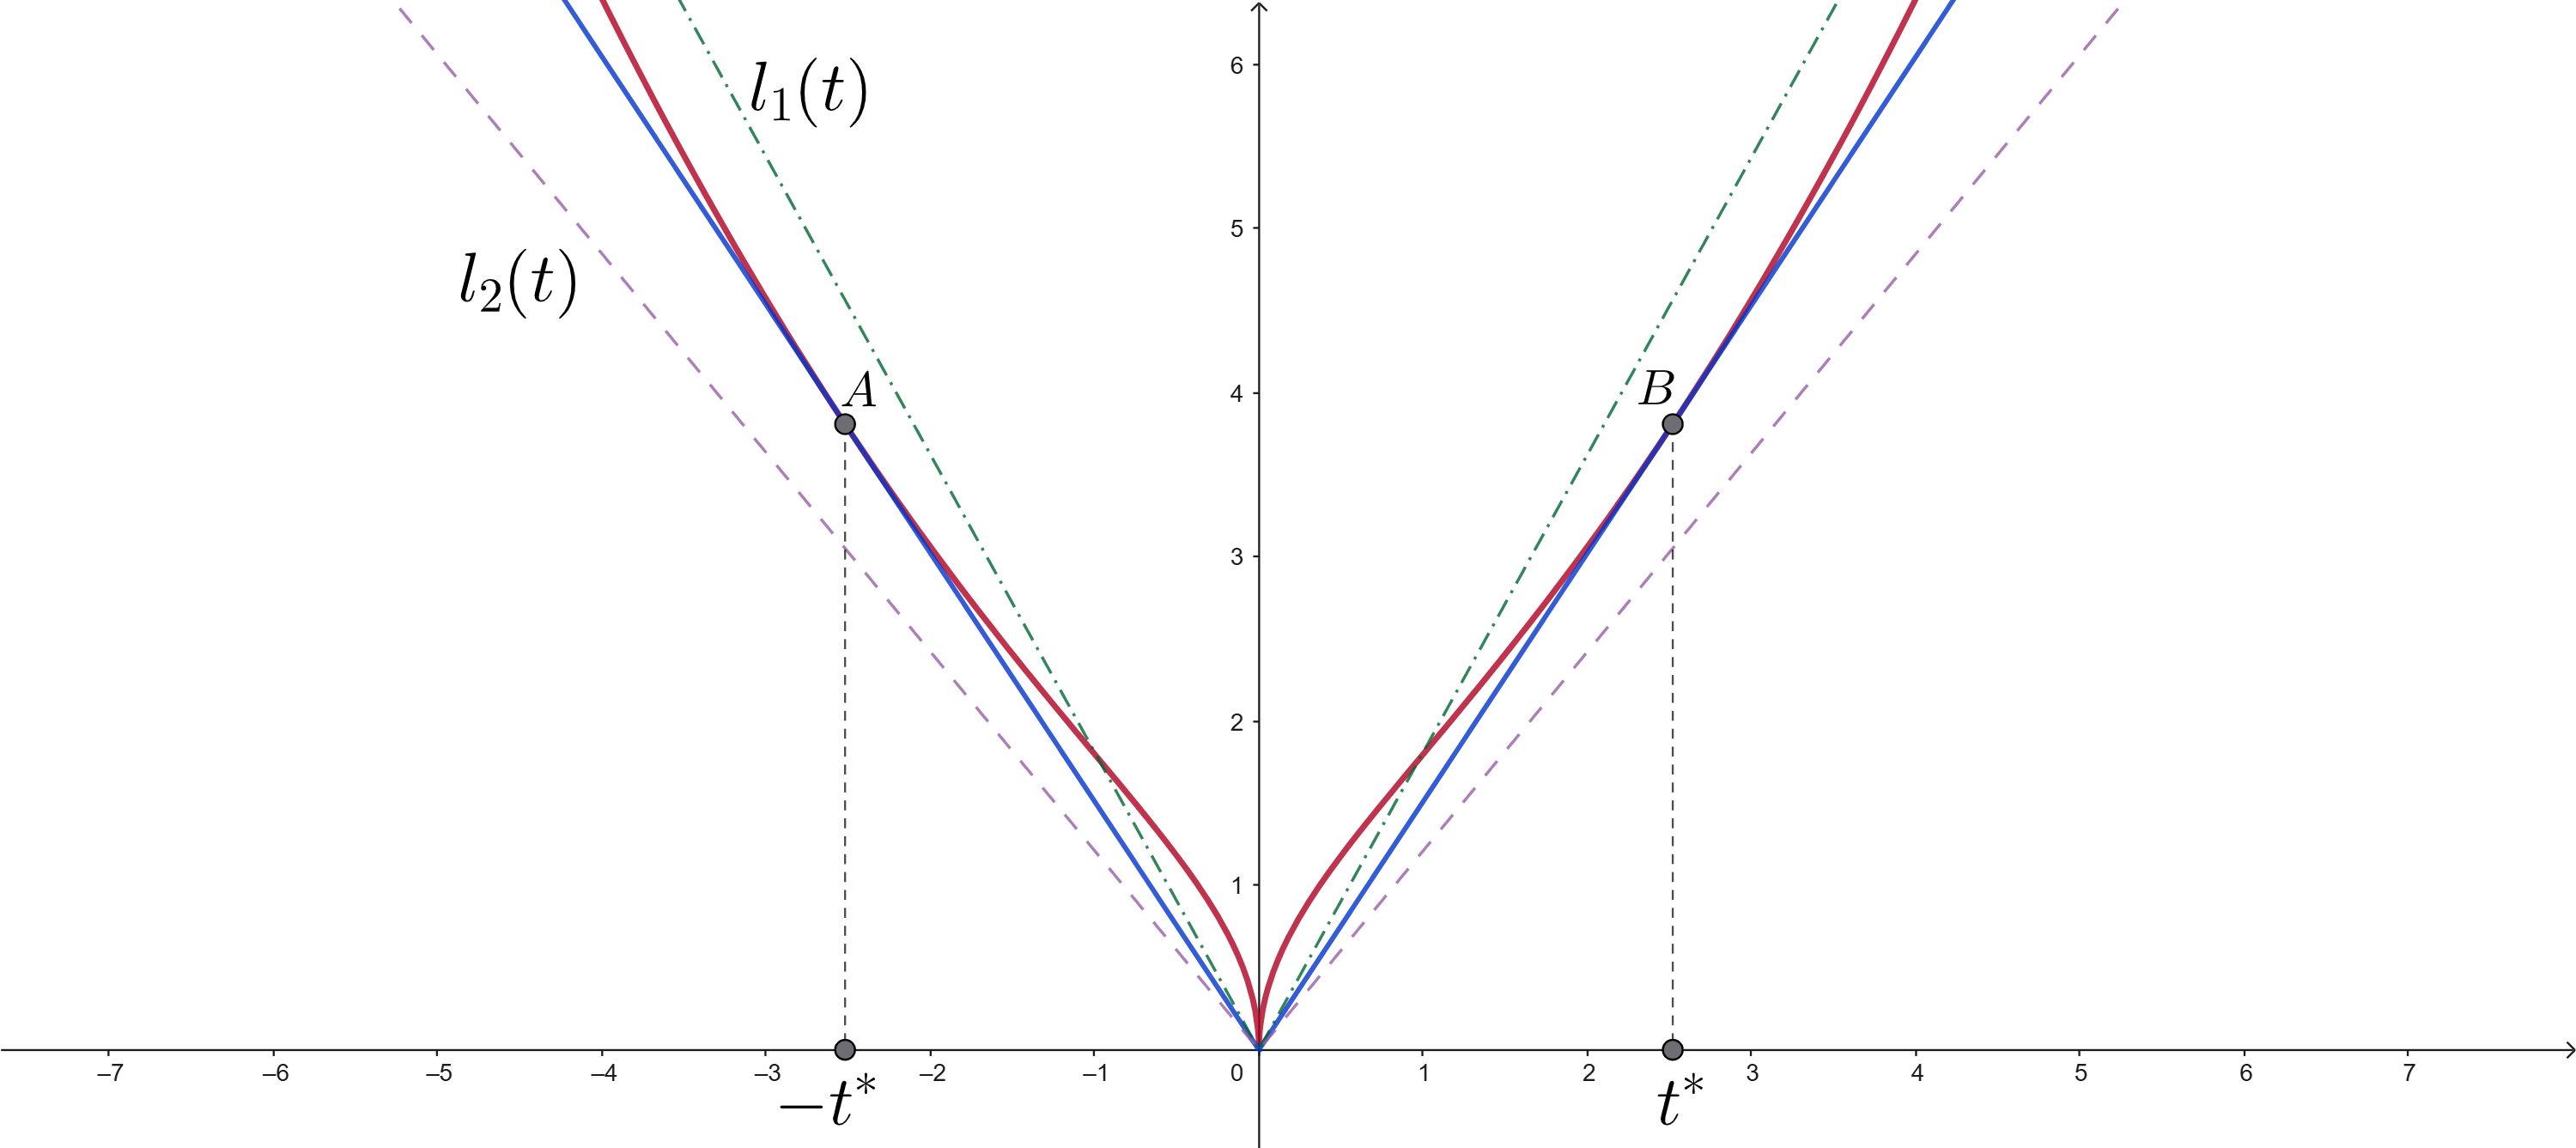
\includegraphics[scale=1]{lqbiconj.png}
     \caption{Graph of the function $\phi_q$ with $q=0.5$, $\alpha=0.4$, $b=1.6$, in red. The two continuous lines in blue represents the greatest continuous affine minorant of $\phi_q$ in $[-t^*, t^*]$. Notice that the points $A$ and $B$ represents the tangency point a which these lines cuts the graph of $\phi_q$. In addition, we see that the two lines $l_1$ and $l_2$ cuts in more that one point the graph of $\phi_q$ (when its slope is greater than $\phi'_q(t^*)$, or is below the blue lines (when its slope is lower than $\phi'(t^*)$.}
     \label{fig:lqbiconj}
 \end{figure}

 \begin{figure}[ht]
     \centering
     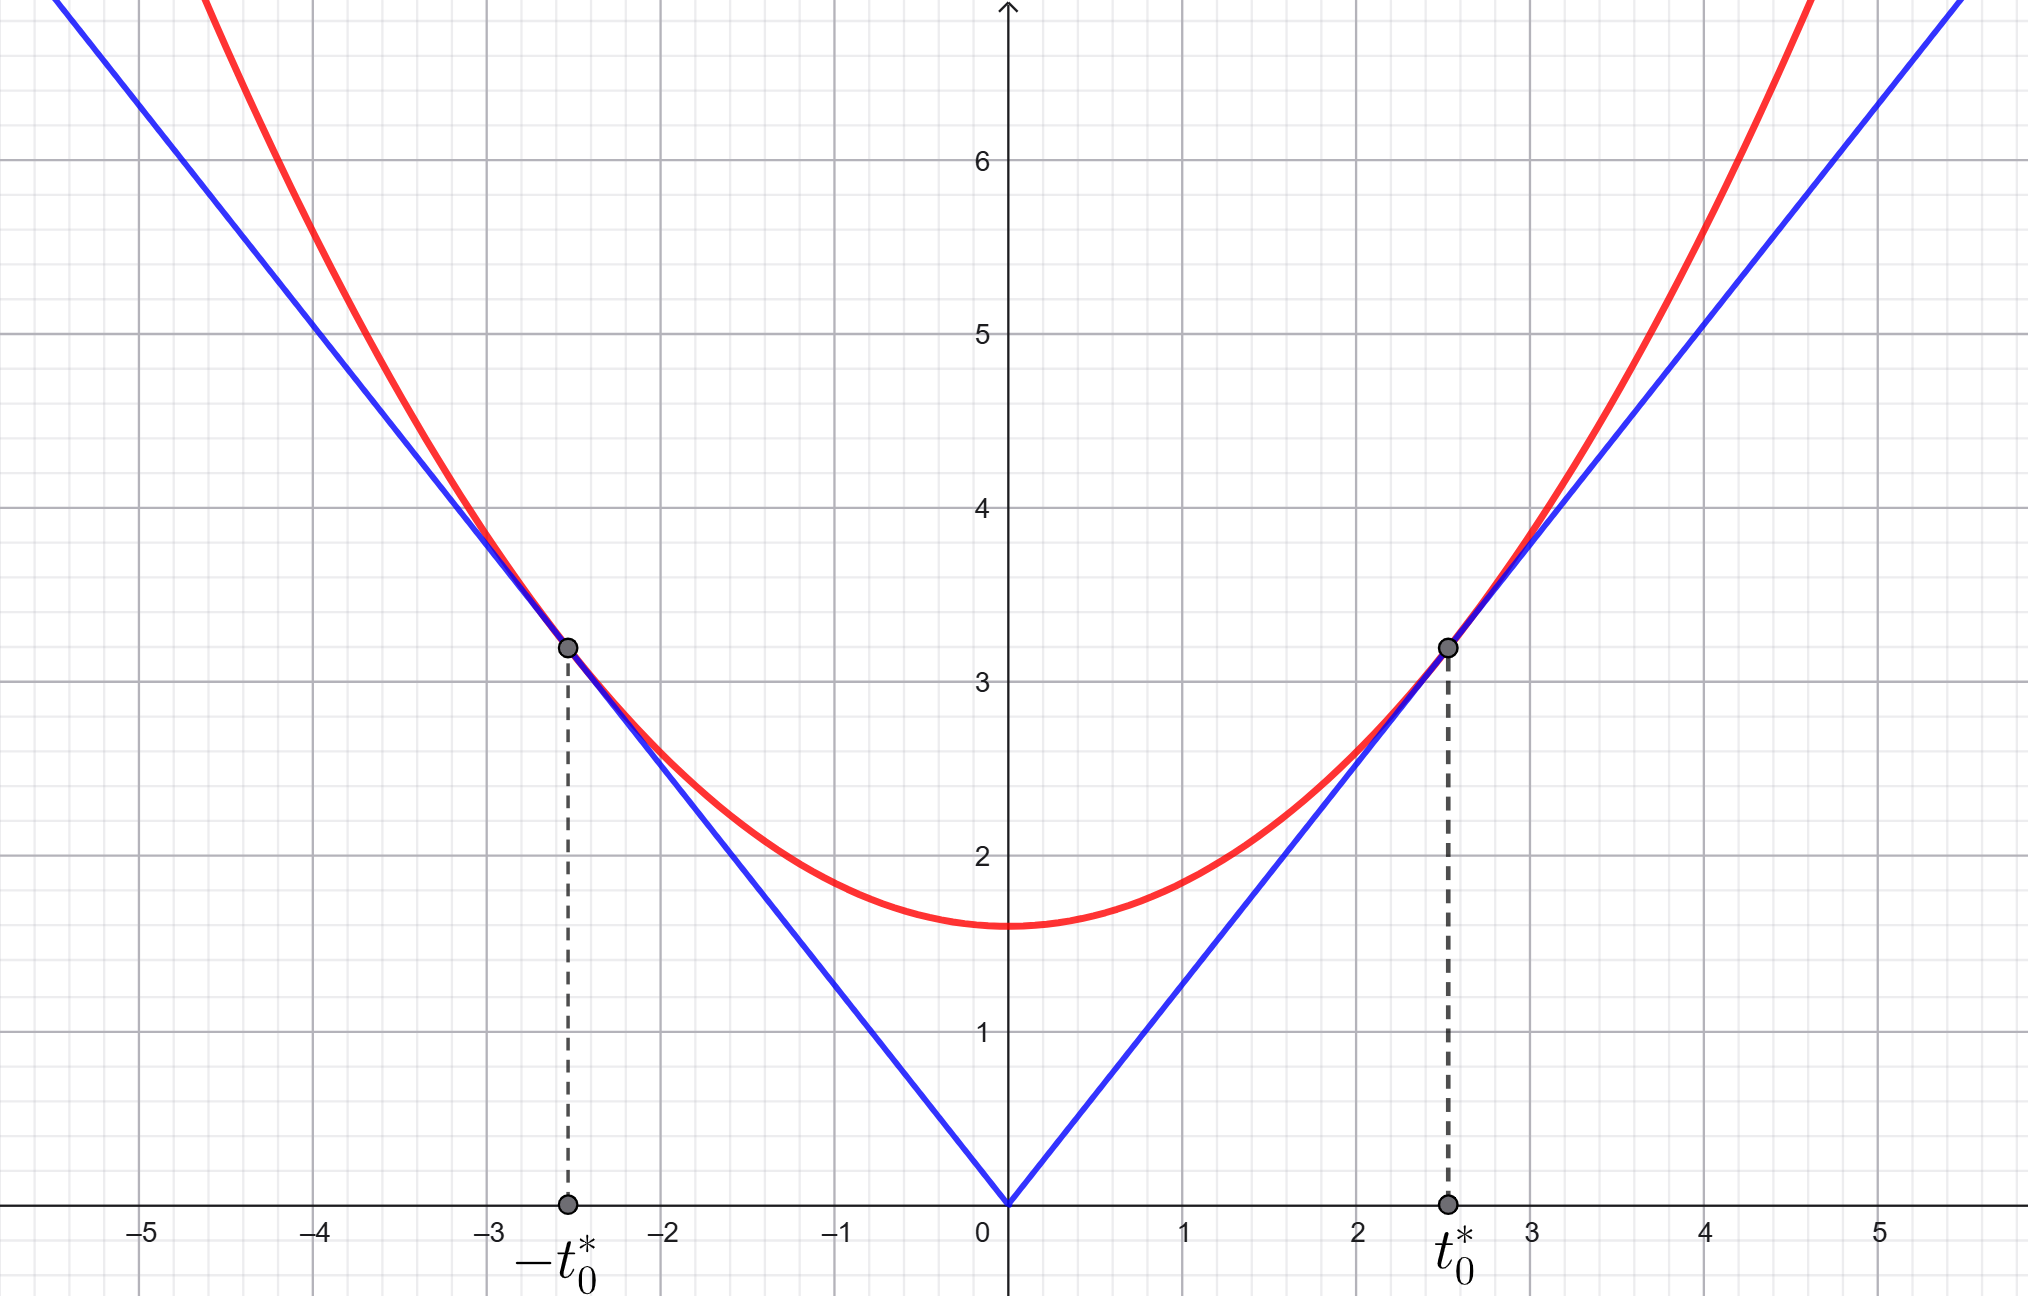
\includegraphics[scale=0.16]{l0biconj.png}
     \caption{Graph of the function $\phi_0$ with $\alpha=0.5$, $b=1.6$, in red. The blue continuous line represents again the greatest affine minorant for $\phi_0$ at $[-t_0^*, t_0^*]$. The construction of the biconjugate for $\phi_0$ is very similar to the case of the biconjugate of $\phi_q$.}
     \label{fig:l0biconj}
 \end{figure}







\section{Numerical algorithms}

In this final section, we present the three numerical algorithms employed to solve the nonconvex optimal control problems investigated in this work. We describe their general structure and report the corresponding convergence results. These methods have proven to be well suited to our framework and have played a key role in validating several theoretical results that were anticipated.

\subsection{The Sequential Quadratic Hamiltonian (SQH) algorithm}

This method is based on the characterization of optimal controls within the framework of the Pontryagin Maximum Principle. Its core idea consists in the iterative solution of a quadratic penalized Hamiltonian constructed from the original optimal control problem. This feature is of particular interest in our setting, since, regardless of the level of penalization imposed on the control, each iteration ultimately reduces to the solution of an optimization problem associated with a quadratic Hamiltonian, that, at least for our studied problems, is equivalent to the solution of unidimensional optimization problems.

Moreover, according to our numerical experiments, this algorithm consistently exhibits the highest robustness and efficiency among the methods considered. Nevertheless, the relatively large number of internal parameters involved introduces a nontrivial tuning challenge. Our experiments reveal that arbitrary or poorly chosen parameter values may lead to unsatisfactory performance, making their careful selection crucial for achieving reliable and accurate results.

The SQH method is not only related to infinite dimensional optimal control problems. In fact, it can be used for solving problems related to ODE's control, differential Nash games, deep learning, stochastics models, and other ones, see \cite{borzi2023}. Even in the theory of optimal control problems governed by PDE's, this method can be used for a large class of these ones, like sparse control problems, state pointwie penalized problems, bilinear problems and more problems. Here, we recall the general framework of the SQH method for control problems governed by elliptic PDE's, and we summarize the results about convergence of the method.

Let $h, g:\mathbb{R}\to [0,\infty)$, $f:\mathbb{R}^3 \to \mathbb{R}$ measurable functions. Consider the problem:

\begin{subequations}\label{eq:sqh_framework_problem}
\begin{equation}
\left\{
\begin{aligned}
\min_{(y,u)\in H_0^1(\Omega)\times L^2(\Omega)} \quad 
& J(y,u) := \int_{\Omega}\big(h(y(x)) + g(u(x))\big)\,dx \\[0.5ex]
\text{s.t.}\quad 
& a(y,v) = \int_{\Omega} f\big(x,y(x),u(x)\big)\,v(x)\,dx,
\quad \forall v \in H_0^1(\Omega), \label{eq:variational_formulation_sqh}\\
& u \in U_{\mathrm{ad}}.
\end{aligned}
\right.
\end{equation}
\end{subequations}




where $a$ is the bilinear operator define in \eqref{eq:bilinear_form}, and $U_{ad}\subset L^2(\om)$. For this kind of problems, we recall the definition of an adjonint state for \eqref{eq:sqh_framework_problem}.A function $p$ is called an adjoint state for \eqref{eq:sqh_framework_problem} if satisfies the equation:
\begin{equation}\label{eq:adjoint_state_sqh}
    a^*(p,z)=\int_{\om}[\partial_y h(y(x))+\partial_y f(x,y(x),u(x))]z(x)\; dx,
\end{equation}
for all $z\in H_0^1(\om)$. Here, $a^{*}$ is the bilinear operator associated to $A^*$ in \eqref{eq:operator_A}.

Since $g,h$ has no more assumptions on their structure, it is possible that \eqref{eq:sqh_framework_problem} have no any solution. However, if we assume that there exist a solution to it, the SQH method demands the following assumptions to guarantee its convergence.
\begin{assumption}\label{assumption:sqh}
    In any compact subset included in the respective domains of definition of
$f$, $h$, and $g$, the following assumptions hold:
\begin{enumerate}
\item
The functions $f$, $\partial_y f$, and $\partial_y h$ are measurable in $x$
and Lipschitz continuous in $y$ and $u$. More precisely, there exist constants
$c_1,c_2,c_3>0$ such that the following inequalities hold uniformly in $x$:
\begin{align*}
|f(x,y_1,u_1)-f(x,y_2,u_2)|
&\le c_1\big(|y_1-y_2|+|u_1-u_2|\big),\\
|\partial_y f(x,y_1,u_1)-\partial_y f(x,y_2,u_2)|
&\le c_2\big(|y_1-y_2|+|u_1-u_2|\big),\\
|\partial_y h(y_1)-\partial_y h(y_2)|
&\le c_3 |y_1-y_2|.
\end{align*}

\item
The solution operators related to the variational formulation  \eqref{eq:variational_formulation_sqh} satisfy the estimates
\[
\|\delta y\|_{L^2(\Omega)} \le c_4 \|\delta u\|_{L^2(\Omega)}, 
\qquad
\|\delta p\|_{L^2(\Omega)} \le c_5 \|\delta u\|_{L^2(\Omega)}.
\]

\item
The adjoint state $p$ which solves the adjoint equation \eqref{eq:adjoint_state_sqh} for given $y$ and $u\in U_{\mathrm{ad}}$
satisfies the uniform bound
\[
\|p\|_{L^\infty(\Omega)} \le c_6.
\]
\end{enumerate}
\end{assumption}
We define the hamiltonian associated to \eqref{eq:sqh_framework_problem} as
\begin{equation}\label{eq:hamiltonian_sqh}
    \mathcal{H}(x,y,u,p):=pf(x,y,u)+h(y)+g(u),
\end{equation}
while the augmented hamiltonian for the SQH is defined as
\begin{equation}
    \mathcal{H}_{\epsilon}(x,y,u,v,p):=\mathcal{H}(x,y,u,p)+\varepsilon (u-v)^2,
\end{equation}
defined for a fixed $\varepsilon>0$. With this augmented hamiltonian, the SQH method is define in Algorithm  \ref{alg:sqh}.

An important feature for ensuring well-definedness of the SQH algorithm is that in step 5. the minimization problem returns a measurable function for all $k=1,2,\cdots$. This fact is not general true for general functions $g, h $ and $f$. However, in our context, we will prove later that our election of $g, h$ produces a sequence of measurable functions $u^k$, given a measurable initial election $u^0$. 

\begin{algorithm}
\caption{Sequential Quadratic Hamiltonian (SQH) method for elliptic optimal control problems}
\label{alg:sqh}
\begin{algorithmic}[1]
\Require Initial control $u^0$, maximal number of iterations $k_{\max}$, tolerance $\kappa>0$, parameters $\tau>0$, $\varepsilon>0$, $\sigma>1$, $\eta>0$, and $\xi\in(0,1)$.
\State Set $k\gets 0$.
\State Compute the state $y^0$ as the solution of 
\[
a(y,v)=\int_{\Omega} f\big(x,y,u^0(x)\big)\,v(x)\,dx,\qquad \forall v\in H_0^1(\om).
\]
\While{$k<k_{\max}$ \textbf{and} $\tau>\kappa$}
    \State Compute $p^k$ as the solution of the adjoint problem:
    \[
    a^*(p,v)=\int_{\Omega}\Big(\partial_y h\big(y^k(x)\big)
    +\partial_y f\big(x,y^k(x),u^k(x)\big)\,p(x)\Big)\,v(x)\,dx,
    \qquad \forall v\in H_0^1(\om).
    \]
    \State For a.e. $x\in\Omega$, determine $u^{k+1}(x)\in U_{\mathrm{ad}}$ such that
    \[
    u^{k+1}(x)\in\arg\min_{w\in U_{\mathrm{ad}}} \mathcal{H}_{\varepsilon}\big(x,y^k(x),w,u^k(x),p^k(x)\big).
    \]
    \State  Compute $y^{k+1}$ as the solution of
    \[
    a(y,v)=\int_{\Omega} f\big(x,y,u^{k+1}(x)\big)\,v(x)\,dx,\qquad \forall v\in H_0^1(\om).
    \]
    \State Compute $\tau \gets \|u^{k+1}-u^k\|_{L^2(\Omega)}^2$.  
    \If{$J\!\left(y^{k+1},u^{k+1}\right) - J\!\left(y^k,u^k\right) > -\eta\,\tau$}
        \State Increase $\varepsilon \gets \sigma\,\varepsilon$ and \textbf{go to} Step 2.
    \ElsIf{$J\!\left(y^{k+1},u^{k+1}\right) - J\!\left(y^k,u^k\right) < -\eta\,\tau$}
        \State Decrease $\varepsilon \gets \xi\,\varepsilon$.
    \EndIf
    \State Update $k\gets k+1$.
\EndWhile
\end{algorithmic}
\end{algorithm}
The next result establish a minimising property for the SQH algorithm. This result can be found in \cite[Theorem 7.3]{borzi2023}

\begin{theorem}\label{thm:sqh_minimizing}
Let $(y^k,u^k)$ and $(y^{k+1},u^{k+1})$ be generated by the SQH method,
Algorithm~\ref{alg:sqh}, and let $u^{k+1}$ and $u^k$ be measurable.
Assume that Assumption~\ref{assumption:sqh} hold.
Then, there exists $\theta>0$, independent of $\varepsilon$, $k$, and $u^k$,
such that for the parameter $\varepsilon>0$ currently chosen by
Algorithm~\ref{alg:sqh}, the following estimate holds:
\begin{equation}\label{eq:sqh_descent}
J\big(y^{k+1},u^{k+1}\big) - J\big(y^k,u^k\big)
\le -(\varepsilon-\theta)\,\|u^{k+1}-u^k\|_{L^2(\Omega)}^2 .
\end{equation}
In particular, it holds that
\[
J\big(y^{k+1},u^{k+1}\big) - J\big(y^k,u^k\big)
\le -\eta\,\tau
\quad \text{for } \varepsilon \ge \theta+\eta,
\]
where
\[
\tau := \|u^{k+1}-u^k\|_{L^2(\Omega)}^2 .
\]
\end{theorem}

Finally, we provide the result of convergence for this Algorithm. The proof of this one can be found in \cite[Theorem 7.4]{borzi2023}
\begin{theorem}\label{thm:sqh_convergence}
Let the assumptions of Theorem~\ref{thm:sqh_minimizing} be fulfilled.
Assume that in Algorithm~\ref{alg:sqh}, at every $k$-th iterate,
the parameter $\varepsilon=\theta+\eta$ is chosen.
Then, the following statements hold:
\begin{enumerate}[label=\textup{(\alph*)}]
\item
The sequence $\big(J(y^k,u^k)\big)_{k=0,1,2,\dots}$ is monotonically decreasing
and converges to some value
\[
\hat J \ge \inf_{u\in U_{\mathrm{ad}}} \hat J(u).
\]

\item
It holds that
\[
\lim_{k\to\infty} \|u^{k+1}-u^k\|_{L^2(\Omega)} = 0.
\]
\end{enumerate}
\end{theorem}

\subsection{The Difference of Convex functions (DC) algorithm}

The theory of Difference of Convex  (DC) functions was developed in the later 70's by Toland first, and Singer \cite{toland, singer}, in the context of convex maximization theory in finite dimensional spaces. Later, several deep results and algorithms based on this theory was proposed by Pham Dinh Tao and Le Thi Hoai An in \cite{tao}. Inspired by this work, the infinite dimensional case for finding existence of solutions, necessary and sufficient optimal conditions of DC problems in the context of indefinite quadratic problems are deveolped in \cite{bonnans, yen}. The later novelty paper \cite{lim} deals with DC algorithms in general Hilbert spaces, proving sufficient conditions for the convergence of this algorithm and given a rate of convergence for indefinite quadratic programs. 

One of the most appealing features of DC algorithms lies in the formulation and solution of two primal–dual problems, for which a wide range of numerical methods have been extensively studied and optimized. In the context of nonconvex optimal control problems, several works have addressed this approach; see, for instance, \cite{hinze, ioffe}. For optimal control problems involving $L^q$-type penalizations, the work \cite{merino2019} is particularly relevant. There, a Huber-type regularization is introduced to incorporate the nonconvex penalty, and by expressing the cost functional as the difference of two convex functions, a DC scheme based on two primal–dual problems is developed. One of these subproblems involves an $L^1$-penalized optimal control problem, for which a variety of efficient numerical solution methods are available.
We consider the general setting of the DC algorithm. For a general Hilbert space $X$, let $g, h: X\to \mathbb{R}$ two convex and lower semicontinuous functions. Consider the minimization problem
\begin{equation}\label{eq:dc_formulation}
    \inf_{x\in X} f(x):=g(x)-h(x).
\end{equation}
\eqref{eq:dc_formulation} is called a DC program. Associated with this problem, we formulate the dual problem associated to it as
\begin{equation}\label{eq:dc_dual_formulation}
    \inf_{x\in X} \widetilde{f}(x):=h^{*}(x)-g^{*}(x).
\end{equation}
It can be shown that \eqref{eq:dc_formulation} and \eqref{eq:dc_dual_formulation} has the same optimal value, see \cite[Proposition 2.5]{lim}. Moreover, the following first order optimally condition, whcih is important for developing the DC algorithm, follows.
\begin{proposition}\label{prop:first_order_condition_dc}
    If $x^*$ is a local solution for \eqref{eq:dc_formulation}, then $\partial h(x^*)\subset \partial g(x^*)$.
\end{proposition}

The following algorithm is called the DC algorithm. 

\begin{algorithm}[ht]
\caption{DC Algorithm (DCA) in Hilbert spaces}
\label{alg:dca}
\begin{algorithmic}[1]
\Require DC decomposition $F = g - h$, where $g,h : X \to \mathbb{R}\cup\{+\infty\}$ are proper, lower semicontinuous, convex functions.
\Require Initial point $x^0 \in \operatorname{dom} g$.
\State Set $k \gets 0$.
\While{stopping criterion not satisfied}
    \State
    Choose $y^k \in \partial h(x^k)$, provided that $\partial h(x^k)\neq \emptyset$.
    \State 
    Choose $x^{k+1} \in \partial g^*(y^k)$, provided that $\partial g^*(y^k)\neq \emptyset$.
    \State Update $k \gets k+1$.
\EndWhile
\end{algorithmic}
\end{algorithm}
Before to establish the properties of the DC algorithm, we introduce the concept of modulus of convexity. 
\begin{definition}\label{def:modulus_convexity}
    Lef $f:X\to \mathbb{R}$ a convex function. Its modulus of convexity is defined as
    \[
    \rho(f)=\sup \l\{\rho\ge 0: f(\cdot)-\frac{\rho}{2}\norm{\cdot}^2 \mbox{ is a convex function over }X \r\}
    \]
\end{definition}

Consider the pair of problems \eqref{eq:dc_formulation} and \eqref{eq:dc_dual_formulation}. If $\rho(g) > 0$ 
(resp., $\rho(g^*) > 0$), let $\rho_1$ (resp., $\rho_1^*$) be a real number such that
\[
0 \le \rho_1 < \rho(g) \quad (\text{resp., } 0 \le \rho_1^* < \rho(g^*)).
\]
If $\rho(g) = 0$ (resp., $\rho(g^*) = 0$), let $\rho_1 = 0$ (resp., $\rho_1^* = 0$).
If $\rho(h) > 0$ (resp., $\rho(h^*) > 0$), let $\rho_2$ (resp., $\rho_2^*$) be a real number such that
\[
0 \le \rho_2 < \rho(h) \quad (\text{resp., } 0 \le \rho_2^* < \rho(h^*)).
\]
If $\rho(h) = 0$ (resp., $\rho(h^*) = 0$), let $\rho_2 = 0$ (resp., $\rho_2^* = 0$). Finally, define
\[
d x^k := x^{k+1} - x^k, \qquad d y^k := y^{k+1} - y^k,
\]
and denote the optimal value of \eqref{eq:dc_formulation} by $\alpha$, that is,
\[
\alpha := \inf \{ f(x) = g(x) - h(x) : x \in H \}.
\]
The following Theorem establishes the convergence properties of the DC algorithm. Its proof can be found in \cite[Theorem 2.11]{lim}.
\begin{theorem}\label{thm:convergence_dc}
Assume that the iteration sequences $(x^k)$ and $(y^k)$ are generated by the DCA. We have
\begin{enumerate}
\item[(i)]
\begin{align*}
(g - h)(x^{k+1})
&\le (h^* - g^*)(y^k)
- \max \left\{ \frac{\rho_2}{2} \|d x^k\|^2, \frac{\rho_2^*}{2} \|d y^k\|^2 \right\} \\
&\le (g - h)(x^k)
- \max \Bigg\{
\frac{\rho_1 + \rho_2}{2} \|d x^k\|^2,\,
\frac{\rho_1^*}{2} \|d y^{k-1}\|^2 \\
&\hspace{3cm}
+ \frac{\rho_2}{2} \|d x^k\|^2
+ \frac{\rho_1^*}{2} \|d y^{k-1}\|^2
+ \frac{\rho_2^*}{2} \|d y^k\|^2
\Bigg\}.
\end{align*}

\item[(ii)]
\begin{align*}
(h^* - g^*)(y^{k+1})
&\le (g - h)(x^{k+1})
- \max \left\{ \frac{\rho_1}{2} \|d x^{k+1}\|^2, \frac{\rho_1^*}{2} \|d y^k\|^2 \right\} \\
&\le (h^* - g^*)(y^k)
- \max \Bigg\{
\frac{\rho_1^* + \rho_2^*}{2} \|d y^k\|^2,\,
\frac{\rho_1}{2} \|d x^{k+1}\|^2 \\
&\hspace{3cm}
+ \frac{\rho_2}{2} \|d x^k\|^2
+ \frac{\rho_1^*}{2} \|d y^k\|^2
+ \frac{\rho_2}{2} \|d x^k\|^2
\Bigg\}.
\end{align*}

\item[(iii)]
If $\alpha$ is finite, then $\{(g-h)(x^k)\}$ and $\{(h^*-g^*)(y^k)\}$ are decreasing sequences that converge to the same limit $\beta \ge \alpha$.

\item[(iv)]
Assume that $\alpha$ is finite and that $(x^k)$ and $(y^k)$ are bounded.  
If $\{x^k\}$ contains a strong limit point $x^*$ (resp., $(y^k)$ contains a strong limit point $y^*$), then there is a weak limit point $y^*$ of $\{y^k\}$ (resp., $x^*$ of $\{x^k\}$) such that
\[
(x^*, y^*) \in [\partial g^*(y^*) \cap \partial h^*(y^*)]
\times
[\partial g(x^*) \cap \partial h(x^*)].
\]

Moreover, if $\rho_1 + \rho_2 > 0$ (resp., $\rho_1^* + \rho_2^* > 0$), then
\[
(g - h)(x^*) = (h^* - g^*)(y^*) = \beta.
\]
\end{enumerate}
\end{theorem}





\subsection{The Semismooth Newton (SSN) algorithm}

The semismooth Newton (SSN) method is formulated within the framework of solving optimization problems 
of the form

\begin{equation}
\min_{y,u\in U\times Y} J(y,u)
\quad \text{subject to } E(y,u)=0 \text{ and } g(y,u) \in C.
\end{equation}


where $U$ and $Y$ denote the control and state spaces, respectively. Here, $J$ represents a cost functional, 
$E$ denotes a partial differential equation linking the control $u$ and the state $y$, and $g(y,u)\in C$ 
represents a generic inequality-type constraint. The mapping $g$ takes values in a vector of $m$ measurable 
real-valued functions, while $C\subset \mathbb{R}^{m}$ is a closed and convex set.
The goal of the method is to reformulate the stated problem, starting from first-order necessary optimality 
conditions, into an equivalent system of equations of the form $F(u)=0$, where $F$ must be a semismooth 
function—a concept that will be detailed later.

As pointed out in \cite{ulbrich}, the method was originally designed to address problems of this type in 
finite-dimensional spaces. Some early contributions in this direction can be found in \cite{mifflin, qi, pang}, 
with \cite{mifflin} being the first work to introduce the concept of semismoothness in finite-dimensional 
settings. Extensions of several concepts from the theory of semismooth operators to Banach spaces were later 
developed in works such as \cite{kummer, robinson, chen}. However, in \cite{ulbrich}, the use of superposition 
operators makes it possible to transfer many essential features of semismooth Newton methods from 
finite-dimensional spaces to general Banach spaces.

The SSN method has been widely applied to optimal control problems governed by linear elliptic partial 
differential equations and penalized with an $L^1$ term. In \cite{stadler}, it is shown that, under a 
reformulation of the problem via a semismooth function, the method converges superlinearly, provided that 
the initial iterate is sufficiently close to the solution. The convexity of the problem and the coercivity 
of the differential operator play a fundamental role in establishing the convergence of the method. 
In \cite{merino2021}, a direct application of the method is presented for problems involving $L^q$
 penalization, with $q\in (0,1)$. A Huber-type regularization is introduced in order to show that the 
 problem can be reformulated through a semismooth Newton function. However, no convergence proof of the 
 method is provided therein.

A generalization of Stadler’s analysis to problems governed by semilinear partial differential equations 
is studied in \cite{casasmateos}. Nevertheless, the convergence proof in this setting requires the 
development of second-order optimality conditions. For linear problems with $L^q$ penalization, one may 
follow a combination of methods based on the results presented in \cite{stadler} and \cite{casasmateos}. 
Hoever, a possible estension to the semilinear case is particularly difficult, since there exists only
second order conditions like the presented in \cite{casas-wachsmuth}, which not implies directly enough 
conditions to establish the convergence of the method.

Before the introduction of the SSN algorithm, we present the definition of a semismooth function.

\begin{definition}\label{def:semismooth}
Let $X$ and $Y$ be Banach spaces, and let $V \subset X$ be an open set.
Let $f : V \to Y$ and
\[
\partial^* f : V \rightrightarrows \mathcal{L}(X,Y)
\]
be a set-valued mapping such that $\partial^* f(y) \neq \emptyset$ for all $y \in V$.
We say that $f$ is $\partial^*$-semismooth at $y \in V$ if $f$ is continuous at $y$ and
\[
\sup_{M \in \partial^* f(y+s)}
\| f(y+s) - f(y) - Ms \|_{Y}
= o(\|s\|_{X})
\quad \text{as } \|s\|_{X} \to 0.
\]
Moreover, we say that $f$ is $\alpha$-order $\partial^*$-semismooth at $y$, $0 < \alpha \le 1$,
if $f$ is continuous near $y$ and
\[
\sup_{M \in \partial^* f(y+s)}
\| f(y+s) - f(y) - Ms \|_{Y}
= O(\|s\|_{Y}^{1+\alpha})
\quad \text{as } \|s\|_{X} \to 0.
\]
\end{definition}

Now, assume that $f:V\subset X\to Y$ is a $\partial^*$-semismooth function. 
We are interested in solving the equations
\begin{equation}\label{eq:ssn_equation}
f(y)=0.
\end{equation}
The following algorithm, called SSN algorithm, is implemented in order to find the root of $f$ as 
shown in the last equation stablish. We assume that $Y$ is continuously
and densely embedded in a bigger space $Y_0$.

\begin{algorithm}[ht]
\caption{Semismooth Newton method}
\label{alg:ssn_ulbrich}
\begin{algorithmic}[1]
\State Choose an initial point $y_0 \in V$ and set $k = 0$.
\While{stopping criterion not satisfied}
\State Choose $M_k \in \partial^* f(y_k)$ and compute $s_k \in Y_0$ from
\[
M_k s_k = - f(y_k).
\]
\State Set $y_{k+1}^{0} = y_k + s_k$.
\State Perform a smoothing step: $Y_0 \ni y_{k+1}^{0} \mapsto y_{k+1} = S_k\!\left(y_{k+1}^{0}\right) \in Y$.
\If{$y_{k+1} = y_k$}
\State \textbf{stop} with result $y^* = y_{k+1}$.
\EndIf
\State $k \gets k+1$.
\EndWhile
\end{algorithmic}
\end{algorithm}

The following assumption is crucial for the convergence of the SSN algorithm.
\begin{assumption}\label{ass:ulbrich_3_12}
The space $Y$ is continuously and densely embedded in a Banach space $Y_0$ such that:
\begin{enumerate}
\item[(a)] \emph{(Regularity condition)}  
The operators $M_k$ map $Y_0$ continuously into $Z$ with bounded inverses, and there exists a constant
$C_{M^{-1}} > 0$ such that
\[
\|M_k^{-1}\|_{\mathcal{L}(Z,Y_0)} \le C_{M^{-1}}.
\]

\item[(b)] \emph{(Smoothing condition)}  
The smoothing steps in step 5 satisfy
\[
\|S_k(y_{k+1}^0) - \bar y\|_Y \le C_S \|y_{k+1}^0 - \bar y\|_{Y_0}
\]
for all $k$, where $\bar y \in Y$ solves~(3.7).
\end{enumerate}
\end{assumption}

Under this Assumption, the following Theorem follows. For a proof 
of this result, see \cite[Theorem 3.13]{ulbrich}

\begin{theorem}\label{thm:ssn_convergence}
Let $f : Y \supset V \to Z$ be an operator between Banach spaces defined on the open set $V$,
with generalized differential $\partial^* f : V \rightrightarrows \mathcal{L}(Y,Z)$.
Denote by $\bar y \in V$ a solution of \eqref{eq:ssn_equation} and let Assumption~\ref{ass:ulbrich_3_12} hold.
Then the following assertions are valid:
\begin{enumerate}
\item[(a)]
If $f$ is $\partial^*$-semismooth at $\bar y$, then there exists $\delta > 0$ such that,
for all $y_0 \in \bar y + \delta B_Y$,
Algorithm \ref{alg:ssn_ulbrich} either terminates with $y^* = y_k = \bar y$ or generates a sequence
$(y_k) \subset V$ that converges $q$-superlinearly to $\bar y$ in $Y$.

\item[(b)]
If in~(a) the mapping $f$ is $\alpha$-order $\partial^*$-semismooth at $\bar y$,
$0 < \alpha \le 1$, then the $q$-order of convergence is at least $1+\alpha$.
\end{enumerate}
\end{theorem}

%\chapter{Nonconvex optimal control problems with $L^q$ penalizations}

	
	\section{Penalties of the form $\int_{\om}|u|^q$ with $q\in [0,1)$}
		Optimal control problems with nonconvex $L^q$-quasinorms (with $q \in (0,1)$) can be regarded as a regularization of the so called $L^0$ sparse penalized problems, in which the optimal control fulfills a minimal support's volume criterion, promoted by the $L^0$ penalizer, see \cite{ito-kunisch2014, wachsmuth2011}.  However, depending on the regulization parameters present in the cost function,optimal controls induced by the  $L^q$-quasinorm entail subtle jump discontinuities and sparse properties that differs from those optimal controls generated by the $L^0$-pseudo norm; for instance, $L^q$ optimal controls may have smaller supports and, moreover, jump discontinuities may be not monotone, see Figure \ref{fig:jump}. These properties are relevant for optimal control as they enhance the sparsity and jump discontinuities characterization of the optimal controls.
	
	Optimal controls induced by $L^q$-quasinorm penalizers share similarities with those induced by $L^1$-norm and by the $L^0$ penalizer. It is well known that these controls tend to have small supports depending on the sparse regularization cost \cite{stadler2006}. However, a simple but essential difference in considering $L^q$-quasinorms is that jump discontinuities appear at the boundary of optimal control's support. This feature is potentially advantageous in several applications. 
	In particular, the sparsification effect induced by these penalizers are useful in applications requiring a sharp localized action of the control within the domain, which is crucial for instance, to reduce the cost of the tracking term, see \cite{casas}.  Other examples arising from inverse sparse reconstruction problems and image-processing-related applications can benefit from solutions with jump discontinuities. For instance, in imaging, the so called $TV^q$ penalizer enforces certain graphical features. 
	
	
 	Research on optimal control problems with $L^q$-quasinorm penalizers is recent.  Perhaps, the biggest recognizable difficulty in considering the $L^q$-quasinorm is the lack of convexity (a fortiori, the lack of weak lower semicontinuity) of the penalizer. Therefore, analyzing the existence of a solution such as developing efficient numerical algorithms are challenging tasks. In \cite{ito-kunisch2014}, the $L^0$ penalization was studied along with the $L^q$-quasinorm penalizer. In the last case,  a penalty given by the $L^2$-norm of the gradient was added to the cost, which allows compactness arguments to guarantee the existence of solutions in $H^{1}$. However, the gradient cost term removes the jump discontinuities from solutions, which is a relevant feature of the $L^q$-quasinorm. 
	
	The associated optimality conditions were derived in \cite{ito-kunisch2014} utilizing a $\rm{C}^1$ regularization of the nonconvex term. Furthermore,  \cite{merino2019} derived an optimality system by regularizing the cost with a continuous nonconvexity, and thereafter, the subsequent application of the difference-of-convex programming, including control constraints in the case of linear elliptic second-order PDEs. In both cases, the optimality conditions depend on a regularization parameter that is taken to a limit to characterize the optimality conditions of the original problem.
	
 	
In this paper, we investigate an optimal control problem subject to a linear second-order elliptic partial differential equation.	The cost function  $J: L^2(\om) \times (\om) \to \reals$ involving an $L^q$--quasinorm ($q\in (0,1)$) penalization, is given by
	\begin{equation}\label{eq:cost_q}
		\displaystyle J{(y,u)}= ~\frac{1}{2}\| y-y_d \|^2_{L^2(\om)}+\frac{ \alpha}{2}\|u\|^2_{L^2(\om)}+\beta \int_\om |u|^{q} dx.
	\end{equation}

We formulate the following distributed optimal control problem using the objective functional \eqref{eq:cost_q} as follows:
	\begin{equation}
		\tag{$P$} \label{eq:OCP}
		\begin{cases}
			\displaystyle\min_{(y,u)} J(y,u)\\
			\hbox{ subject to: }\\
			\hspace{40pt}\begin{array}{rll}
				A y=&u + f, &\hbox{in  } \om, \\
				y=&0, &\hbox{on  }  \Gamma.
			\end{array}			
		\end{cases}
	\end{equation}
	In our setting, $\om \subset \reals^n$ is a bounded Lipschitz domain, and $y_d$ and $f$ are given functions in $L^2(\om)$.
	Moreover, $A$ is a uniformly elliptic second--order differential operator of the form:
	\begin{equation}\label{eq:A}
		(Ay) (x) = - \sum_{i,j=1}^n \frac{\partial}{\partial x_i}	\l( a_{ij}(x)\frac{\partial y(x)} {\partial x_j }\r) +c_0 y(x),
	\end{equation}
	%
	with coefficients $a_{ij}$ in $\rm{C}^{0,1}(\bar\om)$, and $c_0\geq 0$ in $L^{\infty}(\om)$. In addition, the matrix $(a_{ij})$ is symmetric and fulfills the uniform ellipticity condition: 
	\begin{equation}\label{eq:uelliptic}
		\exists\, \sigma>0 : \quad   \sum_{i,j=1}^n a_{ij}(x) \xi_i\xi_j \geq \sigma |\xi|^2, \quad \forall \xi \in \reals^n, \text{for almost all } x \in \om. 	
	\end{equation}  	

	
	\emph{Our contribution.} Here, we highlight the key contributions of this paper.
	\begin{itemize}
		\item We proved the existence of (generalized) optimal controls  $L^2$ for the $L^q$-quasinormed ($q\in(0,1)$) optimal control problems, by defining a thresholding operator, and extending the result for $L^0$-pseudonorm penalized optimal controls given by Ito and Kunisch \cite{ito-kunisch2014}.
		%\item We provide a novel approximation result for the solutions of $L^q$-quasinorm optimal controls to $L^0$-pseudonorm optimal controls in terms of $\|\bar u_0 - \bar u_q\|_{L^2(\om)}$.
		\item We introduced a \emph{Sequential Quadratic Hamiltonian} method (SQH) for solving \eqref{eq:OCP}, satisfying hypotheses for convergence.
		\item We provide an error analysis for the variational discretization approach using the finite-element method for problem \eqref{eq:OCP}. 
  \item We develope some numerical tests illustrating the associated theory.
	\end{itemize}
	 	
	
	\emph{Organization of the paper.}  We begin by deriving an optimality system in Section 2, for which we analyze its solvability and, subsequently, deduce the existence of the optimal controls. The box-constrained case is briefly discussed at the end of this section. In section 3, we formulate the \emph{Sequential Quadratic Hamiltonian} method for solving the optimal control problem.  We show the algorithm's performance thorough numerical tests. Section 4 is devoted to the variational finite-element approximation of the optimal control problem. Several convergence results and error estimates are discussed. This analysis is followed by several numerical experiments aiming to provide insight into the approximation behavior of the solutions. Finally, we draw conclusions from our findings.
	
	
	\section{Existence of solution and optimality conditions }
    \section{Problem formulation}
    \section{Partial convexification of the $L^q$ terms}
    \section{ The Maximum Principle and its equivalence with the Partial convexification of the problem}
    \section{Incoporating control constrains}
    \section{Incorporating mixed control-state cosntrains}
    
	We argue for the existence of a solution to problem \eqref{eq:OCP}, following the methodology presented in \cite{ito-kunisch2014}, where the authors demonstrated the existence of a solution using the $L^0$-pseudonorm as a penalizer in the cost function. We proceed by first deriving the first-order necessary optimality conditions that characterize solutions to \eqref{eq:OCP}. Then, after obtaining a solution to these conditions, we will verify that it is, indeed, a global minimum for \eqref{eq:OCP}.

We denote by $a(\cdot, \cdot):H_{0}^{1}(\om) \times H_{0}^{1}(\om)\to \reals$  the bilinear form associated to the second-order differential operator $A$, defined by $$a(y,v)=\int_\om a_{ij}(x)\frac{\partial y(x)}{\partial x_i} \frac{\partial v(x)}{\partial x_i} dx + \int_\om c_0(x)\,y(x)v(x)\,dx, $$
while $a^*$ denotes the corresponding bilinear operator associated to $A^*$.
	
	Thanks to the Lax--Milgram theorem and the elliptic regularity \cite{brezis2010}, we know that for every $w \in L^2(\om)$ there exist $y\in H_{0}^{1}(\om)$ and a positive constant $c_a>0$, satisfying: 
	\begin{subequations}\label{eq:state_formul}
		\begin{align}
			&a(y,v) = (w,v)_{L^2(\om)}, \quad \forall v \in H_{0}^{1}(\om),\label{eq:state}\\
			&\norm{y}_{H_{0}^{1}(\om)} \leq c_a\norm{w}_{L^2(\om)}. \label{eq:state_continuity}
		\end{align}
	\end{subequations}
 The same is true for the adjoint problem:
	\begin{subequations}
		\begin{align}
			&a^*(z,v) = (w,v)_{L^2(\om)}, \quad \forall v \in H_{0}^{1}(\om),\label{eq:state*}\\
			&\norm{z}_{H_{0}^{1}(\om)} \leq c_a^*\norm{w}_{L^2(\om)}\label{eq:esti_state*}.
		\end{align}
	\end{subequations}
for some positive constant $c_a^*$.

Furthermore, thanks to Theorem 4.4 in \cite{stampacchia1965} and the continuous injection $L^2(\om) \hookrightarrow W^{-1,p}(\om)$, we have that, for a fixed $p>n$, there exists a linear and continuous operator $S:L^2(\om)\to L^{\infty}(\om)\cap H_{0}^{1}(\om)$, which assigns any $w\in L^2(\om)$  the corresponding state $y$  satisfying \eqref{eq:state} with $w$ as right-hand side. The continuity of $S$ also implies the existence of a constant $c_{\infty}>0$ such that the solution $y=Sw$ of \eqref{eq:state} satisfies
\begin{equation}\label{eq:esti_state_uniform}
    \norm{y}_{L^{\infty}(\om)}\le c_{\infty}\norm{w}_{L^2(\om),}
\end{equation}
Analogously, for the solution $z$ of \eqref{eq:state*} it holds that 
\begin{equation}\label{eq:esti_state*_uniform}
    \norm{z}_{L^{\infty}(\om)}\le c_{\infty}\norm{w}_{L^2(\om),}
\end{equation}
for some constant $c_{\infty}^*>0$. We denote by $S^*:L^2(\om)\to L^{\infty}(\om)\cap H_{0}^{1}(\om)$ the corresponding solution operator that for any $w\in L^2(\om)$ assigns the  solution $z=S^*(w)$ of \eqref{eq:state*}.

	\subsection{Optimality conditions}	
	
	
	The adjoint state is an essential tool to represent optimality conditions. Given a control $u \in L^2(\om)$ with associated state $y\in H_{0}^{1}(\om)$, we introduce the adjoint state $\varphi$ as the solution of the following variational problem, which can be in the same way as problem \eqref{eq:state}: 
	\begin{align}\label{eq:costate}
		&a^*(\varphi,v) = (y_d-y,v)_{L^2(\om)}, \quad \forall v \in H_{0}^{1}(\om)
	\end{align}	
	
	We define the Hamiltonian associated with the optimal control \eqref{eq:OCP} problem as follows:
	\begin{equation} \label{eq:Hamiltonian}
    \mathcal{H}(x,y,u,p):=\frac12 |y-y_d|^2+\frac{\alpha}{2}u^2 + \beta |u|^q + p u.
    \end{equation}
	
	We apply Theorem 2.2 in \cite{ito-kunisch2014} by choosing $\ell(x,y(x))=\frac{1}{2}(y(x)-y_d)^2$, $h(u)=\frac{\alpha}{2}|u|^2+\beta|u|^q$, $f(\cdot,y,u(\cdot))=u(\cdot)$, $\langle Ey,\cdot\rangle_{X^*,X}=a(y,\cdot)$ and $X=H_{0}^{1}(\om)$. This setting verifies the hypothesis of \cite[Theorem 2.2]{ito-kunisch2014}; therefore,  if $(\bar y, \bar u)$ is a solution of  \eqref{eq:OCP}, and $\varphi$ is the associated adjoint state, we conclude that for almost all $x \in \om$ it holds: 
	$$
		\mathcal{H}(x,\bar y(x),\bar u(x),\varphi (x))\leq \mathcal{H}(x,\bar y(x),u,\varphi (x)),
	$$
	 for all $u \in \reals$ and almost all $x\in\om$. 
	 
	 Writing the last relation explicitly we find that $\bar u(x)$ satisfies
	\begin{equation}\label{eq:fonc_H}
		\frac{\alpha}{2}\bar u(x)^2 + \beta |\bar u(x)|^q + \varphi(x) \bar u(x) \leq \frac{\alpha}{2}u^2 + \beta |u|^q + \varphi(x) u
	\end{equation}
	for almost all $x$ and all $u\in \reals$. 
	
	Taking into account \eqref{eq:fonc_H}, we seek to characterize $\bar u(x)$ for almost all $x\in \om$ by studying the following one-dimensional problem:
	\begin{equation}\label{eq:1dlq}
		\bar u \displaystyle\in  \argmin_{u\in \reals} \left\{g(u):= \frac{\alpha}{2}u^2+\beta |u|^q + pu \right\},
	\end{equation}
	where $p$ is a given real number.
	
	
	It is clear that if $\alpha>0$, then $g$ has at least one minimum, because it is continuous and coercive. First, let us consider the case where a minimum $\bar u \not =0$. Then, $g$ is differentiable and $\bar u$ satisfies the necessary condition 
	\begin{equation}\label{eq:1d_fonc}
		\alpha \bar u + \beta q |\bar u|^{q-1} \sign (\bar u) + p= 0. 	
	\end{equation}
	%
	Multiplying the last equality by $\bar u$ and replacing $p\bar u=-\alpha\bar u^2-\beta q |\bar u|^{q}$ in $g(\bar u)$, we have  that $\bar u$  satisfies the condition:
	
	$$ 
	  0=g(0)\geq g(\bar u) = \frac{\alpha}{2}\bar u^2 + \beta |\bar u|^{q} + p\bar u =  -\frac{\alpha}{2}\bar u^2 + \beta (1-q) |\bar u|^{q}.
	$$ 
Therefore, we deduce that
	\begin{equation}\label{eq:jump_bound}
		|\bar u| \geq \jump_q:=\l(2(1-q) \frac{\beta}{\alpha} \r)^{\frac{1}{2-q}}.
	\end{equation}
Thus, $|\bar u|$ is bounded away from 0 whenever it is not null, and $\jump_q$ estimates the jump discontinuity. Figure \ref{fig:jump} depicts the behavior of $\jump_q$ as a function of $q$ for fixed $\alpha$ and $\beta$. Here, we observe that for certain ratios $\beta/\alpha$ the convergence to $\jump_0=\sqrt{\frac{2\beta}{\alpha}}$ (when $q\to 0$), corresponding to the jump value of the $L^0$-pseudo norm is not monotone, and can reach larger values than $\sqrt{\frac{2\beta}{\alpha}}$.

\begin{figure}[ht!]
\begin{tikzpicture}[scale=0.9]
\begin{axis}[
    %title={Plot of $(2(x-1) \cdot 0.1)^{\frac{1}{2-x}}$ for $x$ in $[0,1]$},
    xlabel={$q$},
    ylabel={$\jump_q$},
    xmin=0, xmax=1,
    ymin=0, ymax=5.5, % Adjust the y-axis limits as necessary
    grid=both,
    minor tick num=1,
    major grid style={lightgray,dashed},
    minor grid style={lightgray,dotted},
    samples=100, % Increase for a smoother plot
    no marks,
    tick label style={font=\tiny},
    axis lines=middle,
    xlabel style={at={(ticklabel* cs:1)},anchor=north west}, % Adjust label position
    ylabel style={at={(ticklabel* cs:1)},anchor=south west} % Adjust label position
    ]
\addplot[blue, thick, domain=0:1] {(2*(1-x)*8)^(1/(2-x))} node[pos=0.3, above] {$\frac{\beta}{\alpha}=8$};
\addplot[orange, thick, domain=0:1] {(2*(1-x)*2)^(1/(2-x))} node[pos=0.25, above] {$\frac{\beta}{\alpha}=2$};
\addplot[red, thick, domain=0:1] {(2*(1-x)*12)^(1/(2-x))}node[pos=0.20, above] {$\frac{\beta}{\alpha}=12$};
\end{axis}
\end{tikzpicture}
\caption{Plot of the jump estimate  $\jump_q$ for different ratios $\beta/\alpha$. $\jump_0= \sqrt{2\beta/\alpha}$ at $q=0$ corresponds to $L^0$-pseudo norm penalizer}	
\label{fig:jump}
\end{figure}
	

\begin{lemma}\label{l:thresholds} Let $\bar u \not =0$ be a minimizer of $g$, i.e. $\bar u$ satisfies \eqref{eq:1dlq}. Then, it follows that
$$|\bar u| \geq \jump_q, \quad \text{if and only if, }\quad |p|\geq \omega_q ,$$
where $\omega_q=\l( 2(1-q) \alpha^{1-q}\beta \r)^{\frac{1}{2-q}} + \beta q \l(2(1-q) \frac{\beta}{\alpha} \r)^{\frac{q-1}{2-q}}$.
\end{lemma}
\begin{proof}
Without loss of generality, let us suppose that $\bar u >0$. The case $\bar u <0$ follows by symmetric arguments. Now,  let us compute the second derivative of $g$. By \eqref{eq:jump_bound} \textcolor{red}{No estoy seguro si la ecuación citada tiene algo que ver con la deducción de abajo. Entiendo, mas bien, que dado que $q<1$, $q-2<0$, por lo que la monotonía de la función $t\mapsto t^{q-2}$ implica que para $t>\jump_q/(2^{1/(2-q)})$, se tiene $\alpha-\beta 1(1-q)t^{q-2}>\alpha -\beta q(1-q)(\jump_q/(2^{1/(2-q)}))^{q-2}$},  we have that for $t>\jump_q/(2^{1/(2-q)})$ the second derivative is positive:
	$$
	g''(t)= \alpha -\beta q(1-q)  t^{q-2} > \alpha - \beta q(1-q)  \l(\frac{\jump_q}{2^{1/(2-q)}}\r)^{q-2} = \alpha - q\alpha >0,
	$$
showing that the function $t \mapsto \alpha t + \beta q t^{q-1}$ is strictly increasing for $t\geq\jump_q>\jump_q/(2^{1/(2-q)})$ \textcolor{red}{La monotonía se probó solo para $\jump_q/(2^{1/(2-q)})$}. Since $|\bar u|\geq \jump_q\textcolor{red}{>\jump_q/(2^{1/(2-q)})}$, we have
	\begin{align}
		|p| = \alpha |\bar u| + \beta q |\bar u|^{q-1}\geq & \alpha | \jump_q| + \beta q | \jump_q|^{q-1} \nonumber\\
		&=\l( 2(1-q) \alpha^{1-q}\beta \r)^{\frac{1}{2-q}} + \beta q \l(2(1-q) \frac{\beta}{\alpha} \r)^{\frac{q-1}{2-q}}=\omega_q,  \nonumber
	\end{align}
	%
 and conversely, if $|p|\geq w_q$, then the strictly monotonicity of $t \mapsto \alpha t + \beta q t^{q-1}$  implies that $|\bar u|\geq\jump_q$.
\end{proof}

 The threshold quantity $\omega_q$ can be used to characterize a global solution of \eqref{eq:1dlq} in terms of the size of  $p$. Indeed, we define $\bar u = \Phi_q(p)$ given by
	
	\begin{equation}\label{eq:PHI1}
		%
		\Phi_q (p) =	
		%
		\begin{cases}
			\argmin_{u} g(u), & \text{ if } |p| > \omega_q, \\
			0,                          &	 \text{ otherwise.}
		\end{cases}
	\end{equation}
		%
	\begin{remark}
	Equation \eqref{eq:PHI1} is semi-implicitly defined and, in practice, it has to be solved approximately. However, for the special cases $q=\frac12$ and $q=\frac23$, explicit solutions can be derived from the proximal mapping discussed in \cite{CaoZungXu2013}. Indeed, calculating the proximal of $|\cdot|^q$ we get:
	$$\text{\textnormal{prox}}_{|\cdot|^q,\frac{1}{\rho}}(t):=\argmin_{u} \l\{|u|^q+\frac{1}{2\rho}|u-t|^2 \r \},$$
that is equivalent to minimize $g$ defined in \eqref{eq:1dlq} for $\rho=\frac{2\beta}{\alpha}$. Thus, for $q=\frac12$, we have that $\varPhi_{\frac12}$ becomes:
		\begin{equation}\label{eq:PHI1 q=1/2}
		%
		\Phi_{\frac12} (p) =	
		%
		\begin{cases}
			\phantom{-}\frac23 |p|\big(1+\cos(\frac{2\pi-2 p_{\beta/\alpha} }{3})) \big), & \text{ if } p > \frac{54^{\frac13}}{4}\big(\frac{2\beta}{\alpha}\big)^{\frac23}, \\
			-\frac23 |p|\big(1+\cos(\frac{2\pi-2p_{\beta/\alpha}}{3})) \big), & \text{ if } p< -\frac{54^{\frac13}}{4}\big(\frac{2\beta}{\alpha}\big)^{\frac23}, \\
			\phantom{-}0,                          &	\text{ otherwise},
		\end{cases}
	\end{equation}
	with $p_{\beta/\alpha}=\arccos \Big(\frac{\beta}{4\alpha}\big(\frac{|p|}{3}\big)^{-\frac23}\Big)$.
\end{remark}	

	\begin{theorem}\label{t:monotone_phi}
		Given $p \in \reals$, $\Phi(p)$ is well defined, and $\bar u =\Phi(p)$ is a global solution for one-dimensional problem \eqref{eq:1dlq}.
	\end{theorem}
	
	\begin{proof}
		First, we consider the case $|p| \leq  \omega_q$. If $p=0$ is clear that $\bar u=0$ is a global solution for \eqref{eq:1dlq}. Let us prove that $\bar u =0$ is a global solution for \eqref{eq:1dlq} when $0<|p|\leq \omega_q$. Arguing by contradiction, suppose that $0 = \Phi(p)$ is not a global solution. Then, there is at least one point where the value of $g$ is below 0. By continuity and coercitivity of $g$, it reaches its minimum (without loss of generality) at some $\tilde u>0$ such that $g(\tilde u) <0$. Now, since $g$ is differentiable at $\tilde u$, it follows that 
		$$ 0 = g'(\tilde u) = \alpha \tilde u + \beta q (\tilde u)^{q-1} + p, $$		
		implying that  $$ 0 = g'(\tilde u)\tilde u = \alpha \tilde u^2 + \beta q (\tilde u)^{q} + p\tilde u = g(\tilde u) + \frac{\alpha}{2}\tilde u^2 + \beta (q-1) (\tilde u)^{q}. $$
		Considering that $g(\tilde u)<0$, we obtain that $\beta (1-q) (\tilde u)^{q}<\frac{\alpha}{2}\tilde u^2$ which in turn implies $\tilde u> \jump_q$. Thus, $p<-\omega_q$, \textcolor{blue}{accordingly to Lemma \ref{l:thresholds}}, contradicting that $|p|\leq \omega_q$. The same arguments apply by assuming that $\tilde u<0$.
		
		On the other hand, if $|p|>\omega_q$, we shall prove that $\bar u = \Phi(p)$ is well defined by showing that in this case, $g$ has only one minimum.  Again, without loss of generality, we assume that $p<-\omega_q$. By symmetry, the arguments are analogous for $p>\omega_q$. Since $\bar u$ minimizes $g$, then $g(\bar u) \leq g(\jump_q)$. Replacing $\jump_q= (2(1-q)\frac{\beta}{\alpha})^{\frac{1}{2-q}}$, we obtain 
		%
		\begin{align*}
			g (\bar u) \leq   g(\jump_q) <& \frac{\alpha}{2} {\jump_q}^2 + \beta {\jump_q}^{q} -\omega_q \jump_q\\
			=&-\frac{\alpha}{2} {\jump_q}^2 + \beta(1-q) {\jump_q}^{q} = \jump_q^2\left(-\frac{\alpha}{2}+\beta (1-q)\jump_q^{q-2}\right)=0.
		\end{align*} 
		Therefore, $g(\bar u)\textcolor{blue}{\le} g(\jump_q)\textcolor{blue}{<0}$. Moreover, since $p<-   \omega_q$ implies that $g(u)\geq 0$ for all $u\leq 0$, then $\bar u>0$. Furthermore, \textcolor{red}{since} $g$ is differentiable in $\reals^+$, then $\bar u$ must satisfy 
		
		\begin{equation}\label{eq:fonc_ell}
			\alpha \bar u + \beta q \textcolor{blue}{\bar u^{q-1}} = -p 
		\end{equation}
		
		The function \textcolor{blue}{$s(u):= \alpha   u + \beta q   u^{q-1} $ defined for all $u>0$} attains its minimum at $\hat u = \jump_q({q}/{2})^{\frac{1}{2-q}}$. In addition, it is strictly monotone increasing for all  $u> \hat u$ because its derivative: $\alpha - \beta q(1-q)u^{q-2}$ is positive in this set. \textcolor{blue}{Therefore, since $p<-\omega_q$ if and only if $u>\jump_q>\hat{u}$ by Lemma \ref{l:thresholds}, the equation $s(u)=-p$ must have only one solution for any $p<-\omega_q$, and, in particular,}  \eqref{eq:fonc_ell} has only one solution, which is, in fact, a global solution for \eqref{eq:1dlq} because $g(\bar u)< g(u)$ for all $u\leq 0$, and $g(\bar u)\le g(u)$ for all $u>0$ \textcolor{blue}{since $\bar u$ is the minimizer of $g$ in $\reals^+$}. 
		
		Analogously, equation \eqref{eq:fonc_ell} has only one solution $\bar u<-\jump_q$, if $p>\omega_q$.
	\end{proof}
	%
\begin{figure}[ht!]
	\begin{tikzpicture}[scale=0.9]
	\begin{axis}[
    %title={Plot of $(2(x-1) \cdot 0.1)^{\frac{1}{2-x}}$ for $x$ in $[0,1]$},
    xlabel={$u$},
    ylabel={$\alpha u + \beta q u^{q-1}$},
    xmin=0.0, xmax=0.25,
    ymin=0.4, ymax=1.2, % Adjust the y-axis limits as necessary
    %grid=both,
    %minor tick num=1,
    %major grid style={lightgray},
    %minor grid style={lightgray!25},
    samples=250, % Increase for a smoother plot
    no marks,
    tick label style={font=\tiny},
    axis lines=middle,
    xtick={0.036, 0.1,0.142},
	xticklabels={$\hat u$,$\jump_q$,$\bar u$},
	ytick={0.612,0.75},
	yticklabels={$\omega(q)$,$-p$},%{-1,0,1},
    xlabel style={at={(ticklabel* cs:1)},anchor=north west}, % Adjust label position
    ylabel style={at={(ticklabel* cs:1)},anchor=south west} % Adjust label position
    ]
\addplot[blue, thick, domain=0:1] {4*x+ 0.06 9*(x+ 0.0051)^(-0.5)};

\end{axis}
\draw[dotted] (0.98,0) -- (0.98,0.6);
%
\draw[dotted] (2.739,0.0) -- (2.739,1.51);
\draw[dotted] (0.0,1.51) -- (2.739,1.51);
%
\draw[dashed, color=red, thick] (0,2.485) -- (3.9,2.485) node[anchor=north] {};
\draw[dashed, color=red, thick] (3.9,0) -- (3.9,2.49) node[anchor=north] {};
\draw[fill,color=red] (3.89,2.48) circle [radius=0.07];
\end{tikzpicture}	

		\caption{Solutions of the critical point equation \eqref{eq:fonc_ell} if $p<-\omega_q$}
		\label{fig:1}
\end{figure}
	%-----------------------------------------------------------------------------------------
	
	From the analysis of the proof of Theorem \ref{t:monotone_phi} and the necessary condition \eqref{eq:1d_fonc}, we realize that this function is monotone increasing, and $\Phi_q$ can be written as follows:
	{%\color{blue}
		\begin{equation}\label{eq:Phi2}
			%
			\Phi_q (p) =	
			%
			\begin{cases}
				-\frac{p}{\alpha}-\frac{\beta}{\alpha} q |\bar u|^{q-1}\sign (\bar u), & \text{ if } |p|> \omega_q, \\
				0,                         &	\text{ otherwise.}
			\end{cases}
		\end{equation}
	}
	Although $\Phi_q$ is semi-implicitly defined because we need to know $\bar u$ in advance, we can observe that the limit case $q\to 0$  implies that $\omega_q \to \sqrt{2\alpha \beta}$
	\begin{equation*}
		%
		\Phi_q (p)  \to 	\Phi_0(p):=
		%
		\begin{cases}
			-\frac{p}{\alpha}, & \text{ if } |p|> \omega_q, \\
			0,                         &	\text{ otherwise,}
		\end{cases}
	\end{equation*}
	which is precisely the operator defined $L^2(\om)$ case studied in \cite{ito-kunisch2014} for the $L^0(\om)$ pseudonorm, when the set $\{x: |\varphi(x)|=0\}$ is of zero measure. \textcolor{red}{Esta linea no la entiendo}
 
	\subsubsection*{Optimality system}
	Thanks to $\Phi_q$ and the adjoint equation \eqref{eq:costate}, we characterize the optimal control $\bar u$ together with associated optimal state $\bar y$ and adjoint state $\varphi$ as the solution of the following optimality system:
	\begin{subequations}\label{eq:system1}
		\begin{align} 
			&	\begin{array}{rll}
				A \bar y=& \bar u + f, &\hbox{in  } \om, \\
				\bar y=&0, &\hbox{on  }  \Gamma,
			\end{array} \\
			%	
			&\begin{array}{rll}
				A^*   \varphi=& \bar y -y_d, &\hbox{in  } \om, \\
				\varphi=&0, &\hbox{on  }  \Gamma,
			\end{array}\\
			&\bar u (x) = \Phi_q (\varphi(x)), \quad  \text{a.a. } x \in \om, \label{eq:uPhi}
		\end{align} 	
	\end{subequations}
	%
	equivalently, $\bar u$, $\bar y$ and $\varphi$ satisfy
	\begin{subequations}\label{eq:system2}
		\begin{align} 
			&	\begin{array}{rll}
				A \bar y=& \bar u + f, &\hbox{in  } \om, \\
				\bar y=&0, &\hbox{on  }  \Gamma,
			\end{array} \\
			%	
			&\begin{array}{rll}
				A^*   \varphi=& \bar y -y_d, &\hbox{in  } \om, \\
				\varphi=&0, &\hbox{on  }  \Gamma,
			\end{array}\\
			&\alpha \bar u (x) + \beta q |\bar u(x)|^{q-1} \sign(\bar u(x)) + \varphi(x)  = 0, \quad a.a. \, x: |\varphi(x)|\textcolor{red}{>}\omega_q, \label{eq:system2_gradeq} \\
			& \bar u(x) =0, \quad a.a. \, x: \,  |\varphi(x)| \textcolor{blue}{\le} \omega_q.
		\end{align} 	
	\end{subequations}

	
	
	
	
	
	Notice that by the definition of $\Phi_q$, $\bar u (x)$ defined in \eqref{eq:uPhi} fulfills the necessary condition \eqref{eq:fonc_H}. However, $\Phi_q$ is not a maximal monotone operator, hence system \eqref{eq:system1} might not have a solution.  To ensure the maximal monotonicity of $\Phi_q$, we extend $\Phi_q$ to a multifunction $\tilde \Phi_q:\reals \to 2^\reals$, defined by
	\begin{equation}\label{eq:Phi_ext}
		%
		\tilde\Phi_q (p)  =	
		%
		\begin{cases}
			-\frac{p}{\alpha}-\frac{\beta}{\alpha} q |\bar u|^{q-1}\sign (\bar u) & \text{ if } |p|>\omega_q, \\
			0,                          &	 \text{ if } |p|<\omega_q, \\
			[-\frac{\omega_q}{\alpha}+\frac{\beta}{\alpha} q |\jump_q|^{q-1}, 0] ,                         &	 \text{ if } p=\omega_q\\
			[0,\frac{\omega_q}{\alpha}-\frac{\beta}{\alpha} q |\jump_q|^{q-1}],                         &	 \text{ if } p=-\omega_q.
		\end{cases}
	\end{equation}
	
	
	\begin{figure}[htbp]
\centering
\begin{tikzpicture}[scale=0.5, rotate=90, yscale=-1.5, transform shape]
  \begin{axis}[
    domain=-15:15,
    samples=200,
    axis lines=middle,
    ymax=5,
    ymin=-5,
    xmax=3,
    xmin=-3,
    xtick={-2,-0.5,0,0.5,2},
    ytick=\empty,
    yticklabels={},
    xticklabels={},
    axis line style={gray},
  ]

    \addplot[color=blue, thick, domain=1.108:15 ] {1.2*x+0.7*abs(x)^(-0.5)};
    \addplot[color=blue, thick, domain=-15:-1.108 ] {1.2*x-0.7*abs(x)^(-0.5)};

    \addplot [thick,color=red,mark=.,mark size = 1pt] coordinates {
      (1.527, 1.833) 
      (0, 1.833)
      (0, -1.833)  
      (-1.527, -1.833)
    };

    \addplot [thick,color=red,mark=.,mark size = 1pt] coordinates {
      (0, 1.833)
      (0, -1.833)
    };    

    \addplot[color=red, thick, domain=1.527:15 ] {1.2*x};
    \addplot[color=red, thick, domain=-15:-1.527] {1.2*x};

    \addplot [thick,color=blue,mark=.] coordinates {
      (1.108, 1.994) 
      (0, 1.994)
      (0, -1.994)  
      (-1.108, -1.994)
    };

    \addplot [thick,color=blue,mark=.] coordinates {
      (0, 1.994)
      (0, -1.994)
    };

    \node [draw=black,anchor=center] at (axis cs: 2.4,-2.5) {
      $
      \begin{array}{l}
        {\color{red} -\tilde\Phi_0}\\
        {\color{blue} -\tilde\Phi_q,\quad q=1/2}
      \end{array}
      $
    };

    \node [anchor=center] at (axis cs: -0.3,4.5) {$p$};
    \node [anchor=center] at (axis cs: -0.3,2) {$\omega_q$};
    \node [anchor=center] at (axis cs: -0.3,-2.3) {$-\omega_q$};
    \node [anchor=center] at (axis cs: 2.4,0.5) {$\bar u$};

  \end{axis}
\end{tikzpicture}
\caption{Ilustration of $-\tilde\Phi_q$ compared with the extension of the hard-thresholding operator}
\end{figure}

	Then, we consider the following generalized system 
	
	\begin{subequations}\label{eq:system2.5}
		\begin{align} 
			&	\begin{array}{rll}
				A   y - \tilde u \ni &f, &\hbox{in  } \om, \\
				y=&0, &\hbox{on  }  \Gamma,
			\end{array} \\
			%	
			&\begin{array}{rll}
				A^*   \varphi=& \bar y -y_d, &\hbox{in  } \om, \\
				\varphi=&0, &\hbox{on  }  \Gamma,
			\end{array}\label{eq:statey_2}\\
			&\tilde u (x) = \tilde\Phi_q (\varphi(x)), \quad  \text{a.a. } x \in \om. \label{eq:uPhi.1}
		\end{align} 	
	\end{subequations}
	
	%=====================================================================================
\begin{assumption}\label{as:phi_zero_measure}
    Suppose that $\bar u \in L^2(\om)$ is an optimal control for \eqref{eq:OCP} with associated state $\bar y$ satisfying the state equation \eqref{eq:state} and $\varphi$ satisfying the adjoint equation \eqref{eq:state*}. Then, the set
    $$\om_*=\{x \in \om : |\varphi(x)|=w_q\},$$
    is of measure zero.
\end{assumption}
In practice, this is not a restrictive assumption because the adjoint state is expected to cross the threshold quantity $w_q$ in a set of measure zero.  

 \begin{theorem}\label{t:existence}
		Problem \eqref{eq:system2.5}	admits a unique solution $(y,\varphi) \in H_{0}^{1}(\om) \times H_{0}^{1}(\om)$ with relaxed control $\tilde u = \tilde \Phi_q(\varphi)\subset L^2(\om)$. 
		If, in addition, Assumption \ref{as:phi_zero_measure} holds, then $\bar u = \Phi_q(\varphi)$ is the unique solution to problem \eqref{eq:OCP}.\end{theorem}
	\begin{proof}
		 The proof is analogous to the proof \cite[Section 2.2]{ito-kunisch2014}. However, we consider specifics aspects of the $L^q$ penalizer and $\Phi_q$ defined in \eqref{eq:Phi2}.  For the convenience of the reader, we write down the details. 
		
		As discussed earlier, condition \eqref{eq:1d_fonc} and the monotonicity of $\alpha u + \beta q |u|^{q-1}\sign(u)$ allowed us to define monotone the operator $-\Phi_q$ and its maximal monotone extension $-\tilde\Phi_q$  defined in \eqref{eq:Phi_ext}. This is the main tool for the proof.  
		
Notice that, from \eqref{eq:Phi_ext} and the fact that $u$ and $p$ have opposite signs when $|p|\geq \omega_q$, it holds that   
		
		$$\textcolor{blue}{\left|-\frac{p}{\alpha} - \frac{\beta q}{\alpha} |u|^{q-1}{\sign(\bar u)} \right|= |u| =\frac{|p|}{\alpha}-\frac{\beta q}{\alpha}|u|^{q-1} \leq \frac{|p|}{\alpha}.}$$
		%
		On the other hand, for $w \in L^2(\om)$ we have that $u=\tilde\Phi_q(w)$ belongs to $L^2(\om)$: 
		
		\begin{align*}
			\int_\om u(x)^2 dx =& \int_{|w(x)|\geq \omega_q} \tilde\Phi_q(w(x))^2 \,dx\\		
			=& \int_{|w(x)|\geq  \omega_q} \l|-\frac{w(x)}{\alpha} - \frac{\beta q}{\alpha} |u(x)|^{\textcolor{red}{q-1}}\sign(u(x)) \r|^2 dx \\
			\leq& \int_{|w(x)|>  \omega_q}  \frac{|w(x)|^2}{\alpha^2}  dx+ c^* |\{x\in\om: w(x)=\omega_q\}| \\
			\leq& \int_{|w(x)|>  \omega_q}  \frac{|w(x)|^2}{\alpha^2}  dx+ c^* |\om|<\infty,
			%				    
		\end{align*}
		%
		where $c^*$ is a positive constant, depending on $\jump_q$ and $\omega_q$.
		
		Since the last implies that $\tilde\Phi_q$ is defined from  $L^2(\om)$ into itself, let us consider the generalized system
		
		\begin{equation}\label{eq:monotone_system}
			%
			\l\{
			\begin{array}{lrll}
				&Ay -   \Phi_q(\varphi)  & \ni f,  & \text{ in }  \om,  \\
				&A^*\varphi - y  &= -y_d,  &        \text{ in }   \om,  \\
				& y=\varphi &= 0,  & 	 \text{ on } \ga .
			\end{array}
			\r.
			% 
		\end{equation}
		Let $D(A)=\{v \in H_{0}^{1}(\om): Av \in L^2(\om) \}$ and $D(A^*)=\{v \in H_{0}^{1}(\om): A^*v \in L^2(\om) \}$ the domains of $A$ and $A^*$, respectively, which are densely embeded in $L^2(\om)$. Thus, $A\in \mathcal L(D(A),L^2(\om))$ and therefore $A^*\in \mathcal L(D(A^*),L^2(\om))$ are isomorphisms, see \cite[Section I.4.]{showalter97}; moreover $A$ and $A^*$ are uniformly elliptic by \eqref{eq:uelliptic}.  Then, according to \cite[Proposition 2.6]{ito-kunisch2014}, $AA^*$ is also a maximal monotone operator with domain
		$$D(AA^*)=\{ v \in H_{0}^{1}(\om): A^*v \in D(A)  \}. $$
		Replacing the first equation of \eqref{eq:monotone_system} into the second, we obtain the generalized equation
		\begin{equation}\label{eq:monotone_phi}
			AA^*\varphi -\tilde\Phi(\varphi) \ni f-Ay_d,
		\end{equation}
		provided that $y_d$ belongs to $D(A)$.
		
		Moreover, $AA^* - \tilde\Phi_q(\cdot) $ is maximal monotone satisfying the coercivity property:
		%
		\begin{align}\label{eq:AA*coer}
			( AA^*\varphi -\tilde\Phi_q(\varphi) ,\varphi )_{L^2(\om)}\geq ( AA^*\varphi  ,\varphi )_{L^2(\om)} \geq c_A \norm{\varphi}^2_{H_{0}^{1}(\om)} , \quad \forall \varphi \in D(AA^*).
		\end{align}
		Hence, as in \cite{ito-kunisch2014} we apply \cite[Corollary 2.3]{brezis} concluding that equation \eqref{eq:monotone_phi} has a solution in $H_{0}^{1}(\om)$, denoted by $\varphi$. According to the  second equation in \eqref{eq:monotone_system}, the state is determined by $y=y_d- A^*\varphi$. In this way, $\varphi$ and $y$ satisfy  \eqref{eq:monotone_system}. 
		
		The case $y_d \in L^2(\om)$ is obtained with the procedure from \cite[Proposition 2.6]{ito-kunisch2014}  using the density of $D(A)$ in $L^2(\om)$. 
		
		In addition, from  \eqref{eq:monotone_phi} and \eqref{eq:AA*coer}  we obtain the bound 
		\begin{align}
			c_A\norm{\varphi}_{H_{0}^{1}(\om)} ^2\leq	(AA^*\varphi,\varphi)_{L^2(\om)} \leq & (f-Ay_d,\varphi)_{L^2(\om)},
		\end{align}
		therefore, there exists some $\kappa>0$ such that 
		\begin{equation}
			\norm{\varphi}_{L^2(\om)} \leq\kappa ( \norm{f}_{L^2(\om)} + \norm{y_d}_{L^2(\om)}).\\
		\end{equation}
		The same estimate is true for $y$ by \eqref{eq:statey_2}, i.e. there exists a constant $\kappa>0$ such that
		\begin{equation}
			\norm{y}_{L^2(\om)} \leq\kappa ( \norm{f}_{L^2(\om)} + \norm{y_d}_{L^2(\om)}).\\
		\end{equation}
		Uniqueness follows from the same arguments as in \cite{ito-kunisch2014}.
		
		\subsubsection*{Global solution of \eqref{eq:OCP}} Let us consider $\bar u \in  \tilde\Phi_q (\varphi)$, % =\tilde  \Phi (\varphi) \in L^2(\om)$. 
		together with $\bar y = S \bar u + y_f$ and $\varphi = S(\bar y -y_d) $, satisfying the first-order necessary conditions. Since, by our assumption, the measure of the set $\{x\in \om : |\varphi(x)|=\omega_q \}$ has zero measure, from \eqref{eq:fonc_H}, we have the condition 
		$$ 0 \leq \frac{\alpha}{2}   u(x)^2 + \beta |  u(x)|^q + \varphi (x)  u(x)-\frac{\alpha}{2} \bar u(x)^2 - \beta |\bar u(x)|^q - \varphi (x) \bar u(x), \quad \forall u  \in L^2(\om)$$ 
		holds for almost all $x\in \om$. From this relation, it follows that 
       \begin{equation}\label{eq:diffnonconvex}
           \beta\int_\om |\textcolor{blue}{ u(x)}|^q \, dx - \beta\int_\om |\bar u(x)|^q \, dx \geq \int_\om \frac{\alpha}{2} \bar u(x)^2 - \frac{\alpha}{2}  \textcolor{blue}{u(x)^2}\, dx - \int_\om \varphi(x) ( u(x)-\bar u(x)) \, dx.
       \end{equation}

  Thus, taking into account the differentiable terms of the cost function, we have		
		%%$F'(\bar y,\bar u)[v,z] = (\bar y - y_d, S z) +\alpha(\bar u,v)$; therefore,
		\begin{align}
			J(y,u) - J(\bar y,\bar u) = &(\bar y - y_d, S (u-\bar u))_{L^2(\om)} +\alpha(\bar u,u - \bar u)_{L^2(\om)} + \frac{1}{2}\norm{y -\bar y}_{L^2(\om)}^2   \nonumber\\
			&+ \frac{\alpha}{2}\norm{u -\bar u}_{L^2(\om)}^2+ \beta\int_\om |u(x)|^q dx - \beta\int_\om |\bar u(x)|^q dx\nonumber \\
			=&\int_\om (\alpha \bar u(x) + \varphi (x))(u(x)- \bar u(x)) dx + \frac{\alpha}{2}\norm{u -\bar u}_{L^2(\om)}^2 \nonumber\\
			&+ \frac{1}{2}\norm{y -\bar y}_{L^2(\om)}^2 + \beta\int_\om |u(x)|^q dx - \beta\int_\om |\bar u(x)|^q dx, \nonumber
		\end{align}
where we replace \eqref{eq:diffnonconvex} to get
  \begin{align}
			J(y,u) - J(\bar y,\bar u) \geq &\int_\om (\alpha \bar u(x) + \varphi (x))(u(x)- \bar u(x)) dx + \frac{\alpha}{2}\norm{u -\bar u}_{L^2(\om)}^2 \nonumber\\
			&+ \frac{1}{2}\norm{y -\bar y}_{L^2(\om)}^2 + \int_\om \frac{\alpha}{2} \bar u(x)^2 - \frac{\alpha}{2}   u(x)^2 dx \nonumber \\
   &- \int_\om \varphi(x) ( u(x)-\bar u(x)) \, dx \nonumber \\
   = &  \frac{\alpha}{2}\norm{u -\bar u}_{L^2(\om)}^2 + \frac{1}{2}\norm{y -\bar y}_{L^2(\om)}^2  \nonumber\\
   &+  \int_\om  \alpha \bar u(x)(u(x)- \bar u(x) ) +\frac{\alpha}{2} \bar u(x)^2 - \frac{\alpha}{2} u(x)^2 dx \nonumber \\
  =& \frac{1}{2}\norm{y -\bar y}_{L^2(\om)}^2  \geq 0. \nonumber
		\end{align}
% 		We analyze the last integrals in \eqref{eq:J-J1}  separately, in the following sets: $\om^*:= \{x\in \om : |\varphi(x)|=\omega_q \}$, $\om_{\omega_q}:= \{x\in \om : |\varphi(x)|>\omega_q \}$ and $\om_0:= \{x\in \om : |\varphi(x)|<\omega_q \}$. 
% 		%Moreover, its associated state is denoted by $\bar y$, which together with $\varphi$ solve system \eqref{eq:system1}.
% 		%
% 		%From \eqref{eq:J-J1}, and having in mind that $|\om^*|=0$ we deduce
		
% 		For almost all $x\in \om_{\omega_q}$, we have that $\bar u(x)\not =0$ and satisfy \eqref{eq:fonc_ell} with $p=\varphi(x)$. Then, we get 
% 		\begin{align}
% 			\int_{\om_{\omega_q}} &(\alpha \bar u(x) + \varphi (x))(u(x)- \bar u(x)) dx  + \beta\int_{\om_{\omega_q}} |u(x)|^q dx - \beta\int_{\om_{\omega_q}} |\bar u(x)|^q dx  \nonumber \\
% 			=& \beta\int_{\om_{\omega_q}}  |u(x)|^q-   |\bar u(x)|^q  -  q |\bar u(x)|^{q-1}\sign(\bar u(x))(u(x)- \bar u(x)) dx .\nonumber 
% 			%
% 			%=& \int_{\om_1^*} \beta |u(x)|^q- \beta |\bar u(x)|^q  -\beta q |\bar u(x)|^{q-1}(u(x)- \bar u(x)) dx \nonumber \\
% 		\end{align}
% 		%
% 		Due to the properties of the function $u\mapsto\alpha u+\beta q|u|^{q-1}\sign(u)$ analyzed previously in Theorem 1, we have that for almost all $x\in \om$ such that $|\varphi(x)|>\omega_q$, $|\bar u(x)|>\jump_q$. Therefore, using a Taylor expansion around $|\bar u(x)|>\jump_q$, %for $t\in (0,1)$ and $u_t(x):=\bar u(x) + t(u(x)-\bar u(x))$, for almost all $x \in \om_{\omega_q}$; 
%   we have,
% %
%   %  \begin{align*} \int_{\om_{\omega_q}} &\beta |u(x)|^q- \beta |\bar u(x)|^q  -\beta q |\bar u(x)|^{q-1}\sign(\bar u(x))(u(x)- \bar u(x)) dx  \\
%   %  = &\int_{\om_{\omega_q}}  \frac{\beta}{2} q (q-1) \Big( \int_0^1 | u_t(x)|^{q-2} \sign(u_t(x)) dt \Big) (u(x)-\bar u(x))^2 \, dx \\ 
%   %  \geq &- \frac{\beta}{2} q (1-q) \int_{\om_{\omega_q} \cap \{x\in \om: u_t(x) \geq 0 \}} \int_0^1 | u_t(x)|^{q-2}  dt (u(x)-\bar u(x))^2 \, dx
%   %  \end{align*}
  
%   % such that the higher order term $o(|u(x)- \bar u(x)|^2)$ satisfies
%   %  \begin{align*} 
%   %  o(|u(x)- \bar u(x)|^2) =& - q (q-1) \int_0^1 | \bar u(x) + t(u(x)-\bar u(x))|^{q-2} (u(x)-\bar u(x))^2 dt \\
%   %  =& q (1-q) \Big(\int_0^1 | \bar u(x) + t(u(x)-\bar u(x))|^{q-2} dt\Big) (u(x)-\bar u(x))^2 \geq 0,
%   %  \end{align*}
%  then, it follows that
% 		\begin{align}
%   \int_{\om_{\omega_q}} &\beta |u(x)|^q- \beta |\bar u(x)|^q  -\beta q |\bar u(x)|^{q-1}\sign(\bar u(x))(u(x)- \bar u(x)) dx\nonumber\\
% 			=& \int_{\om_{\omega_q}} \frac{\beta}{2}q(q-1)|\bar u(x)|^{q-2} (u(x)- \bar u(x))^2 + o(|u(x)- \bar u(x)|^2) dx \nonumber\\
% 			\geq & \int_{\om_{\omega_q}} \frac{\beta}{2}q(q-1){\jump_q}^{q-2} (u(x)- \bar u(x))^2 dx  + o(\norm{}_{L^2()}) \nonumber \\
% 			= & -q\frac{\alpha}{4}\int_{\om_{\omega_q}} (u(x)- \bar u(x))^2 dx>-q\frac{\alpha}{2}\int_{\om_{\omega_q}} (u(x)- \bar u(x))^2 dx + o(|u(x)- \bar u(x)|^2) . \label{eq:om1} 
% 		\end{align}
% Then, there exist a neighborhood of $\bar u(x)$		
% 		On the other hand, for almost all $x\in\om_0$, we have that $\bar u(x) =0$ solves \eqref{eq:1dlq} with $p=\varphi(x)$, therefore 
% 		\begin{align}
% 			\int_{\om_0} &(\alpha \bar u(x) + \varphi (x))(u(x)- \bar u(x)) dx  + \beta\int_{\om_0} |u(x)|^q dx - \beta\int_{\om_0} |\bar u(x)|^q dx  \nonumber \\
% 			=&\int_{\om_0}\varphi (x) u(x) +\beta |u(x)|^q + \frac{\alpha}{2}u(x)^2 dx -  \int_{\om_0}\frac{\alpha}{2}u(x)^2 dx  \nonumber \\
% 			\geq & -  \int_{\om_0}\frac{\alpha}{2}u(x)^2 dx. \label{eq:om2}
% 		\end{align}
% 		By replacing  \eqref{eq:om1} and \eqref{eq:om2} in \eqref{eq:J-J1} and taking into account that $\om^*$ has zero measure, we arrive to the inequality 
% 		\begin{align}
% 			J(y,u) - J(\bar y,\bar u) =&  \frac{\alpha}{2}\norm{u -\bar u}_{L^2(\om)}^2
% 			+ \frac{1}{2}\norm{y -\bar y}_{L^2(\om)}^2 \nonumber \\
% 			&-q\frac{\alpha}{2}\int_{\om_{\omega_q}} (u(x)- \bar u(x))^2 dx + o(\norm{u -\bar u}_{L^2(\om)}^2) -  \int_{\om_0}\frac{\alpha}{2}u(x)^2 dx \nonumber \\
% 			&=(1-q)\frac{\alpha}{2}\int_{\om_{\omega_q}} (u(x)- \bar u(x))^2 dx +  \frac{1}{2}\norm{y -\bar y}_{L^2(\om)}^2\ \geq 0 \nonumber
% 			\label{eq:J-J12} 
% 		\end{align}
		Then, $\bar u$ is a global minimum.
	\end{proof}

%\begin{lemma}\label{l:biconjugate}
%    Let us consider the penalty integrand of the cost functional of $(P_\lambda)$, given by the function $h(t)=\frac{\alpha}{2}|t|^2+\beta |t|^q$ defined for all $t\in \mathbb{R}$, and let $q\in ]0,1[$. Then, the function $\widehat{h}:\mathbb{R}\to \mathbb{R}$ defined by
%    %
%    \begin{equation}\label{biconjugate}
%       \widehat{h}(t)=\begin{cases}
%            h(t),&|t|\ge t^*,\\
%            r^*|t|,&|t|<t^*,
%        \end{cases}
%    \end{equation}
%where
%\[
%    t^*=\left(\frac{2\beta}{\alpha}(1-q)\right)^{\frac{1}{2-q}},
%\]
%and $r^*=\alpha t^*+\beta q(t^*)^{q-1}$, corresponds to the biconjugate of $h$. In addition, its convex subdifferential corresponds to
%   \begin{equation}\label{sub_biconjugate}
%       \partial \widehat{h}(t)=\begin{cases}
%           \alpha t+\beta q |t|^{q-1}\sign(t), &|t|\ge t^*,\\                     
%           r^*\sign(t), &|t|<t^*, t\ne 0,\\
%           \eta\in [-r^*,r^*], &t=0.
%       \end{cases}
%   \end{equation}
%\end{lemma}

\begin{remark}\label{r:convexification}
	     Theorem \ref{t:monotone_phi} provides a functional relation between the optimal control $\bar u$ and the adjoint state $\varphi$. Moreover, from Theorem \ref{t:existence}, the relation \eqref{eq:system2_gradeq} and under Assumption \ref{as:phi_zero_measure}, we have
      \begin{equation}
      \Omega_{\jump_q}=\{x: |\bar u(x)| > \jump_q\} = \{x: |\varphi(x)| >\omega_q \} \label{eq:Omega_jump_set}
      \end{equation}

Additionally, let us observe that the system \eqref{eq:monotone_system} is, in fact, an optimality system associated with a convex optimal control problem, provided that the set $\om^* = \{x \in \om: |\varphi(x)|=\omega_q \}$ has zero measure. 
Indeed, let us consider the real convex function	
\begin{equation}
	\phi_q(u)= 
\begin{cases}
		 \frac{\alpha}{2} u^2 + \beta |u|^q,	& \text{ if } |u| > \jump_q, \\
		 \omega_q |u|,	& \text{ if } |u|\leq \jump_q,
\end{cases}
\label{eq:phi}
\end{equation} 

whose subdifferential is given by
 
 $$ \partial \phi_q(u)= 
\begin{cases}
		 \{\alpha u + \beta q|u|^{q-1}\sign(u) \},	& \text{ if } |u|> \jump_q, \\
		 \{ \omega_q \sign(u) \},	& \text{ if } 0<| u|\leq  \jump_q, \\
		 [-\omega_q,\omega_q] & \text{ if }  \bar u = 0.
\end{cases}
 $$
 Thanks to the definition of $\phi_q$, under Assumption \ref{as:phi_zero_measure}, we characterize the control $\bar u(x)= -\tilde \Phi(\varphi)$ as a solution of the optimal control problem: 
 \begin{equation}
		\tag{$\tilde P$} \label{eq:OCP_conv}
		\begin{cases}
			\displaystyle\min_{(y,u)} \tilde J(y,u) := \frac12 \norm{y-y_d}^2_{L^2(\om)} + \int_\om \phi_q (u(x)) dx \\
			\hbox{ subject to: }\\
			\hspace{40pt}\begin{array}{rll}
				A y(x) =&u(x) + f(x), &\hbox{in  } \om, \\
				y(x)=&0, &\hbox{on  }  \Gamma,
				%\dfrac{\partial y}{\partial \vec{n}}=0&\hbox{sobre  } \Gamma. %, $\gamma= 1e4$,
			\end{array}
			%			\\
			%			\hspace{45pt} u \in L^2(\om),
		\end{cases}
	\end{equation}
 whose optimality conditions are given by \eqref{eq:monotone_system}. To see this, we apply Fermat's principle to the convex functional $\tilde J(S\cdot,\cdot)$; i.e., $0 \in \partial \tilde J(S\cdot,\cdot) (\bar u)$. This fact was also pointed out in \cite{ito-kunisch2014} in the case of the $L^0$-pseudonorm penalizer.
Furthermore, we notice that  for a fixed $q\in (0,1)$ and all $u\in \reals$, the function $\phi_{q}(u)$ satisfies the relation
    \begin{equation}\label{eq:remark2}
        \phi_q(u) \ge \frac{\alpha}{2}|u|^2.
    \end{equation}
Indeed, when $u=0$, the relation holds trivially. Now, from the definition of $\phi_q$ \eqref{eq:phi}, if $|u|>\jump_q$  it is clear that
    \[
    \phi_q(u)=\frac{\alpha}{2}|u|^2+\beta|u|^q \ge \frac{\alpha}{2}|u|^2.
    \]
    On the other hand, if $|u|\le\jump_q$, then $\alpha\jump_q\ge\alpha|u|$. Since $bq(\jump_q)^{q-1}>0$, we have that $\alpha\jump_q+bq(\jump_q)^{q-1}>\alpha\jump_q\ge\alpha|u|$. Multiplying both sides of the last inequality by $|u|$, and using \eqref{eq:phi} on $[-\jump_q,\jump_q]$ we get that
    \[
        \phi_q(t)>\alpha|t|^2\ge\frac{\alpha}{2}|t|^2.
    \]  
    Finally, observe, that  the function
    \[
    d_{q}(u,v):=\int_{\om}\phi_q(u(x)-v(x))\; dx,
    \]
    defined for all $u,v\in L^2(\om)$, is a metric on $L^2(\om)$. This fact can be checked easily from the non-negativeness of $\phi_q$ plus the fact that, for any $a,b\ge 0$ and $q\in(0,1)$, we have $(a+b)^q\le a^q+b^q$.
\end{remark}    


 
\subsection{Incorporating box-constraints on the controls}
Let us briefly discuss the modifications of the previous results to incorporate control constraints. Let \(u_a\) and \(u_b\) be real numbers such that \(u_a \leq 0 \leq u_b\) with \(u_a \ne u_b\). We define the set \(U = \{t \in \mathbb{R} : u_a \leq t \leq u_b\}\),  and  
\begin{equation}\label{eq:Uad}  u \in U_{ad}= \{ v \in L^2(\om): v(x) \in U, \, \text{ for almost all }x\in \om \}. \end{equation}
Then, the maximum principle is applied to the extended Hamiltonian:
\begin{equation} 
\mathcal H(x,y,u,p)= \frac{1}{2}|y-y_d(x)|^2 + \frac{\alpha}{2}u^2 + \beta |u|^q + pu + \mathcal{I}_{U}(u),	\nonumber
\end{equation}
which leads to the optimization	problem \eqref{eq:1dlq}, restricted to the interval $[u_a,u_b]$. Therefore, its solution can be expressed in terms of the projection on the interval $[u_a,u_b]$; that is:
\begin{equation}\label{eq:1dlqc}
		\bar u \displaystyle\in  \argmin_{u\in [u_a,u_b]} \left\{ \frac{\alpha}{2}u^2+\beta |u|^q + pu \right\},
	\end{equation}

We have learned from the unconstrained case that $|\bar u(x)|>\jump_q>0$ or $\bar u (x)=0$. Therefore, for simplicity, we further assume that $u_a < - \jump_q<0<\jump_q<u_b$. Therefore, the solution $\bar u $ is characterized by 
\begin{equation}\label{eq:Phi2_c}
			%
	\bar u=		\mathcal{P}_{[u_a,u_b]}(\Phi_q (p)) =	
			%
			\begin{cases}
			u_a, &  \text{ if } -p\leq  p_a, \\
			u_b, &  \text{ if } -p\geq  p_b, \\
				-\frac{p}{\alpha}-\frac{\beta}{\alpha} q |\bar u|^{q-1}\sign (\bar u), & \text{ if } \omega_q<|p|,\,  \text{ and } p_a<-p<p_b  , \\
				0,                         &	\text{ otherwise.}
			\end{cases}
\end{equation}
where $p_a : = \alpha u_a -  \beta q  |u_a|^{q-1}<0$	 and $p_b= \alpha u_b +  \beta q  |u_b|^{q-1}>0$. 

It is clear that  $-\mathcal{P}_{[u_a,u_b]}(\Phi_q (p))	$ is also a monotone operator. The projection applied in \eqref{eq:Phi2_c} truncates $-\Phi(x)$ to the interval $[u_a,u_b]$; hence, $- \mathcal{P}_{[u_a,u_b]}(\tilde\Phi_q (p))$ is also maximal monotone. Therefore, Theorem \ref{t:existence} is also valid when optimal control problem includes box-constraints of the form \eqref{eq:Uad}. 

The optimality system for the box-constrained case reads: let $\bar u$ be an optimal control for problem $(P)$ with control constraints \eqref{eq:Uad}; then, there exist $\bar y \in H_{0}^{1}(\om)$ and $\varphi \in \rm{H}_0^2(\om)$ \textcolor{red}{Está bien la regularidad de $\varphi$?} such that the following system is satisfyed:

\begin{subequations}\label{eq:system_box}
		\begin{align} 
			&	\begin{array}{rll}
				A \bar y=& \bar u + f, &\hbox{in  } \om, \\
				\bar y=&0, &\hbox{on  }  \Gamma,
			\end{array} \\
			%	
			&\begin{array}{rll}
				A^*   \varphi=& \bar y -y_d, &\hbox{in  } \om, \\
				\varphi=&0, &\hbox{on  }  \Gamma,
			\end{array}\\
			& \alpha \bar u (x) + \beta q |\bar u(x)|^{q-1} \sign(\bar u(x)) + \varphi(x)  = 0, \\
			& \quad a.a. \, x \in \{x: |\varphi(x)|>\omega_q \text{ and }  p_a<-\varphi(x)<p_b \},\nonumber\\
			& \bar u(x) =0, \quad \text{a.a. }  \, x \in \{x: \,  |\varphi(x)| \leq \omega_q\}, \\
			& \bar u(x) = u_a, \quad \text{a.a. } x \in \{x: -\varphi(x) \leq p_a\}, \\
			& \bar u(x) = u_b, \quad \text{a.a. } x \in \{x: -\varphi(x) \geq p_b\}.
		\end{align} 	
	\end{subequations}
	
As in the unconstrained case, this system might not be solvable if the measure of the set $\{x\in\om:|\varphi(x)|=\omega_q\}$ is not null. Moreover, the solution $\bar u \in U_{ad}$ is also the solution to the constrained convexified optimal control problem:

 \begin{equation}
		\tag{$\tilde P_C$} \label{eq:OCP_conv_c}
		\begin{cases}
			\displaystyle\min_{(y,u)} \tilde J(y,u) := \frac12 \norm{y-y_d}^2_{L^2(\om)} + \int_\om \phi_q (u(x)) \; dx \\
			\hbox{ subject to: }\\
			\hspace{40pt}\begin{array}{rll}
				A y(x) =&u(x) + f(x), &\hbox{in  } \om, \\
				y(x)=&0, &\hbox{on  }  \Gamma,
				%\dfrac{\partial y}{\partial \vec{n}}=0&\hbox{sobre  } \Gamma. %, $\gamma= 1e4$,
			\end{array}
						\\
						\hspace{45pt} u \in U_{ad}.
		\end{cases}
	\end{equation}


\subsection{Convex relaxation of \eqref{eq:OCP}} There is no guarantee that problem \eqref{eq:OCP} admits a solution. A usual procedure to deal with problems involving nonconvex penalizers is to consider a partial convexification, consisting of replacing the nonconvex penalizer by its convex envelope, which is viewed as the ``best'' lower-semicontinuous convex minorant, also known as $\Gamma$-regularization.

For the cost function of \eqref{eq:OCP}, we consider the convex envelope of $\phi_q(t) = \dfrac{\alpha}{2} |t|^2 + \beta |t|^q$; therefore $\phi_q$ is replaced by its biconjugate denoted by $\phi_q^{**}$. It is straightforward to see that
$$\phi_q^{**}(t) =
\begin{cases}
    \phi_q(t), & \text{if} \, |t|\ge \jump_q,\\
    \omega_q|t|,   & \text{otherwise}.
\end{cases}
$$
where the quantities $\jump_q$ and $\omega_q$ are defined by
\begin{equation}\label{eq:jump_bound}
\jump_q :=\;
\l(2(1-q) \frac{\beta}{\alpha} \r)^{\frac{1}{2-q}}
\quad \text{ and } \quad
\omega_q :=\; \alpha \frac{2 - q}{2 - 2q}\,
\jump_q.
\end{equation} 
In particular, $\jump_q$ measures the length of the jump discontinuity of the optimal control, which depends nonlinearly on $q$.
%

Thus, we formulate the convex optimal control problem
\begin{equation}
		\tag{$\tilde P$} \label{eq:OCP_conv}
		\begin{cases}
			\displaystyle\min_{(y,u)} \tilde J(y,u) := \frac12 \norm{y-y_d}^2_{L^2(\om)} + \int_\om \phi^{**}_q (u(x)) dx \\
			\hbox{ subject to: }\\
			\hspace{40pt}\begin{array}{rll}
				A y(x) =&u(x) + f(x), &\hbox{in  } \om, \\
				y(x)=&0, &\hbox{on  }  \Gamma,
				%\dfrac{\partial y}{\partial \vec{n}}=0&\hbox{sobre  } \Gamma. %, $\gamma= 1e4$,
			\end{array}
			%			\\
			%			\hspace{45pt} u \in L^2(\om),
		\end{cases}   
	\end{equation}

Since $\phi_q^{**}\geq ct^2$ for some positive constant $c$, then any minimizing sequence is bounded in $L^2(\om)$. Therefore, the direct method of the calculus of variations implies that \eqref{eq:OCP_conv} has a solution in $L^2(\om)$. However, the lack of strict convexity of $\tilde J$ prevents its uniqueness.

\subsection{Optimality conditions for \eqref{eq:OCP_conv}} The adjoint state is an essential tool to represent optimality conditions. Given an optimal control $\tilde u \in L^2(\om)$ for \eqref{eq:OCP_conv} with adjoint state $\tilde \varphi$ solution of the variational problem \eqref{eq:costate} with $y=\tilde y = S \tilde u +y_f$, then $\tilde\varphi$ corresponds to the derivative at $\tilde u$ of the function $F(u) = \frac12 \norm{Su-y_d}^2_{L^2(\om)}$ in $L^2(\om)$.

Let $\tilde j(u)= \int_\om \phi_q^{**}(u(x)) dx$ and let $\partial \tilde j$ be its subdifferential. If $\tilde{u}$ is an optimal control for \eqref{eq:OCP_conv} then by the Fermat’s principle the first-order optimality condition is
$0 \in \tilde{\varphi} \;+\partial \tilde{j} (\tilde{u})$, which we aim to solve for $\tilde{u}$. Proceeding formally, notice that $\tilde j$ is proper and weakly lower semicontinuous. Therefore, it follows that $\partial \tilde j$ is maximally monotone and its (negative) inverse $\tilde\Phi_q :=-(\partial \tilde j)^{-1}$ is defined as a multifunction. Thus, we can write
$$ \tilde u \in \tilde \Phi_q(\tilde \varphi).$$
The operator $\tilde \Phi_q: L^2(\om) \rightrightarrows L^2(\om) $, was introduced in \cite{ito-kunisch2014} for $q=0$ ($L^0$-pseudonorm) through the Pontryagin's maximum principle and using the proximity operator of the $\ell_0$ pseudonorm (known in finite dimensions as hard-thresholding). An analogous operator $\tilde \Phi_q$, for $q\in (0,1)$, can be defined using the proximity mapping of the function $\reals \ni t \mapsto |t|^q$, see \eqref{eq:prox_lq} below. In contrast to the hard-thresholding for $q=0$, the corresponding mapping for $q \in (0,1)$ is implicitly defined.  See \cite{bredies03} for the definition of this mapping in finite dimensions. 

Thus, if $\varphi$ is the adjoint state associated with a control $u$ by equation \eqref{eq:costate}, we denote by $\tilde \Phi_q=-(\partial \tilde j)^{-1}:  L^2(\om) \rightrightarrows L^2(\om)$ which is given by 
%
\begin{equation}\label{eq:Phi_ext}
		%
		\tilde\Phi_q (\varphi)  =	
		%
		\begin{cases}
			-\frac{\varphi}{\alpha}-\frac{\beta}{\alpha} q |u|^{q-1}\sign (u), & \text{ if } |\varphi|>\omega_q, \\
			0,                          &	 \text{ if } |\varphi|<\omega_q, \\
			[-\jump_q, 0] ,                         &	 \text{ if } \varphi=\omega_q,\\
			[0,\jump_q],                         &	 \text{ if } \varphi=-\omega_q.
		\end{cases}
	\end{equation}
    where $\jump_q$ and $\omega_q$ where defined in \eqref{eq:jump_bound}. Figure (1.A) illustrates operators $-\tilde\Phi_q$ for $0\leq q<1$ and $-\tilde\Phi_0$. 

We use $\tilde \Phi_q$ to write the associated optimality system. Let $\tilde u \in L^2(\om)$ be an optimal control for \eqref{eq:OCP_conv}, there exist $\tilde y$ and $\tilde \varphi$ in $H_0^1(\om)$ that satisfy
\begin{subequations}\label{eq:system2.5}
		\begin{align} 
			&	\begin{array}{rll}
				A   \tilde y  =& \tilde u + f, &\hbox{in  } \om, \\
				\tilde y=&0, &\hbox{on  }  \Gamma,
			\end{array} \\
			%	
			&\begin{array}{rll}
				A^*   \tilde\varphi=& \tilde y -y_d, &\hbox{in  } \om, \\
				\tilde \varphi=&0, &\hbox{on  }  \Gamma,
			\end{array}\label{eq:statey_2}\\
			&\tilde u (x) \in \tilde\Phi_q (\tilde\varphi(x)), \quad  \text{a.a. } x \in \om. \label{eq:uPhi.1}
		\end{align} 	
	\end{subequations}



%\chapter{Semismooth Newton method for solving $L^q$ penalized optimal control problems}
\section{Reformulation and regularization}
\section{SSN schema}
\section{Convergence properties}
\section{Numerical test and comparitions with other numerical algorithms}


%\chapter{FEM discretization of (P)}\label{s:fem_analysis}
In this Chapter, we address the finite-element approximation for problem \eqref{eq:OCP}. 
We will rely on the Assumption \ref{as:phi_zero_measure}, the associated optimality systems for 
problem $(P)$ and its discretized version formulated below. The approximated optimal control problem
 is formulated using the variational discretization concept introduced in \cite{hinze05}. 
 In contrast to differentiable problems, from the optimality conditions \eqref{eq:system2.5} we 
 realize that the optimal control does not inherit extra regularity from the adjoint state. 
 Therefore, the usual interpolation operators do not provide an interpolation error estimate to 
 incorporate into our error analysis. The low regularity of the optimal control motivates the error
  approximation analysis via the variational discretization approach by posing a problem of the form
 $$\min_{u\in U_{ad}} J(S_h u,u),$$
 with $S_h$ being an approximation of the control-to-state operator $S$.
 
First, we define the discretized optimal control problem. In this section, we restrict $\om$ to be an open Lipschitz domain in $\mathbb{R}^{2}$. In $\bar{\om}$, we consider a family of meshes $(\mathcal{T}_h)_{h>0}$ which consist  of triangles $T\in\mathcal{T}_h$ ,  such that the following conditions are satisfied:

\begin{assumption}\label{assupmtion_h2}
~
The coefficients $a_{ij}$ belong to $C^{0,1}(\bar \om)$ for $i,j = 1,\ldots,n$.
\end{assumption}


\begin{assumption}\label{assupmtion_2}
~
\begin{enumerate}
    \item $\om$ is a convex polygonal domain in $\reals^2$ such that 
	$\displaystyle \bigcup_{T\in\mathcal{T}_h} T=\bar{\om}$ and
	\item  For two triangular elements $T_i$ and $T_j$, $i\not=j$ they share a vertex, a side or are disjoint.
\end{enumerate}
\end{assumption}
For each triangle $T\in\mathcal{T}_h$, we denote  $\rho(T)$ the diameter of  $T$, and $\sigma(T)$ the diameter of the largest ball contained in $T$. The mesh size $h$ associated to the mesh is defined by
\[
\displaystyle h=\max_{T\in\mathcal{T}_h}\rho(T).
\]
Throughout this section, we assume that the mesh is \emph{quasiuniform} i.e.  the following regularity assumption holds: 
\begin{assumption}\label{assumption_3}
There exist two positive constants $\rho$ and $\sigma$ such that
\[\frac{\rho(T)}{\sigma(T)}\le \sigma\quad\text{ and }\quad\frac{h}{\rho(T)}\le \rho,\qquad\forall T\in\mathcal{T}_h, \quad \text{ for all}\quad h>0.\]
\end{assumption}
%
Associated with the triangulation $T_h$, we define the following approximation spaces:
\begin{align}
Y_h&=\{y_h\in C(\bar{\om}):y_h|_{T}\in P_1(T),\ \forall T\in\mathcal{T}_h,\ y_h=0\ \text{on }\ \Gamma\}, 
%\\
%
%		U_h&=\{u_h\in L^2(\om): u_h|_T=P_0(T), \forall T\in \mathcal{T}_h\},
\end{align}



where $P_1(T)$ denotes the set of linear--affine  continuous real-valued functions defined on $T$.

\section{Problem formulation}	\label{sec:fem} 
The discrete state equation is defined as the following variational problem formulated in $Y_h \subset H_0^1(\om)$: for every $w\in L^2(\om)$, we seek a function $y_h \in Y_h$ satisfying  the equation
%
\begin{equation}\label{eq:variational_formulation_h}
a(y_h,v_h)=(w,v_h),\quad\forall v_h\in Y_h.
\end{equation}
This problem has a unique solution $y_h \in Y_h$ that continuously depends on the data $w$, see \cite{troeltzsch2010}. Analogous to the continuous counterpart, we denote the \emph{discrete} solution operator by $S_h: L^2(\om) \arrow Y_h$, which assigns to each $w$ the corresponding solution $y_h=y_h(w)$ satisfying \eqref{eq:variational_formulation_h}. Moreover, the following estimate holds: there exists a positive constant $c$ (independent of $h$ and $w$) such that 
\begin{equation*}
\norm{y_h}_{H_0^1(\om)} \leq c \norm{w}_{L^2(\om)}.
\end{equation*}
Similarly, the state $y_h$ associated to a control $u\in L^2(\om)$ can be written as $y_h = S_h u +y_{h,f}$, with $y_{h,f}=S_hf$. However, for simplicity and without loss of generality, we assume that $y_{h,f}$ is computed exactly, i.e. $y_{h,f}=y_f$. 

Also, we denote by $S_h^*$ the adjoint of $S_h$ which is characterized by $z_h = S_h^* w$ satisfying the variational problem:
\begin{subequations}\label{eq:stat*h}
    \begin{align}
a^*(z_h,v_h)=&(w,v_h)_{L^2(\om)}, \quad \forall v_h \in Y_h, \label{eq:variational_formulation*h}\\
\|z_h\|_{H_0^1(\om)} \leq & c^* \|w\|_{L^2(\om)}, \label{eq:ineq_state*h}
\end{align}
\end{subequations}
for some constant $c^*>0$, independent of $h$.


%
The approximation for linear-elliptic problems 
of the form \eqref{eq:variational_formulation} 
is well known, {see \cite[Sections 17-18]{ciarlet1990}} 
for the proof of the following rate of approximation result.
Moreover, Assumptions \ref{assupmtion_h2} and 
\ref{assupmtion_2} imply that the solutions of problems 
\eqref{eq:variational_formulation} and \eqref{eq:costate} belong to $H^2(\om)$. Then, the optimal error estimates are obtained that we summarize in the next Proposition, see \cite[Theorem 18.1-19.2]{ciarlet1990}.
%
\begin{proposition}\label{p:state_estimate}
Let $y$ and $y_h$ be the solutions, associated to a control $u \in L^2(\om)$, of equations \eqref{eq:variational_formulation} and \eqref{eq:variational_formulation_h}, respectively. There exists a constant $c>0$, independent of $h$ and $y$, such that 
\begin{equation}	
\|y-y_h\|_{L^2(\om)} + h\|y-y_h\|_{H^1(\om)}\leq c h^2\|y\|_{H^2(\om)}. \label{eq:variational_formulation_estimate}
\end{equation}
Analogously, for $z$ and $z_h$ solutions of \eqref{eq:variational_formulation*} and its discretization \eqref{eq:variational_formulation*h}, respectively, there exists a constant $c^*$ independent of $h$ and $z$, such that the estimate is satisfied:
\begin{equation}	
	\|z-z_h\|_{L^2(\om)} + h\|z-z_h\|_{H^1(\om)}\leq c^* h^2 \|z\|_{H^2(\om)}. \label{eq:variational_formulation_estimate*}
\end{equation}
\end{proposition}
%
In particular, this proposition implies that 
%
\begin{align*}
	\|S-S_h\|_{L^2 \to H_0^1} =  \sup_{u\not =0 } \frac{ \|Su-S_hu\|_{H_0^1(\om)}}{\norm{u}_{L^2(\om)}}  
	= \sup_{u\not =0 } \frac{ \|y-y_h\|_{H_0^1(\om)}}{\norm{u}_{L^2(\om)}}    
	\leq  \sup_{u\not =0  } \frac{ ch\|y\|_{H^2(\om)} }{\norm{u}_{L^2(\om)}}. \nonumber  
	%\leq & \sup_{u\not =0  } \frac{ ch\|y\|_{H^2(\om)} }{\norm{u}_{L^2(\om)}}
\end{align*}
From inequality (3.1.3.2) in \cite{gri85}, we have $\|y\|_{H^2(\om)} \leq c \|u\|_{L^2(\om)}$ for some constant $c>0$ independent of $u$. Therefore, redefining the constant $c$, which remains independent of $h$ and $y$, it follows that
\begin{equation}\label{eq:S-S_h-1}
	\|S-S_h\|_{L^2 \to H_0^1}	\leq  ch. 
	%\leq & \sup_{u\not =0  } \frac{ ch\|y\|_{H^2(\om)} }{\norm{u}_{L^2(\om)}}
\end{equation}
Similarly, the following estimates hold:
\begin{align}
	&\|S-S_h\|_{L^2 \to L^2}	\leq   ch^2, \label{eq:S-S_h-2} \\
	&\|S^*-S^*_h\|_{L^2 \to H_0^1}	\leq   ch, \label{eq:S-S_h-3} \\
	&\|S^*-S^*_h\|_{L^2 \to L^2}	\leq  ch^2. \label{eq:S-S_h-4}
\end{align}
 
In this discretization concept, the control is not discretized explicitly \cite{hinze05}. Let us formulate the  discrete optimal control problem as follows: 
\begin{equation}
\tag{$P^h_{U_{ad}}$} \label{eq:OCP_h}
\begin{cases}
	\displaystyle\min_{u}~ J(y_h,u):=\frac{1}{2}\| y_h -y_d \|^2_{L^2(\om)}+\int_{\Omega}\phi_q(u)\,dx\\
	\hbox{ subject to: }\\
    y_h = S_h u + y_f \quad\text{and}\quad	u \in U_{ad}.
\end{cases}
\end{equation}
Here, the admissible set $U_{ad}$ is defined by \eqref{eq:Uad}.  Given a control $u\in  L^2(\om)$ with associated state $y_h \in Y_h$, we introduce the discretized adjoint state $\varphi_h$ as the solution of the following variational problem: 
\begin{equation}
	a^*(  \varphi_h,v_h) = (y_h - y_d,v_h),    \quad\forall v_h\in Y_h.
\end{equation}

In turn, as for problem \eqref{eq:OCP_conv}, we consider its associated convexified problem:
\begin{equation}
		\tag{$\tilde P^h_{U_{ad}}$} \label{eq:OCPh_conv}
		\begin{cases}
			\displaystyle\min_{(y_h,u)} \tilde J(y_h, u) = \frac12 \norm{y_h-y_d}^2_{L^2(\om)} + \int_\om \phi_q^{**} (u(x)) dx\\
	\hbox{ subject to: }\\
    y_h = S_h u +y_f \quad\text{and}\quad	u \in U_{ad}.
		\end{cases}
\end{equation}
This problem has a solution $\tilde u_h \in Y_h$ (possibly nonunique) with associated state $\tilde y_h$.



Following the same procedure utilized in the previous sections, we establish first-order necessary conditions. The operator $\tilde\Phi_{q}$ is also used to write the optimality system for the problem \eqref{eq:OCPh_conv} as follows: If $\tilde u_h$ is an optimal control for \eqref{eq:OCPh_conv}, there exist $\tilde y_h \in Y_h$ and $\tilde\varphi_h$ in $Y_h$ such that
%
\begin{subequations}\label{eq:system3}
		\begin{align} 
			%	
				 a(\tilde y_h,v) &= (\tilde u_h,v), &\forall v \in Y_h, \\
			%	
				a^*(  \varphi_h,v) &= (\tilde y_h - y_d,v),    &\forall  v\in Y_h, \label{eq:adjoint_h}\\
			%
			\tilde u_h  &\in \mathcal{P}_{[u_a,u_b]}(\tilde\Phi_q (\tilde\varphi_h)) \label{eq:uPhi_h}
		\end{align} 	
\end{subequations}


In this optimality system, the discrete control is implicitly 
discretized by $\tilde\varphi_h$ through the evaluation of 
$\tilde\Phi_q$ and projected on the admissible set $U_{ad}$. 
We assume as same as in the Chapter 2, that the evaluation 
$\tilde\Phi_q$ as well as the 
projection $\mathcal{P}_{[u_a,u_b]}$ are computed exactly. 
Moreover, \eqref{eq:Phi2_c} is explicitely computable except for the set 
$\{|\tilde\varphi_h|>\omega_q, \text{ and } \phi_a <-\varphi_h < \varphi_b \}$. 
Moreover,as mentioned in Remark \ref{rmrk:exact_threshold}, in this set the relation given by \eqref{eq:Phi2_c} 
corresponds to the optimality condition of the one-dimensional problem:
\begin{equation}\label{eq:Phi_eval}
\mathcal{P}_{[u_a,u_b]}(\tilde\Phi_q (\tilde\varphi_h(x)))=\argmin_{t\in [u_a,u_b]} \left\{ \frac{\alpha}{2}t^2 + \beta |t|^q + \tilde\varphi_h(x) t \right\} 
\end{equation}
and explicitely computable for $q=1/2$ and $q=2/3$. However, for general $q \in (0,1)$, in practice 
the evaluation of $\mathcal{P}_{[u_a,u_b]}(\tilde\Phi_q (\tilde\varphi_h(x)))$ requires solving 
\eqref{eq:Phi_eval} numerically. We exclude this source of numerical error in our approximation analysis 
since \eqref{eq:Phi_eval} can be computed with higher precision compared to the discretization error of 
the finite element approximation.

%

%The following lemma is a slight variation of Cea's Lemma for bounded right-hand side $u_h \in L^2(\om)$. 
%\begin{lemma}\label{l:cea} Let $S$ be the control-state operator defined in Section \ref{s:states} and  $S_h$ its discrete counterpart defined in Section \ref{sec:fem}. Let $\{u_h\}$ be a sequence in $U_{ad}$. Then,  we have 
%	
%		 $$\| (S-S_h)u_h \|_{H_0^1(\om)} \leq ch, $$
%In particular $\| (S-S_h)u_h \| \arrow 0$ as $h\to 0$, in $L^2(\om)$ and in $H_0^1(\om)$.	 
%\end{lemma} 
%\begin{proof}
%	Let us denote $y_{u_h}=S u_h$  and $y^h_{u_h}=S_h u_h$. By the definition of $S$ and $S_h$ satisfy 
%\begin{subequations}
%	\begin{align}
%	a(y_{u_h}, v) &= (u_h,v)_{L^2(\om)}, \quad \forall v\in H_0^1(\om), \quad \text{and} \label{eq:lem11} \\
%	a(y^h_{u_h}, v_h) &= (u_h,v_h)_{L^2(\om)}, \quad \forall v\in Y_h, \label{eq:lem12}
%\end{align}nu%    	 a(y_{u_h}- y^h_{u_h} ,v_h) = a(y_{u_h},v_h) -a(y^h_{u_h},v_h) =(u_h,v_h)_{L^2(\om)}-(u_h,v_h)_{L^2(\om)}=0.
% \end{equation}
%
%\end{subequations}
%respectively. By the coercivity of $a$, there exists a constant $\kappa>0$ such that
%\begin{align}
%	\kappa \|y_{u_h}- y^h_{u_h} \|^2_{H_0^1(\om)}\leq & a(y_{u_h}- y^h_{u_h} ,y_{u_h}- y^h_{u_h} ) \nonumber \\
%	%
%	= & a(y_{u_h}- y^h_{u_h} ,y_{u_h}- w_h ) + a(y_{u_h}- y^h_{u_h} ,w_h- y^h_{u_h} ) \nonumber \\
%	= & a(y_{u_h}- y^h_{u_h} ,y_{u_h}- w_h ), \label{eq:lem14}
%\end{align}
%where  $a(y_{u_h}- y^h_{u_h} ,w_h- y^h_{u_h} )=0$ by \eqref{eq:lem13} with $v_h=w_h- y^h_{u_h} \in Y_h$ and any $w_h \in Y_h$.
%If $\Pi_h$ denotes the usual interpolant (\cite[Section 10]{ciarlet1990}), in particular we take $w_h = \Pi_h y_{u_h}$ in \eqref{eq:lem14} and, by the continuity of $a$, we get
%\begin{align}
%	\kappa \|y_{u_h}- y^h_{u_h} \|^2_{H_0^1(\om)} \leq & c_a \|y_{u_h}- y^h_{u_h} \|_{H_0^1(\om)} \| \Pi_h y_{u_h}- y_{u_h}\|_{H_0^1(\om)}. 
%\end{align}	
%In view of the $H^2$ regularity of $y_{u_h}$, we apply \cite[Theorem 17.1]{ciarlet1990} to deduce  $$\| \Pi_h y_{u_h}- y_{u_h}\|_{H_0^1(\om)}\leq ch  \|y_{u_h}\|_{H^2(\om)} \leq ch,$$ by redifining $c$, which remain independent of $h$ thanks to the boundedness of $\{y_{u_h}\}$ in $H^2(\om)$, see inequality (3.1.3.2) in \cite{gri85}. Therefore, we have that
%
%$$\|(S- S_h){u_h}\|_{H_0^1(\om)} =\|y_{u_h}- y^h_{u_h} \|_{H_0^1(\om)} \leq \frac{c}{\kappa}h.$$
%\end{proof}
%\begin{corollary}
%	Under the assumptions of Lemma \ref{l:cea}, the estimate
%	 \begin{equation}
%	 	\| (S-S_h)u_h \|_{L^2(\om)} \leq ch^2,
%	 \end{equation}
%	 holds for a constant $c$ independent of $h$.
%\end{corollary}
%\begin{proof}
%The Aubin-Nietsche lemmma \cite[Theorem 19.1]{ciarlet1990} and  \cite[Theorem 17.1]{ciarlet1990} imply that
%\begin{align*}
%\	\|(S-S_u)\bar u_h\|_{L^2(\om)} \leq c\|(S-S_h)\bar u_h\|_{H_0^1(\om)}h,
%\end{align*}
%where $c$ is a constant independent of $h$. Therefore, the result follows by applying Lemma \ref{l:cea}.
%\end{proof}
%Replacing  $v = w_h-y^h_{u_h} \in H_0^1(\om)$ in \eqref{eq:lem11} and $v_h=w_h-y^h_{u_h} \in Y_h$ in  \eqref{eq:lem12}, respectively

%\begin{remark}\label{r:S-Sh}
%	Notice that Proposition \ref{p:state_estimate} implies that $\|S-S_h\|_{L^2 \to H_0^1} \leq ch$ and that $\|S-S_h\|_{L^2 \to L^2} \leq ch^2$. Therefore, for a bounded sequence $\{u_h\}$ in $L^2(\om)$, we have that 
%	$$\|(S-S_h)u_h \|_{H_0^1(\om)}\le \|S-S_h\|_{L^2 \to H_0^1} \|u_h\|_{L^2(\om)} \leq c h $$
%redefining the constant $c$, which remains independent of $h$. Similarly, 	$\|(S-S_h)u_h \|_{L^2(\om)}\le ch^2$. In particular, $\|(S-S_h)u_h \|_{L^2(\om)} \to 0$ as $h\to 0$. We will use this fact in the forthcoming analysis.
%\end{remark}
%
Now, we establish convergence properties of the approximated solutions $\tilde u_h$ of 
\eqref{eq:OCPh_conv}. 
%
\begin{theorem}\label{t:convergence}
	Let $\bar u$ be the solution to \eqref{eq:OCP_c} satisfying Assumption \ref{as:phi_zero_measure} with associated state $\bar y= S\bar u +y_f$. Let $\{\tilde u_h\}$ be a sequence of solutions for \eqref{eq:OCPh_conv} for $h \to 0$, with associated states $\{\tilde y_h\}$, with $\tilde y_h= S_h\tilde u_h + y_f$. Then, %there exists a weakly convergent subsequence $\{\tilde u_h\}$  in $L^2(\om)$ (without renaming), such that 
there exists a subsequence, denoted again by $\{\tilde u_h\}$, that converges weakly to $\tilde u \in U_{ad}$ as $h \to 0$, such  that  the following properties hold:
\begin{enumerate}
	\item $\displaystyle\lim_{h \to 0} \tilde J(S_h \tilde u_h +y_f,\tilde u_h )= \inf_u \tilde J( S u + y_f,  u)= \inf_u J(Su+y_f,u)$.
	
\noindent If in addition, the adjoint state $\tilde\varphi$ associated to $\tilde u$ by \eqref{eq:costate} satisfies that the set $\{x\in\om: \tilde\varphi(x)=\omega_q\}$ has zero measure, then
	\item   $\tilde u = \bar u$, i.e., the solution of \eqref{eq:OCP}, and 
	\item  $\displaystyle \lim_{h\to 0} \int_\om \phi_q^{**}(\tilde u_h)\, dx =\int_\om \phi_q(\bar u) dx=\int_{\om_{\jump_q}} \frac{\alpha}{2} \bar u(x)^2 + \beta |\bar u(x)|^q   $.
\end{enumerate}

\end{theorem}	

\begin{proof}
Let $\{(\tilde y_h, \tilde u_h)\}$ be a sequence of solutions of \eqref{eq:OCPh_conv}, for  $h \arrow 0$. We know that $\{\tilde u_h \} \subset L^2(\om)$ is a bounded sequence of optimal controls for \eqref{eq:OCPh_conv}, in view of the relation  $$\frac{\alpha}{2}\|\tilde u_h\|^2_{L^2(\om)} \leq \tilde J(S_h \tilde u_h +y_f, \tilde u_h) \leq \tilde J(S_h 0, 0)= \frac{1}{2}\|{y_f-y_d}\|^2_{L^2(\om)},\quad \text{ for all }  h>0,$$ 
and \eqref{eq:state_continuity}. Therefore, there exists a weakly convergent subsequence, again denoted by $\{\tilde u_h\}$, with limit $\tilde u \in U_{ad}$, such that   $\{(\tilde y_h, \tilde u_h, \tilde\varphi_h)\}$  
satisfies system \eqref{eq:system3}.


Given that $\{\tilde u_h\}$ is a sequence of optimal controls for the convex problem \eqref{eq:OCPh_conv}, then $(S_h\tilde u_h +y_f,\tilde u_h)$ minimizes $\tilde J (\cdot,\cdot)$ for every $0<h<<1$. Moreover, because Assumption \ref{as:phi_zero_measure}, $\bar u$ is the solution for \eqref{eq:OCP}  and it is feasible for \eqref{eq:OCPh_conv} with state $\bar y_h=S_h\bar u +y_f$. Then,  we have that $\tilde J (S_h \tilde u_h+y_f,\tilde u_h) \leq \tilde J (S_h \bar u+y_f,\bar u) $ and consequently
\begin{align*}
	\limsup_{h \to 0} \tilde J(S_h \tilde u_h+y_f, \tilde u_h) \leq & \limsup_{h\to 0} \tilde J(S_h \bar u+y_f, \bar u)  \nonumber\\
	 = & \limsup_{h\to 0} \frac12 \norm{S_h \bar u+y_f -y_d}^2_{L^2(\om)} + \int_\om \phi_q(\bar u),  \quad \text{by} \quad \eqref{eq:phi_q_eval_u}, \nonumber \\
   = & \limsup_{h\to 0} \frac12 \norm{S \bar u+y_f -y_d + (S_h -S)\bar u}^2_{L^2(\om)} + \int_\om \phi_q (\bar u) \nonumber \\
   \leq & \limsup_{h\to 0} \frac12 \norm{\bar y -y_d}^2_{L^2(\om)}+ \int_\om \phi_q (\bar u) + (\bar y-y_d,(S_h -S)\bar u)_{L^2(\om)}\\
   &+\frac12 \norm{(S_h -S)\bar u}^2_{L^2(\om)}  \nonumber \\
   \leq & \tilde J(\bar y,\bar u) \nonumber + \limsup_{h\to 0}\l(\| \bar y -y_d\|_{L^2(\om)}\|(S -S_h)\bar u\|_{L^2(\om)}+\frac12 \norm{(S_h -S)\bar u}^2_{L^2(\om)}\r). \nonumber
\end{align*}
The last limit is $0$ in view of Proposition  \ref{p:state_estimate}. In addition, $\bar u$ is also a minimizer of $\tilde J(S\cdot+y_f, \cdot)$, therefore
\begin{equation}
	\limsup_{h \to 0} \tilde J(S_h \tilde u_h+y_f, \tilde u_h) \leq     \tilde J (S\bar u+y_f, \bar u) = \inf_u \tilde J(Su+y_f,u) = \inf_u J(Su+y_f,u).  \label{eq:conv1}
\end{equation}
Conversely,  
\begin{align}
	\liminf_{h \to 0} \tilde J(S_h \tilde u_h+y_f, \tilde u_h) = & \liminf_{h\to 0}  \frac12 \norm{S_h \tilde u_h+y_f -y_d}^2_{L^2(\om)} + \int_\om \phi_q^{**} (\tilde u_h)  \nonumber \\
 %
	=&\liminf_{h\to 0} \Big( \frac12 \norm{S \tilde u_h+y_f -y_d}^2_{L^2(\om)} + \int_\om \phi_q^{**}  (\tilde u_h)  + \frac12 \norm{S_h \tilde u_h +y_f -y_d}^2_{L^2(\om)}   \\
    &\quad\qquad-\frac12 \norm{S\tilde u_h+y_f -y_d}^2_{L^2(\om)} \Big). \nonumber
\end{align}
Again, by Assumption \ref{as:phi_zero_measure}  $\bar u$ is a minimizer of  $ \tilde J (S \cdot,\cdot)$, hence
\begin{align}
 %
\liminf_{h \to 0} \tilde J(S_h \tilde u_h+y_f, \tilde u_h)	\geq & \frac12 \norm{S \bar u+y_f -y_d}^2_{L^2(\om)} + \int_\om \phi_q^{**}  (\bar u) \nonumber \\
&+  \liminf_{h\to 0} \l( \frac12 \norm{  S_h\tilde u_h+y_f -y_d}^2_{L^2(\om)}  - \frac12 \norm{S \tilde u_h+y_f -y_d}^2_{L^2(\om)} \r), \label{eq:T5.1}
	\end{align}            
where the term in the last limit satisfies:  
\begin{equation*}
\begin{split}
 \frac12\Big( \norm{  S_h\tilde u_h+y_f -y_d}^2_{L^2(\om)} &- \norm{S \tilde u_h +y_f-y_d}^2_{L^2(\om)}\Big)\\ =&\l(S \tilde u_h+y_f-y_d,(S_h-S)\tilde u_h\r)_{L^2(\om)}+\norm{(S-S_h)\tilde u_h}_{L^2(\om)}^2\\
  \leq & \|S \tilde u_h+y_f-y_d\|_{L^2(\om)} \|S_h-S\|_{L^2\to L^2} \|\tilde u_h\|_{L^2(\om)} \\
  &+\norm{(S-S_h)}^2_{L^2 \to L^2} \|\tilde u_h\|_{L^2(\om)}^2 
 \end{split}
\end{equation*}
By the boundedness of $\{\tilde u_h\}$ and \eqref{eq:S-S_h-2}, we deduce from \eqref{eq:T5.1} and \eqref{eq:phi_q_eval_u} that
\begin{align}
	\liminf_{h \to 0} \tilde J(S_h \tilde u_h+y_f, \tilde u_h) \geq & \frac12 \norm{S \bar u -y_d}^2_{L^2(\om)} + \int_\om \phi_q^{**} (\bar u) \nonumber \\=& \tilde J(S\bar u+y_f, \bar u )= J(\bar y,\bar u) = \inf_u J(Su,u). \label{eq:conv2}
	\end{align}
Therefore, (i) follows from \eqref{eq:conv1} and \eqref{eq:conv2}.  

% By extracting a weakly convergent subsequence of $\{\tilde u_h \}$ (without renaming)  converging to some limit $\tilde u \in L^2(\om)$, 
(ii) The sequence of the corresponding states $\{ \tilde y_h \} \subset Y_h$ satisfices $\tilde y_h \rightharpoonup \tilde y = S \tilde u +y_f$, in $H_0^1(\om)$ and, by the compact embedding $H_0^1(\om) \hookrightarrow L^2(\om )$, the strong convergence  $\tilde y_h \to \tilde y$ in  $L^2(\om)$ is attained whenever $h\to 0$. %Now, due to the weakly lower semicontinuity of $\tilde J(S\cdot + y_f,\cdot)$, we deduce that
%\[
%	\tilde J(\tilde y, \tilde u) = \tilde J(S\tilde u+y_f, \tilde u) \leq \liminf_{h\arrow 0} \tilde J(S \tilde u_h+y_f, \tilde u_h) 
%\]

Moreover, since $\tilde J(\cdot,\cdot)$ is weakly lower semicontinuous in $H_0^1(\om) \times L^2(\om)$, we get
 $$\tilde J(\tilde y, \tilde u) \leq\liminf_{h\to 0}  \tilde J (\tilde y_h, \tilde u_h) =\lim_{h\to 0}  \tilde J( S_h \tilde u_h +y_f, \tilde u_h)  =\inf_u J(Su+y_f,u), $$
 from which we conclude that the weak limit $\tilde u$ is a minimizer of $\tilde J(S\cdot+y_f,\cdot )$ and thus an optimal control for $(\tilde P_{U_{ad}})$ since $\tilde u \in U_{ad}$. Then $\tilde u$, its associated state $\tilde y$, and its adjoint state $\tilde\varphi$ satisfy the necessary conditions \eqref{eq:system2.5}. On the other hand, by Assumption \ref{as:phi_zero_measure} and the arguments of Theorem \ref{th:1}, it follows that $\tilde u$ is also a minimizer of $ J(S \cdot,\cdot)$. Hence, the uniqueness of the solution of \eqref{eq:OCP_c} implies that $\tilde u=\bar u$.


(iii) Let us observe that the smooth part of $\tilde J$ is quadratic. Therefore,%Taking into account \eqref{eq:phi_q_eval_u},  we write
\begin{align*}
\tilde J&(S_h \tilde u_h +y_f, \tilde u_h ) - \tilde J(S \bar u +y_f, \bar u)\\
   =& \frac{1}{2}\| S_h \tilde u_h+y_f-y_d \|^2_{L^2(\om)} - \frac{1}{2}\|  S \bar u+y_f-y_d \|^2_{L^2(\om)} + \int_{\om} \phi_q^{**}(\tilde u_h)  - \int_{\om} \phi_q^{**}(\bar u)  \\
	=& (\bar y - y_d, S_h\tilde u_h - S\bar u)_{L^2(\om)} +  \frac{1}{2}\|\tilde y_h-\bar y\|^2_{L^2(\om)} +  \int_{\om} \phi_q^{**}(\tilde u_h)  - \int_{\om} \phi_q(\bar u)  \\
	=& (\bar y - y_d, S_h\tilde u_h - S\tilde u_h)_{L^2(\om)} + (\varphi,  \tilde u_h -\bar u)_{L^2(\om)} + \frac{1}{2}\|S\tilde u_h+y_f-\bar y\|^2_{L^2(\om)}+  \int_{\om} \phi_q^{**}(\tilde u_h)  - \int_{\om} \phi_q(\bar u).
\end{align*}
Rearranging the last relation, we get
\begin{align*}
	\int_{\om} \phi_q^{**}(\tilde u_h)  - \int_{\om} \phi_q(\bar u) = & \tilde J(S \tilde u_h +y_f, \tilde u_h ) - \tilde J(S \bar u + y_f, \bar u ) -(\bar\varphi ,\tilde u_h - \bar u)_{L^2(\om)} \\ 
	&-(\bar y - y_d, (S_h-S)\tilde u_h)_{L^2(\om)}  -    \frac{1}{2}\|\tilde y_h -\bar y\|^2_{L^2(\om)}
	 %\geq & \tilde J(S \tilde u_h, \tilde u_h ) - \tilde J(S \bar u, \bar u ) -(\bar\varphi ,\tilde u_h - \bar u)_{L^2(\om)} -    \frac{1}{2}\|(S-S_h)\|^2_{L^2\to L^2}\|\tilde u_h\|^2_{L^2(\om)}
\end{align*}
We claim that the right-hand side of the last identity vanishes as $h \to 0$. Indeed, the first two terms cancel out by (i). Moreover, by (ii) we have 
$\tilde u_h \rightharpoonup \bar u$ and $\tilde y_h \to \bar y$ in $L^2(\Omega)$ as $h \to 0$. This, combined with relation~\eqref{eq:S-S_h-2} yields the result. Moreover, since $\phi_q(\bar u) = 0$ in $\om_{\bar\varphi}$   we also have
$$\lim_{h\to 0} \int_{\om} \phi_q^{**}(\tilde u_h)dx =\int_{\om} \frac{\alpha}{2} \bar u(x)^2 + \beta |\bar u (x)|^q dx=\int_{\om_{\jump_q}} \frac{\alpha}{2} \bar u(x)^2 + \beta |\bar u(x)|^q$$

\end{proof}



\section{Error estimates}


In this section, we investigate the approximation error of optimal controls by comparing the corresponding optimality information for problem \eqref{eq:OCP_c} and its variational discretization \eqref{eq:OCPh_conv}. 
 
 
 First, we establish an estimate for the optimal discrete state $\bar y_h$ of order $h$. Next, assuming that the jump discontinuities (for the control and its discrete approximation, see \eqref{eq:theorem_7_assu}) occur in a error-controlled sets, we obtain an error estimate for the discrete optimal control which depends on the measure of the jump-discontinuity sets. In Lemma \ref{l:om_part_dis}, we show that the measure of these jump-discontinuity sets vanish if $h$ tends to 0, ensuring that the discrete controls converge to the solution. Furthermore, under the assumption that the adjoint state is $C^1(\bar \om)$, we provide an estimate of the error of the discrete optimal control of order $h^{1/2}$.
 
 Finally, linear order error estimate is provided in Theorem \ref{t:perturbed}, for a perturbation \eqref{eq:OCP_eps} of the original problem \eqref{eq:OCP}, obtained by adding an extra Tikhonov term $\frac{\epsilon}{2} \| u \|^2_{L^2(\om)}$ in the cost function.
 
  
 %Analogous to the problem \eqref{eq:OCP}, we consider the sets $\om_h^*,\om_{1,h}^{*}, \om_{2,h}^*$ defined  by 
%\begin{subequations}
%	\begin{align}
%	\om_h^{*}=\{x\in\om: | \varphi_h(x)| = \omega_q \},\\
%	\om_{1,h}^{*}=\{x\in\om: | \varphi_h(x)| > \omega_q \},\\
%	\om_{2,h}^{*}=\{x\in\om: | \varphi_h(x)| < \omega_q \},
%\end{align}
%\end{subequations}
%\begin{assumption} \label{A:discrepacnty_sets}
%	Let us assume that there exists a finite set of elements $T_1,\ldots,T_K$, such that $\hat\om: = \displaystyle \cup_{i=1}^K T$ satisfies that $\meas (\hat \om) \leq \hat c h$ and that 
%	$$ \om^{*c}_1\cap \om^{*}_{1,h} \cup \om^{*}_1\cap \om^{*c}_{1,h} \subset \hat\om$$ 
%\end{assumption}


\begin{theorem}\label{t:error_est}
	Let $(\bar y, \bar u, \bar \varphi)$ and $(\tilde y_h, \tilde u_h, \tilde\varphi_h)$ solutions of systems \eqref{eq:system_box} and \eqref{eq:system3}, respectively. Under the  Assumptions \ref{as:phi_zero_measure}, \ref{assupmtion_h2} and \ref{assupmtion_2}, the following results follow:
\begin{enumerate}
    \item There exists a positive constant $c$, independent of $h$,  such that  the corresponding optimal states satisfy
	\begin{equation}\label{eq:error_state}
		\norm{\bar y-\tilde y_h}_{L^2(\om)} \leq c h.
	\end{equation}
 \item  Let $\zeta$ and $\zeta_h$ be subgradients of the function $u \mapsto \int_\om \phi_q^{**}(u)$, calculated at $\bar u$ and $\tilde u_h$, respectively. Then there exists a constant $c>0$ independent of $h$ such that
\begin{equation}\label{eq:corollary_1_1}
    0\leq (\zeta-\zeta_h,\bar u-\tilde u_h)_{L^2(\om)}\le ch^2. \quad \text{In particular, }\quad \lim_{h\to 0}(\zeta-\zeta_h,\bar u-\tilde u_h)_{\om}=0.
\end{equation}
\end{enumerate}
\end{theorem}
%
\begin{proof}
Proceeding as in Theorem \ref{t:convergence}, we know that $\bar u$ also minimizes $\tilde J(S\cdot,\cdot)$ in $U_{ad}$. 
Furthermore, from the definition of the directional derivative of $\tilde J(S\cdot, \cdot)$ at $\bar u$ in the direction $u$, denoted by ${\phi_q^{**}}'(\bar u (x); u(x))$, and the convexity of $\phi_q^{**}$,  it follows for any $u\in U_{ad}$ that 
 \begin{align*} 
 	0 \leq & \lim_{t\to 0}\frac{1}{t}\l(\tilde J(S(\bar u+ tu),\bar u+tu) - \tilde J(S \bar u, \bar u)\r) \nonumber \\
 	  =& ( \varphi, u)_{L^2(\om)} + \lim_{t \to 0} \frac{1}{t}\l(\int_{\om} \phi_q^{**}( \bar u + t u) \; dx - \int_{\om} \phi_q^{**}( \bar u) \;dx\r)  \nonumber \\
 	  =& ( \varphi, u)_{L^2(\om)} +   \int_{\om} {\phi_q^{**}}'(\bar u (x); u(x)) \; dx.
 \end{align*}
Using the characterization \cite[Proposition 2.39]{barbu2012}, it follows that there exists $\zeta$ which belongs to the subdifferential of   $u \mapsto \int_\om \phi_q^{**}(u) $ at $\bar u$,  such that:
 \begin{equation}\label{eq:var_ineq}
 	0 \leq  (\bar\varphi + \zeta , u - \bar u)_{L^2(\om)}, \quad \forall u \in U_{ad}.
 \end{equation}
 The same holds for $\tilde u_h$, solution of \eqref{eq:OCPh_conv}. That is, there exists $\zeta_h$ in the subdifferential of   $u \mapsto \int_\om \phi^{**}_q(u) $ at $\tilde u_h$, such that:
 \begin{equation}\label{eq:var_ineqh}
 	0 \leq  (\tilde\varphi_h + \zeta_h , u - \tilde u_h)_{L^2(\om)}, \quad \forall u \in U_{ad}.
 \end{equation}
 
Now, we proceed in a standard way by comparing \eqref{eq:var_ineq} and \eqref{eq:var_ineqh}. Given the feasibility of $\bar u$ for $(\tilde P_h)$ and correspondingly of $\tilde u_h$ for \eqref{eq:OCPh_conv}, we can test them accordingly. Then, adding each evaluation we get:
 $$ 0 \leq  (\bar\varphi -\tilde\varphi_h + \zeta - \zeta_h , \tilde u_h - \bar u)_{L^2(\om)}.$$
Now, by the definition of $S^*$ and $S_h^*$ we have
 \begin{align}
 	 (\zeta - \zeta_h , \bar u -\tilde u_h)_{L^2(\om)}  \leq & (\bar\varphi -\tilde\varphi_h ,\tilde u_h  - \bar u)_{L^2(\om)} \nonumber \\
 	 = &  (S^*(\bar y - y_d) -S_h^*(\tilde y_h -y_d ),\tilde u_h  - \bar u)_{L^2(\om)}\nonumber \\
 	 = &  (S^*\bar y  -S_h^* \tilde y_h ,\tilde u_h  - \bar u)_{L^2(\om)}+ ( (S_h^*-S^*) y_d,\tilde u_h  - \bar u)_{L^2(\om)} \nonumber \\
 	 %&+ (\zeta - \zeta_h , \tilde u_h  - \bar u)_{L^2(\om)} \nonumber \\
 	= &  (\bar y  ,S(\tilde u_h  - \bar u))_{L^2(\om)}-(\tilde y_h  ,S_h(\tilde u_h  - \bar u))_{L^2(\om)} \nonumber\\ 
  &+( (S_h^*-S^*) y_d,\tilde u_h  - \bar u)_{L^2(\om)}  \nonumber \\
 	%\leq & \|\varphi -\varphi_h\|_{L^2(\om)} \|\tilde u_h  - \bar u\|_{L^2(\om)}+ \|\zeta - \zeta_h\|_{L^2(\om)} \| \tilde u_h  - \bar u\|_{L^2(\om)} \nonumber
 	= & - \|\bar y- \tilde y_h\|_{L^2(\om)}^2+ (\bar y, (S-S_h)\tilde u_h  )_{L^2(\om)} + (\tilde y_h, (S_h-S)\bar u  )_{L^2(\om)}\nonumber \\
 	  &+( (S_h^*-S^*) y_d,\tilde u_h  - \bar u)_{L^2(\om)} \label{eq:est2}
 \end{align}
 
Notice that $\zeta$ and $\zeta_h$ came from a monotone operator, since $u\mapsto\int_{\om}\phi_q^{**}(u)\; dx$ is a proper and convex function. Therefore $(\zeta - \zeta_h , \bar u -\tilde u_h)_{L^2(\om)}\ge 0$, and \eqref{eq:est2} implies that
\begin{equation}\label{eq:est2.1}
\begin{split}
\|\bar y- \tilde y_h\|_{L^2(\om)}^2 \leq  &((S^*-S_h^*)(\tilde y_h-y_d), \tilde u_h  - \bar u)_{L^2(\om)}\\
&{+ (\bar y, (S-S_h)\tilde u_h  )_{L^2(\om)} + (\tilde y_h, (S_h-S)\bar u  )_{L^2(\om)}} 
 \end{split}
 \end{equation}
Since $\{\tilde u_h\}$ and $\{\tilde y_h\}$ are bounded in $L^2(\om)$, using the Cauchy-Schwarz inequality and relations \eqref{eq:S-S_h-2}, \eqref{eq:S-S_h-4}, we get the existence of a constant $c>0$ independent of $h$ such that
\begin{equation}\label{eq:est3}
    \|\bar y- \tilde y_h\|_{L^2(\om)}^2 \le c h^2,
\end{equation}
and therefore the result (i) follows.

Relations \eqref{eq:corollary_1_1} are also obtained from \eqref{eq:est2} and estimates \eqref{eq:S-S_h-2} and \eqref{eq:S-S_h-4}. % by noticing that $(\zeta-\zeta_h,\bar u-\tilde u_h)+\norm{\bar y-\bar y_h}_{L^2(\om)}\ge (\zeta-\zeta_h,\bar u-\tilde u_h)$. 
The limit in \eqref{eq:corollary_1_1} is merely a consequence. 
\end{proof}

Thanks to  Assumptions \ref{assupmtion_h2} and \ref{assupmtion_2}, the adjoint state $\varphi$ solution of \eqref{eq:variational_formulation*} also belongs to $H^2(\om)$. Thus, for $\varphi_h$ satisfying \eqref{eq:stat*h}, we can establish a bound for the error $\norm{\varphi_h-\varphi}_{L^\infty(\om)}$, according to {\cite[Theorem 19.3]{ciarlet1990}. 

Analogous to the problem \eqref{eq:OCP}, we consider the sets $\om^h_*,\om_{w_q}^{h}, \om_{0}^h$ defined  by 
\begin{subequations}\label{eq:om_parts_h}
	\begin{align}
	\om_{*}^h=\{x\in\om: | \varphi_h(x)| = \omega_q \},\\
	\om_{w_q}^{h}=\{x\in\om: | \varphi_h(x)| > \omega_q \}, \label{eq:Omega_jump_h}\\
	\om_{0}^{h}=\{x\in\om: | \varphi_h(x)| < \omega_q \}.
\end{align}
\end{subequations}

The following Lemma establishes convergence properties in the discrepancy sets. We will use this later to prove strong convergence of the discrete optimal controls.

\begin{lemma}\label{l:om_part_dis}
Let Assumptions \ref{as:phi_zero_measure}, \ref{assupmtion_h2} and \ref{assupmtion_2} hold, and  let us consider the subsets defined in \eqref{eq:om_parts_h}. Then, if $\tilde u_h$ is a sequence of solutions of \eqref{eq:OCPh_conv} weakly converging to $\bar u$ in $L^2(\om)$,  the sets ${\om_{\jump_q}}\setminus  {\om^h_{\jump_q}} = \{x\in\om : |\bar u(x)|>\jump_q,  \, |\tilde u_h(x)| =0\}$, ${\om^h_{\jump_q}\setminus {\om_{\jump_q}}} = \{x\in\om : |\bar u(x)|=0, \, |\tilde u_h(x)| >\jump_q\}$,  satisfy
    $$| {\om_{\jump_q}}\setminus  {\om^h_{\jump_q}} | \to 0 \quad \text{and}\quad | {\om^h_{\jump_q}\setminus {\om_{\jump_q}}} | \to 0 \quad \text{as } \quad h \to 0.$$
\end{lemma}
\begin{proof}
By contradiction, let us suppose  there exists $\varepsilon_0>0$ such that $|{\om_{\jump_q}}\setminus  {\om^h_{\jump_q}}|>\varepsilon_0$  holds for any $h>0$ sufficiently small which,  by \eqref{eq:equ_sets}, it implies also that $|\om_{\omega_q}\setminus \om^h_{\omega_q}|>\varepsilon_0$. Then, due to the injection $L^\infty \hookrightarrow L^1$ and the definition of the sets $\om_{\omega_q}$ and $\om^h_{\omega_q}$, we have that the associated adjoint states satisfy
\begin{align}
     \|\tilde\varphi_h-\bar\varphi\|_{L^{\infty}(\om_{\omega_q} \backslash \om^h_{\omega_q})}\geq  &\frac{1}{|\om_{\omega_q} \backslash \om^h_{\omega_q}|} \|\bar\varphi-\tilde\varphi_h\|_{L^1(\om_{\omega_q} \backslash \om^h_{\omega_q})} \nonumber\\
      =  & \frac{1}{|\om_{\omega_q} \backslash \om^h_{\omega_q}|}\int_{\om_{\omega_q} \backslash \om^h_{\omega_q}} |\bar\varphi(x)-\tilde \varphi_h(x) | \,dx \nonumber\\
      \geq  & \frac{1}{|\om_{\omega_q} \backslash \om^h_{\omega_q}|}\int_{\om_{\omega_q} \backslash \om^h_{\omega_q}} |\bar\varphi(x)|-\omega_q \,dx \label{eq:discr1}
 \end{align}
%
Applying the reverse H\"older inequality: $\int_\om |fg| \geq (\int_\om |f|^{1/p})^p(\int_\om |g|^{\frac{1}{1-p}})^{1-p}$ for $p=2$,  taking $f=1$ and $g=|\bar\varphi(x)|-\omega_q >0$ in $\om_{\omega_q} \backslash \om^h_{\omega_q}$, from \eqref{eq:discr1} we get
%	
\begin{equation}
  \|\tilde\varphi_h-\bar\varphi\|_{L^{\infty}(\om_{\omega_q} \backslash \om^h_{\omega_q})}\geq |\om_{\omega_q} \backslash \om^h_{\omega_q}|\Big(  \int_{\om_{\omega_q} \backslash \om^h_{\omega_q}} (|\bar\varphi(x)| -\omega_q )^{-1/2}dx \Big)^{-1} \nonumber
\end{equation}
Notice that $|\varphi(x)|-\omega_q>0$ a.e. in $\om_{\omega_q} \backslash \om^h_{\omega_q}$ which, by assumption, $|\om_{\omega_q} \backslash \om^h_{\omega_q}|> \epsilon_0$ for all $h$. Moreover, since $\int_{\om_{\omega_q} \backslash \om^h_{\omega_q}} (|\bar\varphi(x)| -\omega_q) ^{-1/2}dx  \leq  \int_{\om} (|\bar\varphi(x)| -\omega_q )^{-1/2}dx $.
%
Consequently, there is a positive constant $c$, independent of $h$, such that
 \begin{equation}\label{eq:lemma_1_1}
  c |\om_{\omega_q} \backslash \om^h_{\omega_q}| \leq  \|\tilde\varphi_h-\bar\varphi\|_{L^{\infty}(\om_{\omega_q} \backslash \om^h_{\omega_q})}
 \end{equation}
 On the other hand, using \eqref{eq:esti_state*_uniform} and \eqref{eq:error_state} we get
 \begin{align}
     \norm{\tilde\varphi_h-\bar\varphi}_{L^{\infty}(\om)}&=\norm{S_h^*(\tilde y_h-y_d)-S^*(\bar y - y_d)}_{L^{\infty}(\om)} \nonumber \\
     &\le\norm{S^*  (\tilde y_h-\bar y)}_{L^{\infty}(\om)}+\norm{(S^*_h-S^*)(\tilde y_h-y_d)}_{L^{\infty}(\om)} \nonumber\\
     & \le c_\infty^*\norm{\tilde y_h-\bar y}_{L^2(\om)}+  \norm{(S^*_h-S^*)(\tilde y_h-y_d)}_{L^{\infty}(\om)}. \label{eq:estim_phi_uni}
 \end{align}
% Since $\tilde y_h\in H_0^1(\om)\hookrightarrow L^p(\om)$ (for $1\le p<\infty$ if $n=2$, and for $1\le p\le 6$ if $n=3$) we have that $\tilde y_h-y_d\in L^p(\om)$ for $p>n$. Moreover, $\bar\varphi \in H^2(\om)$ in view of the convexity of $\om$. 
Thus, due to Assumptions \ref{assupmtion_2}  and \ref{assumption_3}  and the regularity $\bar\varphi \in H^2(\om)$, we apply \cite[Theorem 19.3]{ciarlet1990} to get:
 \[
 \lim_{h\to 0}\norm{(S^*_h-S^*)(\tilde y_h-y_d)}_{L^{\infty}(\om)}=0.
 \]
Then, by estimate \eqref{eq:error_state},  the estimate \eqref{eq:estim_phi_uni} becomes
\begin{equation}\label{eq:adjstate_conv}
      \norm{\tilde\varphi_h-\bar\varphi}_{L^{\infty}(\om)} \leq c h + \norm{(S^*_h-S^*)(\tilde y_h-y_d)}_{L^{\infty}(\om)}  \to 0, \quad \text{as} \quad h\to 0,
\end{equation}
which contradicts, with \eqref{eq:lemma_2_1}, the positive measure of the set $\om_{\jump_q}\setminus \om_{\jump_q}^h$. A similar contradiction is obtained when considering the set $ \om^h_{\jump_q}\setminus \om_{\jump_q} $ where the inequality $\norm{\tilde\varphi_h-\bar\varphi}_{L^{\infty}(\om)}> \esssup_{x\in\om^h_{\omega_q}\setminus\om_{\omega_q}}|\bar\varphi_{h}(x)|-\omega_q$ holds. Therefore, the assertion is proved.
\end{proof}

From the last lemma, we know that the measure of the set ${\om_{\jump_q}}\setminus  {\om^h_{\jump_q}}  \cup {\om^h_{\jump_q}}\setminus  {\om_{\jump_q}}  $ vanishes when $h\to 0$. Assuming that an estimate is available for the measure of these sets, we obtain the next error estimate. \begin{theorem}\label{t:error_estimate} Let Assumptions  \ref{assupmtion_h2} and \ref{assupmtion_2} hold.  Moreover, let $\bar u$  and $\tilde u_h$ be an optimal control for \eqref{eq:OCP_c} satisfying the Assumption \ref{as:phi_zero_measure}, and  \eqref{eq:OCPh_conv}, respectively.
Moreover, let the support sets $\om_{\jump_q}$ defined in  \eqref{eq:equ_sets} and $\om_{\jump_q}^h$ defined in \eqref{eq:Omega_jump_h}, and assume that there exists a positive quantity $\varepsilon(h)$, such that $\varepsilon(h)\to 0$ as $h\to 0$, for which the estimate:
\begin{equation}\label{eq:theorem_7_assu}
\max\{|{\om_{\jump_q}}\setminus  {\om^h_{\jump_q}} | , |{\om^h_{\jump_q}}\setminus  {\om_{\jump_q}}  | \}\le \varepsilon(h) 
\end{equation}
holds. Then, there exists a constant $c>0$, independent of $h$, such that 
\[
\norm{\bar u-\tilde u_h}_{L^2(\om)}\le c({h^2}+\varepsilon(h))^{\frac{1}{2}} 
\]
\end{theorem}

\begin{proof}
     Using similar arguments utilized in the proof of Theorem \ref{t:convergence} and, recalling that the smooth term of $J(S\cdot+y_f, \cdot)$ is quadratic, it follows that    
    \begin{align*}
        \frac{\alpha}{2}\norm{\bar u-\tilde u_h}_{L^2(\om)}^2  +& \frac{1}{2}\norm{S(\bar u-\tilde u_h)}_{L^2(\om)}^2\\ =&\frac{\alpha}{2}\norm{\bar u}^2_{L^2(\om)}-\frac{\alpha}{2}\norm{\tilde u_h}_{L^2(\om)}^2 +\frac{1}{2}\norm{S\bar u+y_f-y_d}^2_{L^2(\om)}-\frac{1}{2}\norm{S\tilde u_h+y_f-y_d}_{L^2(\om)}^2\\
        &-\alpha(\tilde u_h,\bar u-\tilde u_h)_{L^2(\om)}-(S\tilde u_h+y_f-y_d,S(\bar u-\tilde u_h))_{L^2(\om)}\\
        =&J(S\bar u+y_f,\bar u)-J(S\tilde u_h+y_f,\tilde u_h)+\beta\int_{\om} |\tilde u_h|^q\ dx-\beta\int_{\om}|\bar u|^q\; dx\\
        &-\alpha(\tilde u_h,\bar u-\tilde u_h)_{L^2(\om)}-(S\tilde u_h+y_f-y_d,S(\bar u-\tilde u_h))_{L^2(\om)}.
        \end{align*}
Since $\bar u$ minimizes $J(S \cdot +y_f,\cdot)$, we have 
        \begin{align}
               \frac{\alpha}{2}\norm{\bar u-\tilde u_h}_{L^2(\om)}^2  + \frac{1}{2}\norm{S(\bar u-\tilde u_h)}_{L^2(\om)}^2 \leq &  -\alpha(\tilde u_h,\bar u-\tilde u_h)_{L^2(\om)}-(S\tilde u_h+y_f-y_d,S(\bar u-\tilde u_h))_{L^2(\om)}\nonumber\\
        &+\beta \l(\int_{\om}|\tilde u_h|^q-|\bar u|^q\; dx\r). \label{eq:theorem_5_1}
        \end{align}
    % 
    Next, adding and subtracting the term $(S_h \tilde u_h+y_f-y_d,S_h(\bar u-\tilde u_h))_{L^2(\om)}$ and using the fact that $\varphi_h=S_h^*(S_h \tilde u_h+y_f-y_d)$, we have that
    \begin{equation} \label{eq:theorem_5_2_1}
       \begin{split}
          \frac{1}{2}\norm{S(\tilde u_h-\bar u)}&_{L^2(\om)}^2+ \frac{\alpha}{2}\norm{\bar u-\tilde u_h}_{L^2(\om)}^2 \\ \le& -(\alpha \tilde u_h+\varphi_h,\bar u-\tilde u_h)_{L^2(\om)}-(S^*(S\tilde u_h+y_f-y_d),\bar u-\tilde u_h)_{L^2(\om)} \\
          &+(S_h^*(S_h\tilde u_h+y_f-y_d),\bar u-\tilde u_h)_{L^2(\om)}+\beta \l(\int_{\om}|\tilde u_h|^q-|\bar u|^q\; dx\r). 
    \end{split}   
    \end{equation}
%     
Now, we add and subtract the term $(S^{*}_h(S\tilde u_h+y_f-y_d),\bar u-\tilde u_h)_{L^2(\om)}$ in \eqref{eq:theorem_5_2_1} to get: 
%
\begin{equation}
       \begin{aligned}
          \frac{1}{2}\norm{S(\tilde u_h-\bar u)}_{L^2(\om)}^2&+ \frac{\alpha}{2}\norm{\bar u-\tilde u_h}_{L^2(\om)}^2 \\
          \le& -(\alpha \tilde u_h+\varphi_h,\bar u-\tilde u_h)_{L^2(\om)}\\
          &+((S_h^*-S^*)(S\tilde u_h+y_f-y_d),\bar u-\tilde u_h)_{L^2(\om)}\\
          &+((S_h-S)\tilde u_h,S_h(\bar u-\tilde u_h))_{L^2(\om)}+\beta \l(\int_{\om}|\tilde u_h|^q-|\bar u|^q\; dx\r).  \label{eq:theorem_5_2}
    \end{aligned}   
\end{equation}
Let us estimate the inner products above. On one hand, note that the term $\norm{\bar u-\tilde u_h}_{L^2(\om)}$ is bounded for all $h>0$.  Then,  the Cauchy-Schwarz inequality implies that:
\begin{align*}
    (S\tilde u_h+y_f-y_d,(S_h-S)(\bar u-\tilde u_h))_{L^2(\om)}&\le \norm{S\tilde u_h+y_f-y_d}_{L^2(\om)}\norm{(S-S_h)(\bar u-\tilde u_h)}_{L^2(\om)}\\
    &\le c\norm{(S_h-S)(\bar u-\tilde u_h)}_{L^2(\om)},
\end{align*}
where  the constant $c>0$ results from the continuity of $S$ and the uniform boundedness of $\norm{\tilde u_h}_{L^2(\om)}$. Hereafter, $c$ will be used as a generic constant independent of $h$.  Using \eqref{eq:S-S_h-2} we can estimate
\begin{equation}\label{eq:theorem_5_4}
     (S\tilde u_h+y_f-y_d,(S_h-S)(\bar u-\tilde u_h))_{L^2(\om)}\le {c}h^2.
\end{equation}
On the other hand, again by the Cauchy-Schwarz inequality, the continuity of $S_h$. the boundedness of $\{\tilde u_h\}$ and \eqref{eq:S-S_h-1}-\eqref{eq:S-S_h-3}, we have that 
\begin{align}
((S_h-S)\tilde u_h,S_h(\bar u-\tilde u_h))_{L^2(\om)}&\le \norm{(S_h-S)\tilde u_h}_{L^2(\om)}\norm{S_h(\bar u-\tilde u_h)}_{L^2(\om)}\nonumber\\
&\le\norm{(S_h-S)}_{L^2\to L^2}\|\tilde u_h\| _{L^2(\om)}\norm{S_h(\bar u-\tilde u_h)}_{L^2(\om)} \nonumber\\
&\le ch^2. \label{eq:theorem_5_5}
\end{align}
Finally, from optimality conditions we have that there exists $\zeta_h$ in the subdifferential of $u\mapsto \int_{\om}\phi_q^{**}(u)\; dx$ at $\tilde u_h$ such that $(\varphi_h+\zeta_h,u-\tilde u_h)_{L^2(\om)}\ge 0$ for all $u\in U_{ad}$; therefore, taking $u=\bar u$, adding to both sides of the last inequality the term $-(\alpha \tilde u_h+\varphi_h,\bar u-\tilde u_h)_{L^2(\om)}$, we deduce that
$
-(\alpha \tilde u_h+\varphi_h,\bar u-\tilde u_h)_{L^2(\om)}\le (\zeta_h-\alpha \tilde u_h,\bar u-\tilde u_h)_{L^2(\om)}.
$
Incorporating the last relation in \eqref{eq:theorem_5_2}, together with \eqref{eq:theorem_5_4} and \eqref{eq:theorem_5_5}, gives
\begin{align}
\frac{1}{2}\norm{S(\tilde u_h-\bar u)}_{L^2(\om)}^2&+ \frac{\alpha}{2}\norm{\bar u-\tilde u_h}_{L^2(\om)}^2 \nonumber\\ &\leq (\zeta_h-\alpha \tilde u_h,\bar u-\tilde u_h)_{L^2(\om)} +\beta \l(\int_{\om}|\tilde u_h|^q-|\bar u|^q\; dx\r) + ch^2.
\end{align}
%
It remains to analyze the term $(\zeta_h-\alpha \tilde u_h,\tilde u_h-\bar u)_{L^2(\om)}+\beta \int_{\om}|\tilde u_h|^q-|\bar u|^q\; dx$. First, notice that $\tilde u_h$ is uniformly bounded in $L^\infty(\om)$. For the constrained case this follows immediately. If $u_a=-\infty$ or $u_b=+\infty$, the uniform boundedness of $\tilde u_h$ follows from the relation $\tilde u_h \in \Phi_q(\tilde \varphi_h)$ and the fact that $\tilde\varphi_h$ is uniformly bounded in $L^\infty(\om)$.

From \eqref{eq:uPhi_h}, note that $\zeta_h(x)-\alpha \tilde u_h(x)=\beta q|\tilde u_h(x)|^{q-1}\sign(\tilde u_h(x))$, for almost all $x\in \om_{\jump_q}^h$. In $\om_{\jump_q}\cap \om_{\jump_q}^h$ the function $u(x)\mapsto |u(x)|^q$ is differentiable for $u(x)=\bar u(x)$ and $u(x)=\tilde u_h(x)$. Thus, using a Taylor expansion around $\tilde u_h(x)$, there exists $\hat{u}(x)$ between $\tilde u_h(x)$ and $\bar u(x)$, such that   
% 
\begin{align}
\int_{\om_{\jump_q}\cap \om_{\jump_q}^h}\beta |\tilde u_h(x)|^q-&\beta |\bar u(x)|^q-\beta q |\tilde u_h(x)|^{q-1}\sign(\tilde u_h(x))(\bar u(x)-\tilde u_h(x))\; dx \nonumber\\
&=\frac{1}{2}\int_{\om_{\jump_q}\cap \om_{\jump_q}^h}\beta q(q-1)|\hat{u}(x)|^{q-2}(\bar u(x)-\tilde u_h(x))^2\; dx\le 0, \label{eq:theorem_5_6}
\end{align}

Observe that $\bar u(x)=\tilde u_h(x)=0$ for almost all $x$ belonging to $\om \setminus \om_{\jump_q} \cup \om \setminus \om^h_{\jump_q}= {\om^c_{\jump_q}}\cup {\om^h_{\jump_q}}^c$. Thus, 
\begin{equation}\label{eq:theorem_5_7}
\int_{{\om^c_{\jump_q}}\cup  {\om^h_{\jump_q}}^c}(\zeta_h(x)-\alpha\tilde u_h(x))(\bar u_h(x)-\tilde u_h(x))+\beta \l(\int_{{\om^c_{\jump_q}}\cup  {\om^h_{\jump_q}}^c}|\tilde u_h|^q-|\bar u|^q\; dx\r)=0.
\end{equation}
In the set  ${\om_{\jump_q}}\setminus {\om_{\jump_q}^h} = \{x\in \om : |\bar u(x)| >\jump_q \, \text{ and } \, \tilde u_h(x)=0\}$ we have $|\zeta_h(x)|\le \omega_q$ for almost all $x$. Then, taking into account that $\bar u \in L^\infty(\om)$, by H\"older inequality we obtain 
\begin{equation}\label{eq:theorem_5_8}
    \begin{split}
        \int_{{\om_{\jump_q}}\setminus {\om_{\jump_q}^h}}(\zeta_h(x)-\alpha\tilde u_h(x))(\bar u(x)-\tilde u_h(x))&+\beta \l(\int_{{\om_{\jump_q}}\setminus {\om_{\jump_q}^h}}|\tilde u_h|^q-|\bar u|^q\; dx\r)\\
        &=\int_{{\om_{\jump_q}}\setminus {\om_{\jump_q}^h}}\zeta_h(x)\bar u(x)-\beta |\bar u|^q\; dx\\
        &\le \int_{{\om_{\jump_q}}\setminus {\om_{\jump_q}^h}}\zeta_h(x)\bar u(x)\; dx\\
        &\le \omega_q |{\om_{\jump_q}}\setminus {\om_{\jump_q}^h}|\,\norm{\bar u}_{L^\infty(\om)}.
    \end{split}
\end{equation}
Similarly, in the set  $\om^h_{\jump_q}\setminus \om_{\jump_q}= \{x\in \om : \ \bar u(x)=0 \, \text{ and } |\tilde u_h(x)| >\jump_q  \}$ we have that $\zeta_h(x)=\alpha\tilde u_h(x)+\beta q|\tilde u_h(x)|^{q-1}\sign(\tilde u_h(x))$. Since $\tilde u_h \in L^\infty(\om)$ so does $|\tilde u_h|^q$, using again the H\"older inequality we get that
\begin{equation}\label{eq:theorem_5_9}
    \begin{split}
        \int_{\om^h_{\jump_q}\setminus \om_{\jump_q}}&(\zeta_h(x)-\alpha\tilde u_h(x))(\bar u(x)-\tilde u_h(x))+\beta \l(\int_{\om^h_{\jump_q}\setminus \om_{\jump_q}}|\tilde u_h|^q-|\bar u|^q\; dx\r)\\
        &=\int_{\om^h_{\jump_q}\setminus \om_{\jump_q}}-\beta q|\tilde u_h(x)|^{q-1}\sign(\tilde u_h(x))\tilde u_h(x)+\beta|\tilde u_h(x)|^q\; dx\\
        &=\int_{\om^h_{\jump_q}\setminus \om_{\jump_q}}\beta(1-q)|\tilde u_h(x)|^{q}\; dx \le \beta(1-q)\norm{\tilde u_h}^q_{L^\infty(\om)}|\om^h_{\jump_q}\setminus \om_{\jump_q}|.
    \end{split}
\end{equation}
Combining equations \eqref{eq:theorem_5_6}-\eqref{eq:theorem_5_9} we get
\begin{equation}\label{eq:theorem_5_10}
\begin{split}
    (\zeta_h-\alpha \tilde u_h,\bar u-&\tilde u_h)_{L^2(\om)}+\beta \l(\int_{\om}|\tilde u_h|^q-|\bar u|^q\; dx\r)\\
    &\le  \omega_q \norm{\bar u}_{L^\infty(\om)} |{\om^h_{\jump_q}}\setminus {\om_{\jump_q}}|+\beta(1-q)\norm{\tilde u_h}^q_{L^\infty(\om)}|\om_{\jump_q}\setminus \om^h_{\jump_q}|.
    \end{split}
\end{equation}
However, due to Assumption \eqref{eq:theorem_7_assu} and the fact that $\{\tilde u_h \}$ is a uniformly bounded sequence in $L^\infty(\om)$, we have the existence of a positive constant $c$, independent of $h$, such that
\begin{align}
    (\zeta_h-\alpha \tilde u_h,\bar u-\tilde u_h)_{L^2(\om)}+\beta \l(\int_{\om}|\tilde u_h|^q-|\bar u|^q\; dx\r)&\le  c\varepsilon(h) \label{eq:theorem_7_last}
\end{align}
Altogether, relations \eqref{eq:theorem_7_last} and \eqref{eq:theorem_5_4} and \eqref{eq:theorem_5_1} imply the result.
\end{proof}

\begin{comment}
\begin{corollary}\label{cor:}

 Let $\bar u$  and $\tilde u_h$ be optimal controls for \eqref{eq:OCP_c} and  \eqref{eq:OCP_h}, respectively.
Under the Assumptions \ref{as:phi_zero_measure}, \ref{assupmtion_h2} and \ref{assupmtion_2},  we have that $\tilde u_h$ converges strongly to $\bar u$ in $L^2(\om)$.
In addition, if the following regularity of the adjoint state (see \cite{deckelnick10}) holds:
\begin{equation}\label{eq:varphi_reg}
\bar\varphi \in C^1(\bar\om)\qquad \text{and}\qquad \min_{\om_{\bar\varphi}}|\nabla \bar\varphi(x)|>0,
\end{equation}
then, there exists a constant $c>0$, independent of $h$, such that 
\begin{equation}\label{eq:error_u}
\norm{\bar u-\tilde u_h}_{L^2(\om)}\le ch^{\frac12}.
\end{equation}
%where $\nu=1$ if $n=2$ and $\nu=\frac{1}{2}$ if $n=3$.
\end{corollary}
\begin{proof}
    The strong convergence follows from Lemma \ref{l:om_part_dis} and Theorem \ref{t:error_estimate} with $\varepsilon(h) = |{\om_{\jump_q}}\setminus  {\om^h_{\jump_q}} | + |{\om^h_{\jump_q}}\setminus  {\om_{\jump_q}}  |$.

Proceeding as in \eqref{eq:estim_phi_uni}, the convexity of $\om$ and the estimate provided in \cite[Theorem 19.3]{ciarlet1990} yield: 
\begin{equation}\label{eq:cor_1}
    \norm{\bar\varphi-\tilde\varphi_h}_{L^{\infty}(\om)}\le C h,
\end{equation} 
with a constant $C>0$ independent of $h$. Now, let us define the sets:
\[
\hat\om_1:=\{x\in \om: |\bar\varphi(x)-\omega_q|\le ch\} \qquad \text{and}\quad \hat\om_2:=\{x\in \om: |\bar\varphi(x)+\omega_q|\le ch\}.
\]

In view of \eqref{eq:varphi_reg},  we apply \cite[Lemma 3.2]{deckelnick10}   to the functions $\bar\varphi-\omega_q$ and $\bar\varphi+\omega_q$, respectively.  Then, it follows that the quantity $|\hat{\om}_1\cup \hat\om_2|$ is bounded by $ch$ (using a generic constant $c$ independent of $h$). Then, the result follows using Theorem \ref{t:error_estimate} if $\om_{\jump_q}\setminus \om_{\jump_q}^h \, \cup \om^h_{\jump_q}\setminus \om_{\jump_q}\subset \hat{\om}_1\cup \hat\om_2$.

In order to check this inclusion, take $x\in \om$ such that $|\bar\varphi(x)|>\omega_q$ and $|\tilde\varphi_h(x)|\le \omega_q$. First, assume that $\bar\varphi(x)>\omega_q$. In view of \eqref{eq:cor_1} we have that
\begin{align*}
    |\bar\varphi(x)-\omega_q|&=\bar\varphi(x)-\omega_q\\
    &\le |\bar\varphi(x)|-|\tilde\varphi_h(x)|\\
    &\le |\bar\varphi(x)-\tilde\varphi_h(x)|\le Ch.
\end{align*}
On the other hand, if $\bar\varphi(x)<-\omega_q$, 
\begin{align*}
    |\bar\varphi(x)+\omega_q|&=-\bar\varphi(x)-\omega_q\\
    &\le -\bar\varphi(x)-\tilde\varphi_h(x)\\
    &\le |\bar\varphi(x)-\tilde\varphi_h(x)|\le Ch,
\end{align*}
therefore, $\om_{\jump_q}\setminus \om_{\jump_q}^h\subset \hat{\om}_1\cup \hat\om_2$ . It can be argued that $\om_{\jump_q}\setminus\om_{\jump_q}^h\subset \hat\om_1\cup\hat\om_2$ by analogous arguments, taking into account that the case $|\bar\varphi(x)|=\omega_q$ holds trivially.
\end{proof}
\end{comment}

 The previous Theorem relies on the availability of an estimate for the 
jump--discrepancy sets \eqref{eq:theorem_7_assu}. In the next Lemma, we address this issue under additional regularity assumptions on the adjoint state $\varphi$. Although this requirement is rather strong, one may choose $y_f$ so that the corresponding adjoint state attains this higher regularity. We note that bang--bang jump discontinuities and sparse jump discontinuities arise similarly from pointwise characterizations of the adjoint state, which is computed from the adjoint equation, with similar right-hand side.

\begin{lemma}\label{lemma2}
Let $\bar u$  and $\tilde u_h$ be optimal controls for \eqref{eq:OCP_c} and  \eqref{eq:OCPh_conv}, respectively. If the following regularity of the adjoint state (see \cite{deckelnick10}) holds:
\begin{equation}\label{eq:varphi_reg}
\bar\varphi \in C^1(\bar\om)\qquad \text{and}\qquad \min_{\om_{\bar\varphi}}|\nabla \bar\varphi(x)|>0,
\end{equation}
then, there exists a constant $c>0$ such that
\begin{equation}\label{eq:lemma_2_1}
    \max\{|{\om_{\jump_q}}\setminus  {\om^h_{\jump_q}} | , |{\om^h_{\jump_q}}\setminus  {\om_{\jump_q}}  | \}\le ch. 
\end{equation}
\end{lemma}

\begin{proof}
Proceeding as in \eqref{eq:estim_phi_uni}, the convexity of $\om$ and the estimate provided in \cite[Theorem 19.3]{ciarlet1990} yield: 
\begin{equation}\label{eq:cor_1}
    \norm{\bar\varphi-\tilde\varphi_h}_{L^{\infty}(\om)}\le C h,
\end{equation} 
for some constant $C>0$. We define the sets:
\[
\hat\om_1:=\{x\in \om: |\bar\varphi(x)-\omega_q|\le Ch\} \qquad \text{and}\quad \hat\om_2:=\{x\in \om: |\bar\varphi(x)+\omega_q|\le Ch\}.
\]

In view of \eqref{eq:varphi_reg},  we apply \cite[Lemma 3.2]{deckelnick10}   to the functions $\bar\varphi-\omega_q$ and $\bar\varphi+\omega_q$, respectively; then, it follows that the quantity $|\hat{\om}_1\cup \hat\om_2|$ is bounded by $ch$ (using a generic constant $c$ independent of $h$). %Therefore, the result follows using Theorem \ref{t:error_estimate} if $\om_{\jump_q}\setminus \om_{\jump_q}^h \, \cup \om^h_{\jump_q}\setminus \om_{\jump_q}\subset \hat{\om}_1\cup \hat\om_2$.   
Take $x\in \om$ such that $|\bar\varphi(x)|>\omega_q$ and $|\tilde\varphi_h(x)|\le \omega_q$. First, assume that $\bar\varphi(x)>\omega_q$. In view of \eqref{eq:cor_1} we have that
\begin{align*}
    |\bar\varphi(x)-\omega_q|&=\bar\varphi(x)-\omega_q\\
    &\le |\bar\varphi(x)|-|\tilde\varphi_h(x)|\\
    &\le |\bar\varphi(x)-\tilde\varphi_h(x)|\le Ch.
\end{align*}
On the other hand, if $\bar\varphi(x)<-\omega_q$, 
\begin{align*}
    |\bar\varphi(x)+\omega_q|&=-\bar\varphi(x)-\omega_q\\
    &\le-\bar\varphi(x)-|\tilde\varphi_h(x)|\\
    &\le |\bar\varphi(x)-\tilde\varphi_h(x)|\le Ch,
\end{align*}
therefore, $\om_{\jump_q}\setminus \om_{\jump_q}^h\subset \hat{\om}_1\cup \hat\om_2$ . It can be argued that $\om_{\jump_q}\setminus\om_{\jump_q}^h\subset \hat\om_1\cup\hat\om_2$ by analogous arguments, taking into account that the case $|\bar\varphi(x)|=\omega_q$ holds trivially.
\end{proof}

\begin{corollary}
    Let $\bar u$  and $\tilde u_h$ be optimal controls for \eqref{eq:OCP_c} and  \eqref{eq:OCPh_conv}, respectively, and assume that Assumptions \ref{as:phi_zero_measure}, \ref{assupmtion_h2} and \ref{assupmtion_2}, and the hypothesis of Lemma \ref{lemma2} holds. Then,  $\tilde u_h$ converges strongly to $\bar u$ in $L^2(\om)$, and moreover, there exists a constant $c>0$, independent of $h$, such that 
\begin{equation}\label{eq:error_u}
\norm{\bar u-\tilde u_h}_{L^2(\om)}\le ch^{\frac12}.
\end{equation}
\end{corollary}

\begin{proof}
    The estimate follows from Lemma \ref{lemma2} and Theorem \ref{t:error_estimate}, with $\varepsilon(h) = |{\om_{\jump_q}}\setminus  {\om^h_{\jump_q}} | + |{\om^h_{\jump_q}}\setminus  {\om_{\jump_q}}  |$.
\end{proof}


Finally, we complement our analysis by considering a perturbed problem obtained by adding an extra Tikhonov term $\frac{\epsilon}{2} \|u\|_{L^2(\om)}$ ($\epsilon>0$) in the cost. Equivalently, we can split the existing Tikhonov term. In both cases, the Tikhonov parameter is modified, consequently the thresholding operator $\Phi_q$ is updated accordingly.

In the previous section, we saw  that the monotone operator defined by the subgradient of the function $u \mapsto \int_{\om}\phi_q^{**}(u)\; dx$ does not possess the coercivity property:  $c\|\bar u -\tilde u_h\|^2_{L^2(\om)} \leq (\zeta - \zeta_h , \bar u -\tilde u_h)_{L^2(\om)} $, which would lead to an error estimate of the discrete optimal controls, see Theorem \ref{t:error_estimate}. 

For $\epsilon>0$, let  us consider the family of perturbed problems
 \begin{equation}
		\tag{$P_{\epsilon}$} \label{eq:OCP_eps}
		\begin{cases}
			\displaystyle\min_{u} \tilde J(Su,u) := \frac12 \norm{y-y_d}^2_{L^2(\om)} +\frac{\epsilon}{2}\norm{u}_{L^2(\om)}^2 + \int_\om \phi_q^{**} (u(x)) dx \\
			\hbox{ subject to: }\\
			 u \in U_{ad},
		\end{cases}
	\end{equation}
and similarly, the corresponding convex relaxation
 \begin{equation}
		\tag{$\tilde P_{\epsilon}$} \label{eq:OCP_conv_eps}
		\begin{cases}
			\displaystyle\min_{u} \tilde J(Su,u) := \frac12 \norm{y-y_d}^2_{L^2(\om)} +\frac{\epsilon}{2}\norm{u}_{L^2(\om)}^2 + \int_\om \phi_q^{**} (u(x)) dx \\
			\hbox{ subject to: }\\
			 u \in U_{ad}.		\end{cases}
	\end{equation}
The discretized counterpart of \eqref{eq:OCP_conv_eps} reads: 
 \begin{equation}
		\tag{$\tilde P^h_{\epsilon}$} \label{eq:OCPh_conv_eps}
		\begin{cases}
			\displaystyle\min_{(y,u)} \tilde J(y,u) := \frac12 \norm{S_hu+S_hf-y_d}^2_{L^2(\om)} +\frac{\epsilon}{2}\norm{u}_{L^2(\om)}^2 + \int_\om \phi_q^{**} (u(x)) dx \\
			\hbox{ subject to: }\\
			u\in U_{ad}.
		\end{cases}
	\end{equation}
 The extra term $\frac{\epsilon}{2}\norm{\cdot}_{L^2(\om)}^2$ entails the strongly convex function given by $\phi_q^{**}(u) + \frac{\epsilon}{2}u^2$ which has a strongly monotone subdifferential. Equivalently, we can split $\alpha$, for example $\alpha = \frac12\alpha+\frac12\alpha$ and the apply a partial convexification of \eqref{eq:OCP} on the term $\frac{\alpha}{4}t^2+\beta|t|^q$ and then update $\phi^{**}$ and the quantities $\jump_q$ and $\omega_q$ accordingly. Notice that changing the parameter $\alpha$ results in different properties of the support and jump discontinuities.

By strict convexity,  the solution of \eqref{eq:OCP_conv_eps} is denoted by $\bar{u}^\epsilon$, which coincides the solution of the nonconvex problem (i.e. with $\phi_q$ as regularizer) provided that the associated adjoint state $\bar{\varphi}^\epsilon$ fulfills Assumption \ref{as:phi_zero_measure}. Thus, we have $\bar{u}^\epsilon = \mathcal{P}_{U_{ad}}(\Phi(\bar{\varphi}^\epsilon))$. Furthermore, the solution of \eqref{eq:OCPh_conv_eps} will be denoted by $\tilde{u}_h^\epsilon$. 

The associated optimality conditions for \eqref{eq:OCP_eps} and its convex relaxation \eqref{eq:OCPh_conv_eps} are analogous to those of the unperturbed problems in the previous sections. The main change relies on the thresholding operator, which is now given by

\begin{equation}\label{eq:Phi_ext_2}
		%
		\tilde\Phi_q (\varphi(x))  =	
		%
		\begin{cases}
			\argmin_{[u_a,u_b]}\{\frac{\alpha+\epsilon}{2} u^2 + \beta|u|^{q} + \varphi(x) u\}, & \text{ if } |\varphi(x) |>\omega^\epsilon_q, \\
			0,                          &	 \text{ if } |\varphi(x) |<\omega^\epsilon_q, \\
			[-\jump^\epsilon_q, 0] ,                         &	 \text{ if } \varphi(x) =\omega^\epsilon_q,\\
			[0,\jump^\epsilon_q],                         &	 \text{ if } \varphi(x) =-\omega^\epsilon_q.
		\end{cases}
	\end{equation}
Here,  we have $\omega_q^{\epsilon}:=(\alpha+\epsilon)\jump_{q}^{\epsilon}+\beta q \l(\jump_q^{\epsilon}\r)^{q-1}$ and the jump discontinuity   $j_{q}^{\epsilon}:=\l(\frac{\beta}{2(\alpha+\epsilon)(1-q)}\r)^{\frac{1}{2-q}}$; then we have that if {$|\bar u^{\epsilon}(x)|<\jump_q^{\epsilon}$, $\bar u^{\epsilon}(x)=0$}, and the same situation occurs with $\tilde u_{h}^{\epsilon}$. With these updated quantities, then systems \eqref{eq:system2.5} and \eqref{eq:system3} are satisfied with the associated states by replacing the updated thresholding operator \eqref{eq:Phi_ext_2}.


\begin{theorem}\label{t:perturbed}
Let the Assumptions  \ref{assupmtion_h2} and \ref{assupmtion_2} hold and let  $\epsilon>0$ fixed, $(\bar y^{\epsilon}, \bar u^{\epsilon}, \bar\varphi^{\epsilon})$ and $(\tilde y_h^{\epsilon}, \tilde u_h^{\epsilon}, \tilde\varphi_h^{\epsilon})$ be  solutions of systems \eqref{eq:system2.5} and \eqref{eq:system3}
respectively, changing $\jump_q$ by $\jump_q^{\epsilon}$, $\omega_q$ by $\omega_q^{\epsilon}$ and $\alpha$ by $\alpha+\epsilon$. Under the supposition that the sets $\om^*:=\{x\in \om:|\varphi^{\epsilon}(x)|=\omega_q^{\epsilon}\}$ has zero measure, there exists a constant $c$, independent of $h$ but depending on $\epsilon$, such that 
\[
\norm{\bar u^{\epsilon}-\tilde u_{h}^{\epsilon}}_{L^2(\om)}\le ch.
\]
\end{theorem}

\begin{proof}
Following the proof of Theorem \ref{t:error_est}, we consider the variational inequalities for the optimal control problem and its approximation, resulting from the Fermat's principle. Therefore, we deduce the existence of  $\zeta$ and $\zeta_h$ which belongs to the subdifferential of $u\mapsto\int_{\om}\phi_q^{**}(u)\; dx$ that satisfy
\begin{align}
	&0 \leq  (\epsilon \tilde u^\epsilon+\tilde\varphi^\epsilon + \zeta , u - \bar u^\epsilon)_{L^2(\om)}, \quad \forall u \in U_{ad}, \quad \text{and} \label{eq:perturbed_1}\\
	&0 \leq  (\epsilon \tilde u^\epsilon_h+\tilde\varphi^\epsilon_h + \zeta_h , u - \tilde u^\epsilon_h)_{L^2(\om)}, \quad \forall u \in U_{ad} \label{eq:perturbed_2}
\end{align}
Taking $u = \tilde u^\epsilon_h$	in \eqref{eq:perturbed_1} and $u = \bar u^\epsilon$ in \eqref{eq:perturbed_2}, and  then adding both inequalities, gives:

    \begin{equation}\label{eq:theorem5_1}
    (\epsilon \bar u^{\epsilon}-\epsilon \tilde u_h^{\epsilon}+\bar\varphi^{\epsilon} -\tilde\varphi_h^{\epsilon} + \zeta - \zeta_h  , \tilde u_{h}^{\epsilon} - \bar u^{\epsilon})_{L^2(\om)}\ge 0,
    \end{equation}
which yields
    \begin{align*}
    \epsilon\norm{\bar{u}^{\epsilon}-\tilde u_h^{\epsilon}}_{L^2(\om)}^2\leq 
    (\bar\varphi^{\epsilon} -\tilde\varphi_h^{\epsilon} + \zeta - \zeta_h  , \tilde u_{h}^{\epsilon} - \bar u^{\epsilon})_{L^2(\om)}.
    \end{align*} 
     %Rearranging terms and estimating the last term as in \eqref{eq:est2} we obtain
Following a similar reasoning as for \eqref{eq:est2}, and again, by the properties of the subdifferentials $(\zeta - \zeta_h , \bar u^\epsilon -\tilde u^\epsilon_h)_{L^2(\om)}\ge 0$. Therefore,  we get that
     \[
     \epsilon\norm{\bar{u}^{\epsilon}-\tilde u_h^{\epsilon}}_{L^2(\om)}^2 + \|\bar y^\epsilon- \tilde y^\epsilon_h\|_{L^2(\om)}^2\le ((S^*-S_h^*)(\bar y^{\epsilon}_h-y_d), \tilde u_h^{\epsilon}  - \bar u^{\epsilon})_{L^2(\om)}.
     \]
Then, the right-hand side in the last inequality is estimated with the same procedure as the righ-hand side in \eqref{eq:est2.1}.
\end{proof}

\section{Numerical Experiments}\label{s:experiments}

This section is devoted to the numerical solution and approximation test of the optimal control problem $(P)$. We aim to provide numerical examples to illustrate the theory discussed in the previous sections. First, we briefly describe the Sequential Quadratic Hamiltonian method (SQH) applied for solving $(P)$, see \cite{borzi2023} for a complete study of the SQH method related to several non convex nor smooth optimal control problems, governed by partial differential equations. In the second part of this section, solve the finite element method approximations of $(P)$ to evaluate the rate of convergence with respect to the approximation parameter given by the size of the mesh $h$.

\section{Sequential quadratic Hamiltonian Method}\label{s:SQH}

We apply the SQH method for $(P)$, which is suitable to tackle directly nonsmoothness such as the ${L}^q$-quasinormed problems given by $(P)$ and its constrained version \eqref{eq:OCP_c} without any smooth regularization of the ${L}^q$-quasinorm penalty. The proposed algorithm is well defined due to the application of \cite[Theorem 7.4]{borzi2023}, by extending the Example therein to our case. 

%The main difference is that we do not have an explicit form for $u$ in Step 4 except for the known cases $q=1/2$ or $q=2/3$. The requirement of the measurability of $u$ at each step can be obtained from known results \cite[Chapter 8.]{aubin}. A comparison of the performance of numerical solutions by state-of-the-art methods can be found in \cite{merino_vargas}. 
Let us notice that the Pontryagin's maximum principle given  in \cite{ito-kunisch2014} can be applied directly to our case. The following choices verify the hypothesis of \cite[Theorem 2.2]{ito-kunisch2014}: $\ell(x,y(x))=\frac{1}{2}(y(x)-y_d)^2$, $h(u)=\frac{\alpha}{2}|u|^2+\beta|u|^q + \mathcal{I}_{[u_a,u_b]}(u) $, $f(\cdot,y,u(\cdot))=u(\cdot)$, $\langle Ey,\cdot\rangle_{X^*,X}=a(y,\cdot)$ and $X=H_0^1(\om)$. Therefore, the Hamiltonian for the control-constrained problem is defined as

\[
\mathcal{H}(x,y,u,\varphi):=\frac{1}{2}|y-y_d|^2+\frac{\alpha}{2}|u|^2+\beta|u|^q+\varphi u +\mathcal{I}_{[u_a,u_b]}(u).
\]
Moreover, for a given $\epsilon>0$, we consider the 
\emph{augmented} Hamiltonian \cite{borzi2023} defined by 
$$\mathcal{K}_\epsilon(x,y,u,v,\varphi)=\mathcal{H}(x,y,u,\varphi)+\epsilon(u-v)^2;$$
%
the SQH algorithm requires finding $u$ such that 
$$	\mathcal{K}_\epsilon(x,y, u,v,\varphi)\leq \mathcal{K}_\epsilon(x,y,w,v,\varphi),
$$
for all $w \in \reals$ and almost all $x\in\om$. The last relation amounts to
\begin{align*}\label{eq:fonc_K}
	\left(\epsilon+\frac{\alpha}{2}\right) u(x)^2 + & \beta | u(x)|^q + (\varphi(x) -2\epsilon v) u(x) + \mathcal{I}_{[u_a,u_b]}(u) \\
&	\leq \left(\epsilon+\frac{\alpha}{2}\right)w^2 + \beta |w|^q + (\varphi(x) -2\epsilon v) w + \mathcal{I}_{[u_a,u_b]}(w),
\end{align*}
for almost all $x$ and all $w\in \reals$. In this way, the associated one-dimensional problem, depending on the parameter $\epsilon$, reads
\begin{equation}\label{eq:1dlqK}
	\bar u \displaystyle\in  \argmin_{t\in [u_a,u_b]} \left\{ \left(\epsilon+\frac{\alpha}{2}\right)t^2 + \beta |t|^q + (p -2\epsilon v) t \right\},
\end{equation}
where $p$ and $v$ are given. This problem can be solved using the operator $\Phi$ replacing the constant $\alpha$ by $\tilde{\alpha}:=\alpha +2\epsilon$, and $\Phi$ is replaced by  $\Phi( \cdot-2\epsilon v)$. Notice that the cases $q=\frac 12$ and $\frac 23$ can be computed by a direct evaluation of  $\Phi( \cdot-2\epsilon v)$. 

Let us adjust the quantities  $\jump_q$ and $w_q$ according to the augmented Hamiltonian in \eqref{eq:1dlqK}: 
\begin{equation}
    \jump_q^\epsilon = \l( 2(1-q)\frac{\beta}{\alpha +2\epsilon} \r)^{\frac{1}{2-q}}, \quad \text{and} \quad  \omega_q^\epsilon = (\alpha + 2\epsilon)\jump_q^\epsilon + \beta q |\jump_q^\epsilon|^{q-1}.
\end{equation}

Additionally, we also update $\varphi_a$ and $\varphi_b$ defined in \eqref{eq:Phi2_c} to
\begin{equation}
\varphi^\epsilon_{a} =(\alpha +2\epsilon) u_a -  \beta q  |u_a|^{q-1}<0 \quad \text{ and }  \quad \varphi^\epsilon_{b} =(\alpha +2\epsilon) u_b +  \beta q  |u_b|^{q-1}>0. 
\end{equation}

The threshold quantity $\jump^\epsilon_q$ can be incorporated for the computation of  \eqref{eq:1dlqK}, reducing the number of variables to those nonsparse points of the domain.

In practice, these solutions are computed approximately in each point of the discretized domain, requiring extra computational power.  However, a visible advantage of the SQH Algorithm \ref{al:sqh} is that these problems can be solved in parallel.

Recalling that  $u_a,u_b\in \reals$ are such that $u_a<-\jump_q<0<\jump_q<u_b$, the SQH method is described below. %This assumption simplifies the convergence analysis of the algorithm. However, a similar analysis can be carried out without this assumption by redefining the operator $\Phi_q$ and the action of the projection  $\mathcal{P}_{[u_a,u_b]}$.

\begin{comment}
\begin{algorithm}[H]
\caption{Sequential Quadratic Hamiltonian method (SQH) } %for ${L}^q$-penlized optimal control problems}
\begin{algorithmic}[1]
\item Choose  $\epsilon>0$, $\kappa>0$, $\eta>0$, $\sigma>1$, $\zeta\in(0,1)$, $\nu\in(0,\infty)$
 \item Initialize $u_0$, $y_0$ by \eqref{eq:variational_formulation} and $\varphi_0$ by \eqref{eq:costate}; set $k=0$
 
 \While{ Until stopping criteria is satisfied}
 \item  Compute $u(x)$ solution of 
 \begin{equation}\label{eq:u_sqh} 
	  \min_{u\in [u_a,u_b]} \left\{ \frac12\left(\alpha+ 2\epsilon\right)u^2 + \beta |u|^q + (\varphi^k(x) -2\epsilon u^k(x)) u \right\},
\end{equation}
    for almost all $x\in \om$.
 \item Compute $y$ by solving \eqref{eq:variational_formulation} and take $\tau:=\lVert u-u_k\rVert_{L^2(\om)}^2$.
 \If{$J(y,u)-J(y^k,u^k)>-\eta\tau:$} take $\epsilon=\sigma\epsilon$,
 \Else{ take $\epsilon=\zeta\epsilon$, $y^{k+1}=y$, $u^{k+1}=u$} and take $\varphi^{k+1}$ as the solution of \eqref{eq:costate} with $y^{k+1}$ given and set $k \leftarrow k+1$.
 \EndIf
 \If{$\tau<\kappa$}{ stop and return $u^k$},
    \Else{ Go to step 4. }
 \EndIf
\EndWhile
\end{algorithmic}\label{al:sqh}
\end{algorithm}
\end{comment}

\begin{algorithm}[H]
\caption{Sequential Quadratic Hamiltonian method (SQH)}
\begin{algorithmic}[1]
    \State Choose $\varepsilon>0$, $\kappa>0$, $\eta>0$, $\sigma>1$, $\zeta\in(0,1)$, $\nu\in(0,\infty)$, $\tau>\kappa$.
    \State Initialize $u_0$, $y_0$ by \eqref{eq:variational_formulation} and $\varphi_0$ by \eqref{eq:costate}; set $k=0$.

    \While{$\tau > \kappa$}
        \State Compute $u(x)$ solution of
        \begin{equation}\label{eq:u_sqh} 
            \min_{t \in [u_a,u_b]} 
            \left\{
                \frac12(\alpha + 2\varepsilon)t^2 
                + \beta |t|^q
                + (\varphi^k(x) - 2\varepsilon u^k(x))\,t
            \right\},
        \end{equation}
        for almost all $x\in\Omega$.

        \State Compute $y$ by solving \eqref{eq:variational_formulation} and take $ \tau := \|u - u_k\|_{L^2(\Omega)}^2.$

        \If{$J(y,u) - J(y^k,u^k) > -\eta\tau$}
            \State Take $\varepsilon := \sigma \varepsilon$.
        \Else 
            \State Take $\varepsilon := \zeta\varepsilon$.
            \State Set $y^{k+1} := y$, $u^{k+1} := u$.
            \State Compute $\varphi^{k+1}$ as the solution of \eqref{eq:costate} with $y^{k+1}$.
            \State $k \gets k+1$.
        \EndIf
    \EndWhile
\end{algorithmic}
\label{al:sqh}
\end{algorithm}



The proposed algorithm is well defined due to the application 
of \cite[Theorem 7.4]{borzi2023}, by extending the Example 
therein to our case. The requirement of the measurability of 
$u$ at each step can be obtained from known results 
\cite[Chapter 8]{aubin1990}. The main difference with 
respect to the case $q=0$ is that we do not have an explicit 
form for $u$ in Step 4, except for the known cases $q=1/2$ or 
$q=2/3$. In our experiments below, we used Matlab's 
\texttt{fmincon} solver to evaluate $\Phi_q(\cdot)$ by 
solving \eqref{eq:u_sqh}.


We compute the experimental order of convergence (EOC) for the example below, by using a family of meshes with decreasing values of $h$. We do not know the exact solution; therefore, the usual procedure is to consider a solution in a thin mesh as the ``exact'' solution with mesh parameter $h_{ref}$. Then, the approximated solutions computed in the family of meshes with discretization parameter $h$ are compared with the ``exact"  solution for measuring the corresponding error in the $L^2(\om)$-norm. 
%
The experimental order of convergence  is calculated using the formula:
\begin{equation*}%\label{err_conv_ex}
	EOC:=\frac{\log(\|\tilde{u}_{h}-\tilde{u}_{h^*}\|)-\log(\|\tilde{u}_{h^*}-\bar{u}_{ref}\|)}{\log(h)-\log(h_{ref})}. 
\end{equation*}
where $\bar u_{ref}$ is a reference solution for mesh parameter $h_{ref}$. $\tilde u_{h^*}$ is considered as the ``exact'' solution for $h^*$  and $\tilde{u}_h$ the approximate  solution associated to a mesh of size $h$. 
%
\begin{example}
In $\om =(0,1)\times (0,1)$ we consider the optimal control problem with parameters $A=-0.6\Delta$, $u_a=-4$, $u_b = 4$, $f=0$ and $y_d = 10(x+y)^2 \sin(16x)\sin(16y)$ for values  $q=0.1$, $0.5$ and $0.9$.
\end{example}

The numerical results for the approximation of this problem are given in Table \ref{tab:q09}, where the error $L^2(\om)$ of the approximated solution is provided for different mesh sizes. Additionally, the experimental order of convergence is reported. In the next series of experiments, we observe that the rate of error is approximately linear.  This does not contradict Theorem~\ref{t:error_estimate}, but it suggests that 
a better convergence rate could be attainable. Although our analysis does not yield such a result for the original problem, The linear order of convergence observed in our experiments could be explained by Theorem~\ref{t:perturbed} which
establishes a linear rate of convergence for (possibly small) perturbations of the original problem.
\vspace{5mm}


\begin{minipage}{0.5\textwidth}
%\begin{figure}[ht!]
\begin{tikzpicture}[scale=0.4]
\definecolor{mycolor1}{rgb}{0.00000,0.44700,0.74100}%
\definecolor{mycolor2}{rgb}{0.85000,0.32500,0.09800}%
\begin{axis}[%
width=6.028in,
height=4.754in,
at={(1.011in,0.642in)},
scale only axis,
xmode=log,
xmin=0.0002,
xmax=0.04,
grid=major,
tick label style={font=\large},
%xminorticks=true,
xtick={0.00028,    0.00057,    0.0011,    0.0022,    0.0045,    0.0091,    0.018,    0.036},
xticklabels={$2.8\times 10^{-4}$,    $5.5\times 10^{-4}$,    $1.1\times 10^{-3}$,    $2.2\times 10^{-3}$,    $4.5\times 10^{-3}$,    $9.0\times 10^{-3}$,    $1.8\times 10^{-1}$,    $3.5\times 10^{0}$},%{-2,-0.5,0,0.5,2},
ytick={0.001,0.004,0.0108,    0.0250,    0.0579,    0.1503,    0.3329,    0.5744,    1.7814},
yticklabels={0.001,0.004,    0.03,    0.06,    0.15,    0.33,    0.60,    1.80},%{-1,0,1},
ymode=log,
ymin=0.0002,
ymax=2.5,
yminorticks=true,
legend pos=north west,
legend style={font=\Large, legend cell align=left, draw=white!15!black, scale=1},
axis background/.style={fill=white}
]
\addplot [color=mycolor1, line width=1.0pt, mark=o, mark options={solid, mycolor1,scale=1}] %[color=mycolor8, line width=1.0pt, mark=*, mark options={solid, mycolor8,scale=0.15}]
  table[row sep=crcr]{%
 0.036611652351682   1.765887651538395\\
   0.018305826175841   0.786958041220327\\
   0.009152913087920   0.333844052710593\\
   0.004576456543960   0.117332328056215\\
   0.002288228271980   0.037133887036001\\
   0.001144114135990   0.011050624438639\\
   0.000572057067995   0.003825890069851\\
   0.000286028533998   0.001397145327629\\
   };
\addlegendentry{error}
\addplot [color=mycolor2,  mark=o,line width=1.0pt]
  table[row sep=crcr]{%
0.0366116523516816	0.0366116523516816\\
0.0183058261758408	0.0183058261758408\\
0.00915291308792039	0.00915291308792039\\
0.0045764565439602	0.0045764565439602\\
0.0022882282719801	0.0022882282719801\\
0.00114411413599005	0.00114411413599005\\
0.000572057067995024	0.000572057067995024\\
0.000286028533997512	0.000286028533997512\\};
\addlegendentry{linear rate}
\end{axis}

\end{tikzpicture} 
%		\caption{Experimental rate of convergence compared with linear rate}
%		\label{fig:1}
%	\end{figure}
\captionsetup{font=footnotesize}
\captionof{figure}{Experimental error of the optimal control for $q=0.9$}
\label{fig:error q09}
\end{minipage}
\hspace{-3mm}
\begin{minipage}{0.5\textwidth}
\footnotesize
%\begin{table}\label{tab:error1}
\centering
\begin{tabular}{ccccc}
\hline
$h$ &$\|\tilde y_h -\bar y\|_{L^2}$ & EOC & $\|\tilde u_h -\bar u\|_{L^2}$ & EOC \\
\hline\hline
0.0366 & 0.0518 & 1.78 & 1.7658 & 1.23 \\\hline
0.0183 & 0.0081 & 1.67 & 0.7869 & 1.24 \\\hline
0.0092 & 0.0018 & 1.59 & 0.3338 & 1.24 \\\hline
0.0046 & 0.0006 & 1.61 & 0.1173 & 1.19 \\\hline
0.0023 & 0.0002 & 1.58& 0.0371 & 1.10 \\\hline
0.0011 &  0.0001 & 1.37 &0.0110 & 0.94 \\\hline
0.0006 &  $1.3\times 10^{-5}$& 1.01 & 0.0038 & 0.80 \\\hline
%0.0003 &  $3\times 10^{-6 }$& &0.0014 & 0.95 
\end{tabular}
%\end{table}
\captionsetup{font=footnotesize}
\captionof{table}{Experimental order of convergence for  $q=0.9$} 
\label{tab:q09}
\end{minipage}





\begin{minipage}{0.5\textwidth}
%\begin{figure}[ht!]
\begin{tikzpicture}[scale=0.4]
\definecolor{mycolor1}{rgb}{0.00000,0.44700,0.74100}%
\definecolor{mycolor2}{rgb}{0.85000,0.32500,0.09800}%
\begin{axis}[%
width=6.028in,
height=4.754in,
at={(1.011in,0.642in)},
scale only axis,
xmode=log,
xmin=0.00028,
xmax=0.05,
grid=major,
tick label style={font=\large},
%xminorticks=true,
xtick={0 ,   0.0003 ,   0.0006,    0.0011 ,   0.0023 ,   0.0046,    0.0092 ,   0.0183 ,   0.0366},
%xticklabels={0 ,   0.0040,    0.0080 ,   0.0120 ,   0.0160 ,   0.0200 ,   0.0240 ,   0.0280 ,   0.0320,    0.0360,    0.04},%{-2,-0.5,0,0.5,2},
ytick={ 0.00025, 1e-3,0.004, 0.016,   0.0640  ,  0.2560  , 1.0240},
yticklabels={$2.5\times 10^{-4}$, $1\times 10^{-3}$,  $4\times 10^{-3}$,  $1.6\times 10^{-2}$,   $6.4\times 10^{-2}$ ,    $2.5\times 10^{-1}$,    1},%{-1,0,1},
ymode=log,
ymin=0.0,
ymax=4,
yminorticks=true,
legend pos=north west,
legend style={font=\Large, legend cell align=left, draw=white!15!black, scale=1},
axis background/.style={fill=white}
]
\addplot [color=mycolor1, line width=1.0pt, mark=o, mark options={solid, mycolor1,scale=1}] %[color=mycolor8, line width=1.0pt, mark=*, mark options={solid, mycolor8,scale=0.15}]
  table[row sep=crcr]{%
0.036611652351682   1.803381576744028\\
   0.018305826175841   0.889253802037622\\
   0.009152913087920   0.403049642353783\\
   0.004576456543960   0.158492196915685\\
   0.002288228271980   0.077685528057962\\
   0.001144114135990   0.036041303168884\\
   0.000572057067995   0.021601994699690\\
   0.000286028533998   0.018605157286952\\
};
\addlegendentry{error}
\addplot [color=mycolor2,  mark=o,line width=1.0pt]
  table[row sep=crcr]{%
   0.036611652351682   0.036611652351682\\
   0.018305826175841   0.018305826175841\\
   0.009152913087920   0.009152913087920\\
   0.004576456543960   0.004576456543960\\
   0.002288228271980   0.002288228271980\\
   0.001144114135990   0.001144114135990\\
   0.000572057067995   0.000572057067995\\
   0.000286028533998   0.000286028533998\\
   };
\addlegendentry{linear rate}
\end{axis}

\end{tikzpicture} 
%		\caption{Experimental rate of convergence compared with linear rate}
%		\label{fig:1}
%	\end{figure}
\captionsetup{font=footnotesize}
\captionof{figure}{Experimental error of the optimal control for $q=0.5$}
\label{fig:error q05}
\end{minipage}
\hspace{-3mm}
\begin{minipage}{0.5\textwidth}
\footnotesize
%\begin{table}\label{tab:error1}
\centering
\begin{tabular}{ccccc}
\hline
$h$ &$\|\tilde y_h -\bar y\|_{L^2}$ & EOC & $\|\tilde u_h -\bar u\|_{L^2}$ & EOC \\
\hline\hline
0.0366 & 0.0552 & 1.60 & 1.8033 & 1.02 \\\hline
0.0183 & 0.0082 & 1.46   & 0.8892 & 1.03 \\\hline
0.0092 & 0.0022 & 1.41   & 0.4030 &1.01 \\\hline
0.0046 & 0.0014 & 1.53   & 0.1584 & 0.95 \\\hline
0.0023 & 0.0002 & 1.30  & 0.0776&0.94 \\\hline
0.0011 & $1.1\times 10^{-4}$ & 1.39& 0.0360& 0.89 \\\hline
0.0006 & $3\times 10^{-5}$& 1.13&0.0216& 0.95 \\\hline
0.0003 & $8\times 10^{-6}$& 0.90 &0.0186 & 1.30
\end{tabular}
%\end{table}
\captionsetup{font=footnotesize}
\captionof{table}{Experimental error of convergence  $q=0.5$} 
\label{tab:q05}
\end{minipage}

\begin{minipage}{0.5\textwidth}
%\begin{figure}[ht!]
\begin{tikzpicture}[scale=0.38]
\definecolor{mycolor1}{rgb}{0.00000,0.44700,0.74100}%
\definecolor{mycolor2}{rgb}{0.85000,0.32500,0.09800}%
\begin{axis}[%
width=6.028in,
height=4.754in,
at={(1.011in,0.642in)},
scale only axis,
xmode=log,
xmin=0.00025,
xmax=0.045,
grid=major,
tick label style={font=\large},
%xminorticks=true,
xtick={0.00025, 0.0005,    0.001,    0.002,    0.0045,    0.009,    0.02,    0.035},
xticklabels={$2.5\times 10^{-4}$,    $5\times 10^{-4}$,    $1\times 10^{-3}$,    $2\times 10^{-3}$,    $4.5\times 10^{-3}$,    $9\times 10^{-3}$,    $2\times 10^{-2}$,    $3.5\times 10^{-1}$},%{-2,-0.5,0,0.5,2},
ytick={ 0.0005,    0.001953,    0.0078125,    0.03125,    0.125,    0.5,    2},
yticklabels={ $5\times 10^{-5}$,    $2\times 10^{-3}$,    0.075,    0.3,    0.125,    0.5,    2},%{-1,0,1},
ymode=log,
ymin=0.00022,
ymax=2.8,
yminorticks=true,
legend pos=north west,
legend style={font=\Large, legend cell align=left, draw=white!15!black, scale=1},
axis background/.style={fill=white}
]
\addplot [color=mycolor1, line width=1.0pt, mark=o, mark options={solid, mycolor1,scale=1}] %[color=mycolor8, line width=1.0pt, mark=*, mark options={solid, mycolor8,scale=0.15}]
  table[row sep=crcr]{%
   0.036611652351682   1.826883886305578\\
   0.018305826175841   0.944773344431918\\
   0.009152913087920   0.459359193791866\\
   0.004576456543960   0.184979175198573\\
   0.002288228271980   0.092376089968164\\
   0.001144114135990   0.045553412495355\\
   0.000572057067995   0.028743807751765\\
   0.000286028533998   0.014299868037441\\};
\addlegendentry{error}
\addplot [color=mycolor2,  mark=o,line width=1.0pt]
  table[row sep=crcr]{%
0.0366116523516816	0.0366116523516816\\
0.0183058261758408	0.0183058261758408\\
0.00915291308792039	0.00915291308792039\\
0.0045764565439602	0.0045764565439602\\
0.0022882282719801	0.0022882282719801\\
0.00114411413599005	0.00114411413599005\\
0.000572057067995024	0.000572057067995024\\
0.000286028533997512	0.000286028533997512\\};
\addlegendentry{linear rate}
\end{axis}
\end{tikzpicture} 
%		\caption{Experimental rate of convergence compared with linear rate}
%		\label{fig:1}
%	\end{figure}
\captionsetup{font=footnotesize}
\captionof{figure}{Experimental error of the optimal control for $q=0.1$}
\label{fig:error q01}
\end{minipage}
%
\hspace{-3mm}
\begin{minipage}{0.5\textwidth}
\footnotesize
%\begin{table}\label{tab:error1}
\centering
\begin{tabular}{ccccc}
\hline
$h$ &$\|\tilde y_h -\bar y\|_{L^2}$ & EOC & $\|\tilde u_h -\bar u\|_{L^2}$ & EOC \\
\hline\hline
0.0366 & 0.05699 & 1.48 & 1.8268 & 0.96 \\\hline
0.0183 & 0.00793 & 1.31 &0.9447 & 0.96 \\\hline
0.0092 & 0.00190 & 1.20 &0.4593 & 0.95 \\\hline
0.0046 & 0.00101 & 1.25 &0.1849 & 0.89 \\\hline
0.0023 & 0.00023 & 1.09 &0.0923 & 0.87 \\\hline
0.0011 & 0.00014 & 1.18 &0.0455 & 0.83 \\\hline
0.0006 & 0.00003& 0.87 &0.0287 & 0.89 \\\hline
0.0003 & 0.00002& 0.94 &0.0142 & 0.83 \\\hline
\end{tabular}
%\end{table}
\captionsetup{font=footnotesize}
\captionof{table}{Experimental order of convergence (EOC) for  $q=0.1$} 
\label{tab:q01}
\end{minipage}

%\include{conclution}

\printbibliography

\end{document}
